\documentclass[a4paper]{scrreprt}


%%% PACKAGES %%%

% add unicode support and use german as language
\usepackage[utf8]{inputenc}
\usepackage[ngerman]{babel}

% Use Helvetica as font
\usepackage[scaled]{helvet}
\renewcommand\familydefault{\sfdefault}
\usepackage[T1]{fontenc}

% Better tables
\usepackage{tabularx}

% Better enumerisation env
\usepackage{enumitem}

% Use graphics
\usepackage{graphicx}

% Have subfigures and captions
\usepackage{subcaption}

% Be able to include PDFs in the file
\usepackage{pdfpages}

% Have custom abstract heading
\usepackage{abstract}

% Need a list of equation
\usepackage{tocloft}
\usepackage{ragged2e}

% Better equation environment
\usepackage{amsmath}

% Symbols for most SI units
\usepackage{siunitx}

\usepackage{csquotes}

% Clickable Links to Websites and chapters
\usepackage{hyperref}

% Symbols like checkmark
\usepackage{amssymb}

% Bibliography & citing
\usepackage[
	backend=biber,
	style=apa,
	bibstyle=apa,
	citestyle=apa,
	sortlocale=de_DE
	]{biblatex}
\addbibresource{Referenzen.bib}
\DeclareLanguageMapping{ngerman}{ngerman-apa}

%%% COMMAND REBINDINGS %%%
\newcommand{\tabitem}{~~\llap{\textbullet}~~}

% Define list of equations - Thanks to Charles Clayton: https://tex.stackexchange.com/a/354096
\newcommand{\listequationsname}{\huge{Formelverzeichnis}}
\newlistof{myequations}{equ}{\listequationsname}
\newcommand{\myequations}[1]{
	\addcontentsline{equ}{myequations}{\protect\numberline{\theequation}#1}
}
\setlength{\cftmyequationsnumwidth}{2.3em}
\setlength{\cftmyequationsindent}{1.5em}

% Usage {equation}{caption}{label}
\newcommand{\indexequation}[3]{
	\begin{align} \label{#3} \ensuremath{\boxed{#1}} \end{align}
	\myequations{#3} \centering \small \textit{#2} \normalsize \justify }

%%% PATH DEFINITIONS %%%
% Define the path were images are found
\graphicspath{{./img/}{./pdf/}}

%%% TITLEPAGE %%%

\title{Projektdokumentation}
\subtitle{PAWI HS18}
\author{Pascal Baumann, Dane Wicki}
\publishers{Richard Wetzel}
\date{\today}

%%% DOCUMENT %%%

\begin{document}
\pagenumbering{Roman}
\begin{titlepage}
\maketitle
\end{titlepage}

\renewcommand{\abstractname}{Management Summary}
\begin{abstract}
	Das Ergebnis dieser Arbeit ist eine AR Applikation für Android Smartphones. Diese Applikation wurde in 14 Wochen mit der Agilen Projektentwicklungsmethode erarbeitet. Sie verwendet dabei eine klassische Drei-Schichten-Architektur, mit Schnittstellen zu dem Kudan AR Framework und REST-Schnittstellen. Bei einer Evaluation von Plattformen wurde neben Smartphones auch die HoloLens in Betracht gezogen. Als AR Frameworks wurden Kudan, Vuforia, Wikitude und andere betrachtet, und deren Vor- und Nachteile abgewogen, wobei schlussendlich Kudan ausgewählt wurde. Es wurden verschiedene Prototypen erstellt. Zuerst mit Unity, im Verlauf des Projektes wurde dann auf AndroidStudio gewechselt. Diese Arbeit schildert sowohl den Entwicklungsprozess, wie auch die Spezifikationen und Funktionsweise des Systems. Die Markttauglichkeit der Applikation, sowie andere Nutzungsmöglichkeiten und Verbesserungswünsche wurden mithilfe einer Nutzerumfrage evaluiert.
	
	Dem Leser werden wichtige Grundlagen der Augmented und Mixed Reality nähergebracht und ein historischer Überblick gegeben, sowie weitere für das Projekt relevante Konzepte erklärt. Das Projekt leitete seine Anforderungen sowohl aus dem Projektbeschrieb, wie aus eigens erarbeiteten Vorgaben ab. Diese werden in einer Validierungsphase überprüft wobei von zehn Zielen, deren sieben erreicht wurden. Das Projekt schliesst mit einer Evaluierung der geleisteten Arbeit, Reflexion und Ausblick für die Zukunft.
\end{abstract}

\tableofcontents

\clearpage
\pagenumbering{arabic}
\chapter{Einleitung}
Diese Arbeit hat sich zum Ziel gesetzt einen Prototyp für eine Augmented Reality Applikation zu entwickeln, welche es ermöglicht Neubauten dem Benutzer auf einem realen Grundstück virtuell darzustellen.

Im ersten Teil werden die technologischen Grundlagen und historischen Hintergründe der Arbeit erläutert. Anschliessend wird die erarbeitete Lösung vorgestellt und deren Funktionsweise dargestellt. Im gleichen Kapitel wird auch geschildert, welche Prototypen aus welchem Grund verworfen wurden. Es folgt ein Kapitel über die Durchführung des Projektes und wie dieses geplant wurde, unter anderem wie die verschiedenen Projektrahmenbedingungen evaluiert und gewählt wurden. Danach wird das Systems und dessen interne Architektur im Detail beschrieben.

Es folgt ein Kapitel über Testdesign, Testplanung und Durchführung. Danach die Evaluation und Validierung des Projektes, und die Durchführung einer Nutzerumfrage und Analyse derer. Zum Schluss wird in der Reflexion der Projektverlauf kritisch betrachtet, und ein Ausblick auf die zukünftige Entwicklung gegeben.

\section{Aufgabenstellung und Zielsetzung}
Ziel dieser Arbeit ist es zu untersuchen, \textquotedblleft inwiefern ein Gebäude mittels Augmented Reality vor Ort selbst dargestellt werden kann, um interessierten Nutzern ein besseres Verständnis des Neubaus zu vermitteln.\textquotedblright Es muss untersucht werden, welche Technologien sich für den Ausseneinsatz eignen. Es soll darauf geachtet werden, dass die Applikation einen Nutzten für die breitere Gesellschaft aufweist. Im Moment werden in der Schweiz bei ordentlichen Bauvorhaben nur Bauprofile aufgestellt, welche nur einen Überblick über die Dimension des Gebäudes wiedergibt. In Zukunft soll eine Applikation im Sinne dieser Arbeit diese Profile erweitern.
\bigbreak
Es ist zu Beginn der Arbeit noch unklar, welche Geräte für einen Ausseneinsatz verwendet werden können. Daher muss eruiert werden, welche Einsatzgeräte für diese Zwecke brauchbar sind. Weiter soll für die jeweilige Plattform ein geeignetes AR Framework gefunden oder erstellt werden, und schlussendlich die Applikation als Prototyp selbst entwickelt werden.
\bigbreak
Die vorliegende Arbeit beschäftigt sich stark mit der Fragestellung, inwiefern eine solche Applikation mit heutigen Geräten umsetzten lässt. Zudem sollen dabei sowohl Schwächen, wie auch Vorteile aufgezeigt werden.

\chapter{Grundlagen}
\label{ch:StandDerForschung}

Dieses Kapitel bietet einen Übersicht über die Entwicklung der Augmented Reality und deren Technologien. Es führt weiterhin wichtige Konzepte und Begriffe dieser Arbeit ein. Es soll dem Leser einen Startpunkt in dieses Thema bieten und in das Projekt einführen.

\section{Technologische Grundlagen}

\subsection{Historische Entwicklung}

Als Augmented Reality (dt. erweiterte Realität) versteht man das Vermitteln von Zusatzinformationen über die Umgebung in Form von Animationen, Einblendungen und Tonwiedergaben. In den meisten Fällen wird dies über Smartphones oder Computer bewerkstelligt, es existieren jedoch auch spezialisierte Geräte wie die Microsoft HoloLens oder Google Glass.

Der Anfang der Augmented Reality begann mit der kontemporären Science Fiction Geschichte \textquotedblleft The Master Key\textquotedblright, in dem ein Elektrizitätsdämon dem Hauptcharakter eine Brille überreicht, welche die Charakterzüge der Personen (\textquotedblleft E\textquotedblright\ für \textbf{E}vil, \textquotedblleft F\textquotedblright\ für \textbf{F}ools, usw.) jeweils virtuell auf die Stirn schreibt \parencite{Baum1901}.
Diese Vision wurde im Jahre 1968 von Sutherland realisiert. Dessen Head-Mounted Display, das Erste seiner Art, projizierte dem Nutzer dreidimensionale Objekte virtuell in den Raum \parencite{Sutherland1968}. In dieser Arbeit schilderte Sutherland auch wie sie die Probleme der Lokalisierung lösten. Diese Entwicklungen wurden in den nächsten 20 Jahren verbessert, vor allem mit dem Fokus auf Heads Up Displays und industrielle Anwendungen. Diese Fortschritte wurden in einem Paper von Azuma 1994 gebündelt zusammengefasst und beschrieben. Azuma identifiziert als Anwendungsfelder das Militär mit AR in den Pilotenhelmen, die Medizin als unterstützende, bildgebende Instrumente (konkret eine Visualisierung eines Fötus aus Ultraschallaufnahmen), und als Unterstützung und Trainingshilfe in der industriellen Produktion \parencite{Azuma1997}.

\begin{figure}[h!]
	\centering
	\begin{subfigure}[b]{0.45\textwidth}
		\centering
		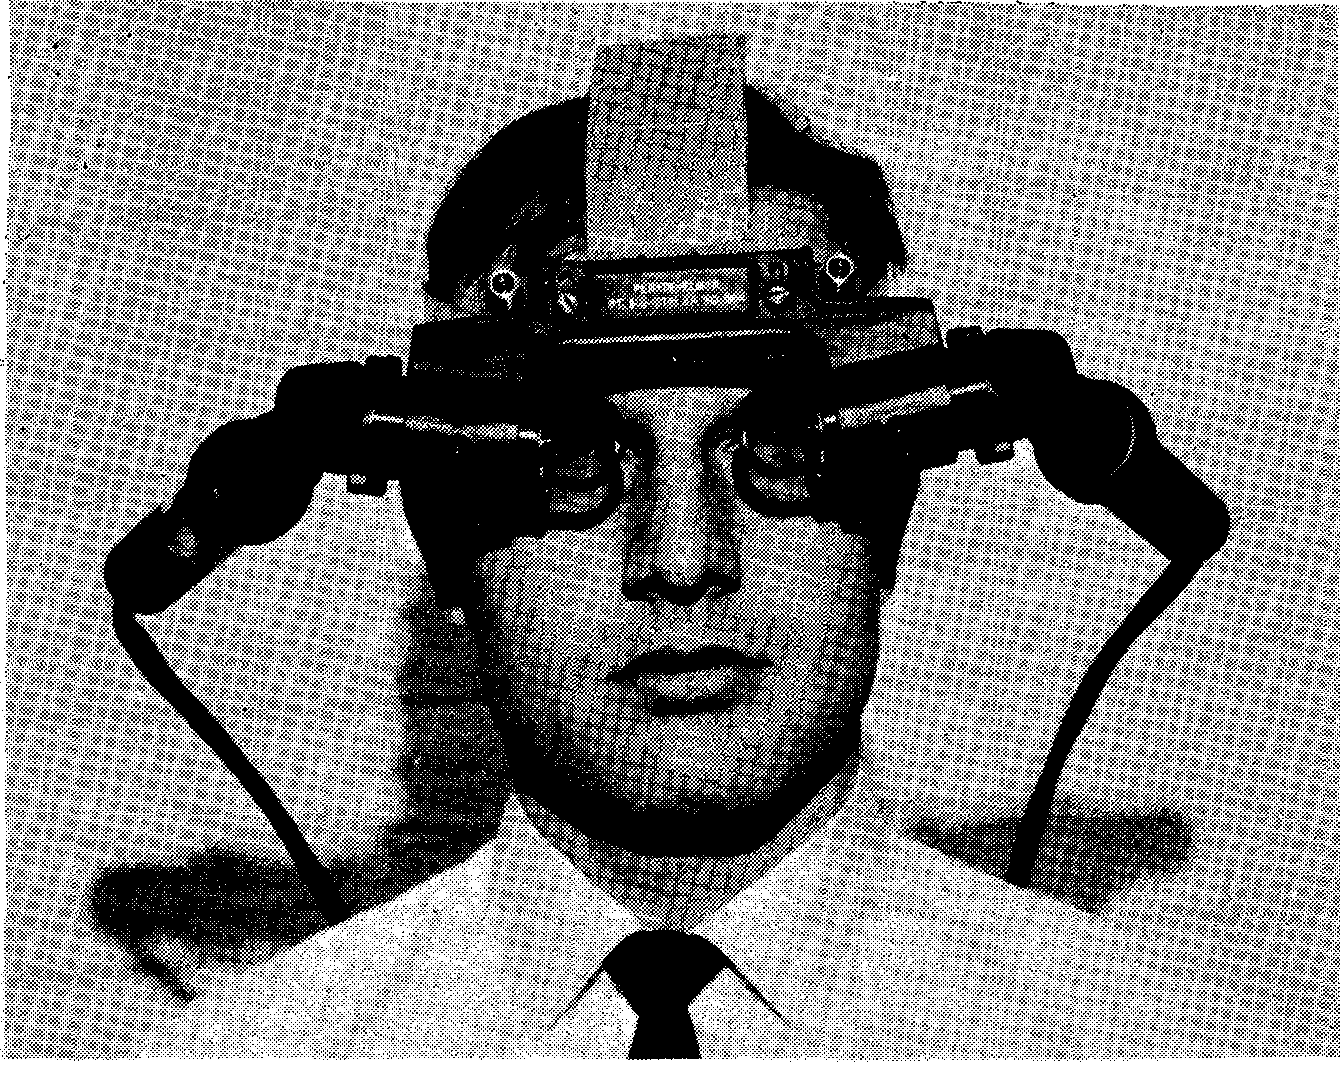
\includegraphics[keepaspectratio, width=0.6\textwidth]{Sutherland_HUD.png}
	\end{subfigure}
	\quad
	\begin{subfigure}[b]{0.45\textwidth}
		\centering
		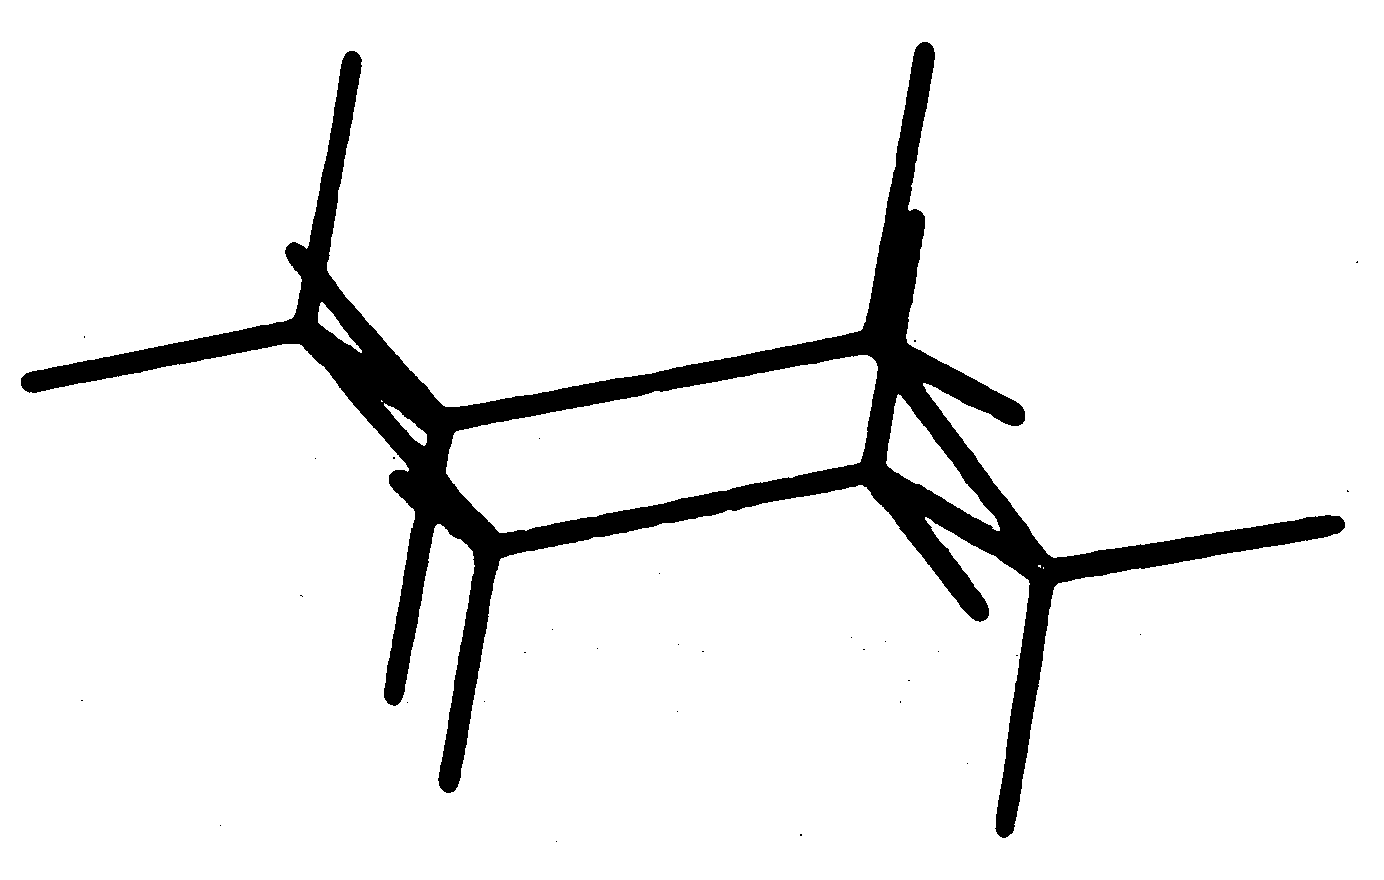
\includegraphics[keepaspectratio, width=0.6\textwidth]{cyclo-hexane_molecule.png}
		\caption{Modell eines Cyclohexanmoleküls, welches der Benutzer einblenden konnte}
	\end{subfigure}
	\caption{Sutherlands head-mounted display}
	\label{fig:FirstHUD}
\end{figure}

Der Term Augmented Reality selber wurde erstmals von \citeauthor{Milgram1994} im Jahre 1994 detailliert definiert, wobei sie die Vermischung der realen und virtuellen Welt betrachten und wohin die Technologie Augmented Reality fällt (siehe \ref{fig:RVContiinum}):

\vspace{1em}

\textquotedblleft the above-mentioned broad definition of Augmented Reality –  \textquoteleft augmenting natural feedback to the operator with simulated cues\textquoteright\ – is quite clear. Also noteworthy in this figure is the corresponding concept of Augmented Virtuality (AV), which results automatically, both conceptually and lexically, from the figure. \textquotedblright\ \parencite{Milgram1994}

\begin{figure}[htb]
	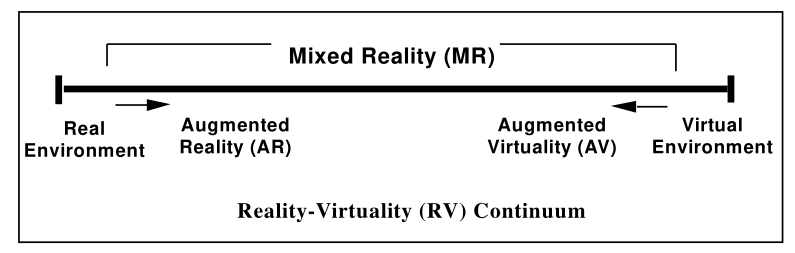
\includegraphics[keepaspectratio, width=\textwidth]{MR_milgram.png}
	\caption{Simplified representation of a RV continuum \parencite{Milgram1994}}
	\label{fig:RVContiinum}
\end{figure}

Fünf Jahre nach Milgram veröffentlichten \citeauthor{Kato1999} ihre Ergebnisse zu einem Marker-basierten AR Konferenzsystem. Sie lösten dabei das Problem der Registrierung (wo befindet sich der Benutzer, oder besser gesagt dessen Augen), und das Ermitteln der Pose (wie ist die Orientierung der virtuellen Kamera in Bezug zur Umwelt) über Marker mit einer fixen Grösse \parencite{Kato1999}. Das System wurde stationär mit Computern realisiert. In den folgenden Jahren wurden Versuche mit  mobilen Prototypen durchgeführt, diese blieben jedoch in der Grösse von Rucksäcken, und gebrauchten Notebooks mit der entsprechenden Rechenleistung (siehe Abbildung \ref{fig:MobileSysteme}).

\begin{figure}[h!]
	\centering
	\begin{subfigure}[t]{0.45\textwidth}
		\centering
		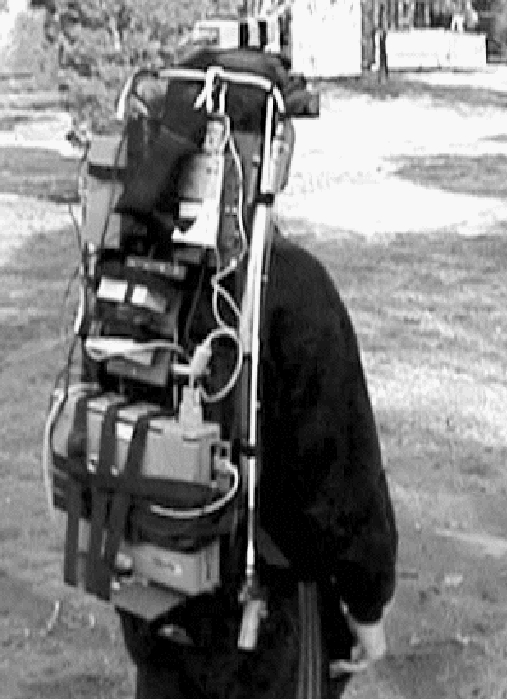
\includegraphics[keepaspectratio, width=0.4\textwidth]{tinmith2.png}
		\caption{Das TINMITH2 System \parencite{Thomas1999}}
	\end{subfigure}
	\quad
	\begin{subfigure}[t]{0.45\textwidth}
		\centering
		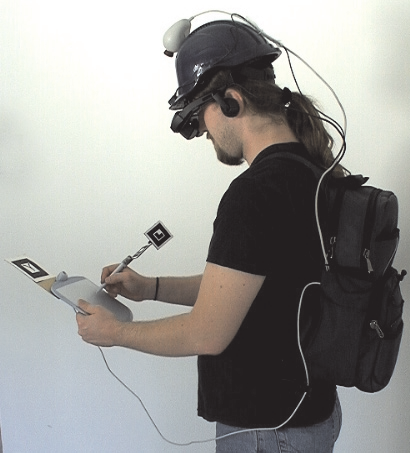
\includegraphics[keepaspectratio]{Studierstube2001.png}
		\caption{Interaktion mit der StudierStube Applikation \parencite{Reitmayr2001}}
	\end{subfigure}

	\begin{subfigure}[b]{0.45\textwidth}
		\centering
		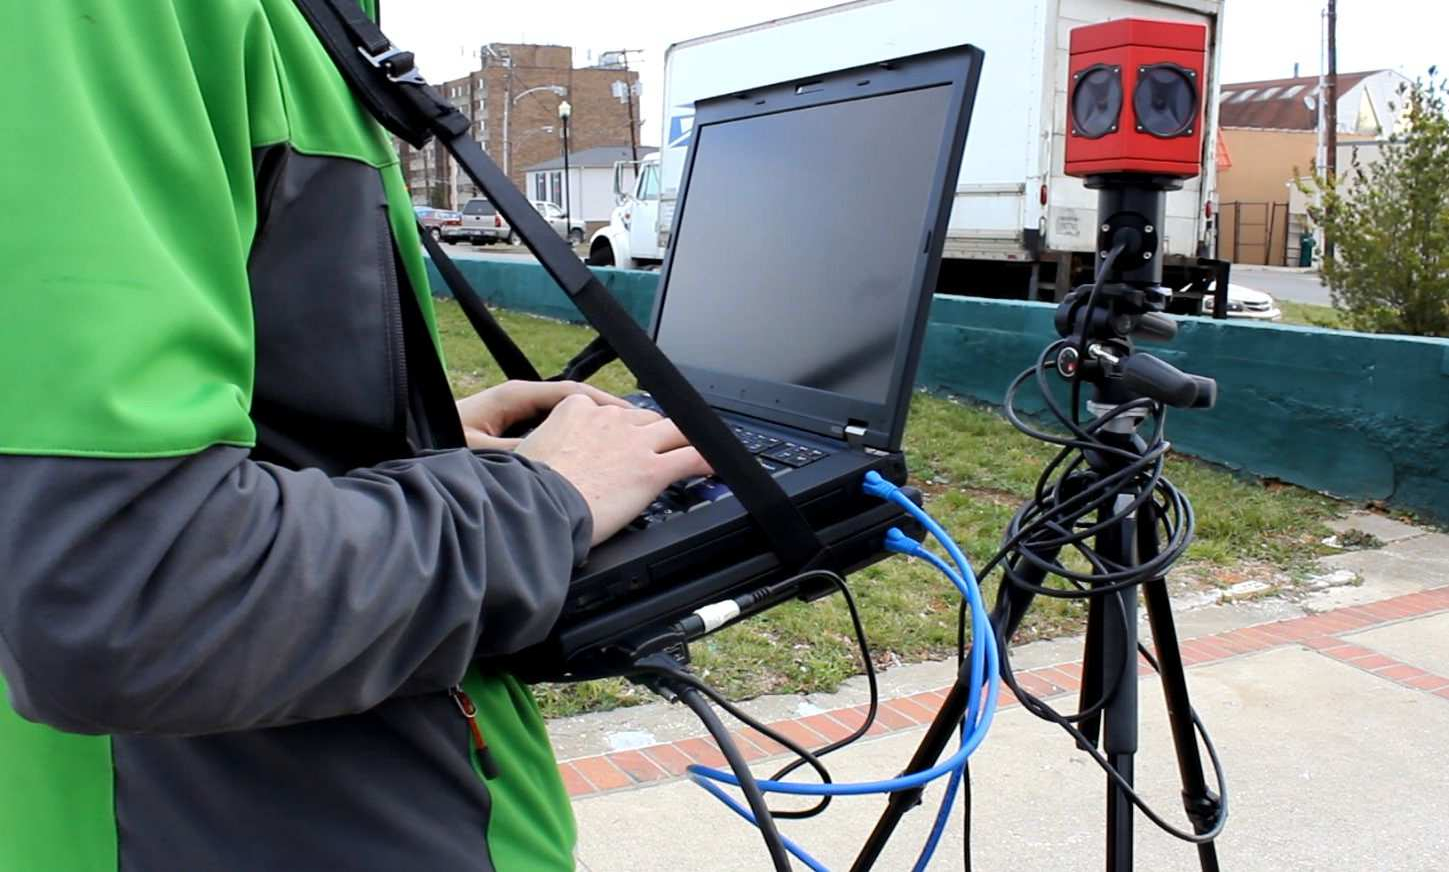
\includegraphics[keepaspectratio, width=0.6\textwidth]{LiveMobilePanoramicAR.png}
		\caption{\parencite{Cote2013}}
	\end{subfigure}
	\quad
	\begin{subfigure}[b]{0.45\textwidth}
		\centering
		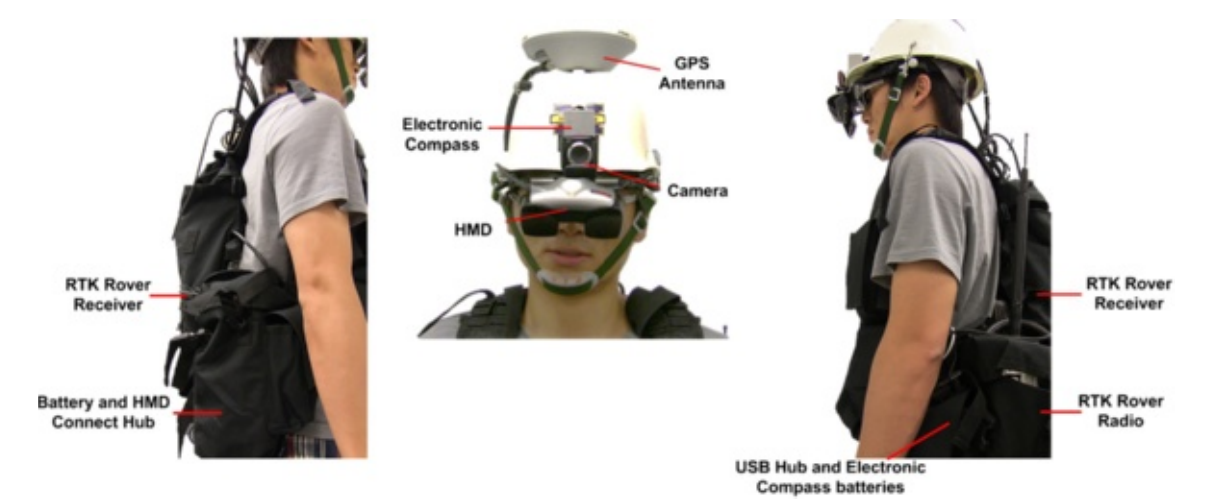
\includegraphics[keepaspectratio, width=0.8\textwidth]{ARMOR_System2013.png}
		\caption{Das ARMOR System \parencite{Dong2013}}
	\end{subfigure}
	\caption{Beispiele verschiedener mobiler Systeme}
	\label{fig:MobileSysteme}
\end{figure}

Ein grosser Durchbruch wurde deshalb von \citeauthor{Klein2009} erbracht, welche einen PTAM (Parallel Tracking and Mapping) Algorithmus auf einem iPhone 3G implementierten. Dieser war in der Lage sowohl in Räumen wie auch ausserhalb von Gebäuden, nach einer Initialisierungsphase die Lokalisierung von einem Marker loszulösen und die Pose der Kamera über \textquotedblleft Key Features\textquotedblright\ zu ermitteln \parencite{Klein2009}. Seither wurde auf diesem Gebiet weiter entwickelt und Algorithmen dieser Art sind unter dem Namen SLAM (Simultaneous Location and Mapping) zusammengefasst, dazu existieren verschiedene Frameworks welche diese nativ mitbringen (Kudan, wikitude).

\subsection{Konzepte}

\subsubsection{Markerbasierte Initialisierung}
Ein wichtiges Problem, das jede AR Applikation lösen muss, ist die Registration. Die Applikation muss also Koordinatensysteme und Ausrichtung der virtuellen Welt mit der realen Welt abgleichen und überwachen.

Optische Methoden (d.h. Analyse der Kameradaten) werden von gängigen Frameworks von Grund auf unterstützt. Zu diesen optischen Methoden gehören auch Marker. Ein Marker ist in den besten Fällen ein selbst unter Rotation und Scherung verformtes, eindeutig identifizierbares Muster, kann aber im Prinzip jegliches Bild sein. Ein guter Marker hat vorzugsweise einen hohen Kontrast im Grauspektrum, und grosse, komplexe Elemente ohne feine Details (welche auf Distanz verschwimmen oder verloren gehen) \parencite{Kudan2016}.

Die eigentliche Erkennung der Marker geschieht mit Algorithmen der Computer Vision (Kantenerkennung, Eckerkennung), worauf ein erkannter Marker mit einer Datenbank von bekannten abgeglichen wird. Danach kann über jenen einzelnen Marker sowohl Positionierung wie auch Lokalisierung geschehen.

\subsubsection{Markerless}
Da beim markerbasierten Tracking die namensgebenden \textquotedblleft Fiducial Markers\textquotedblright\ immer im Fokus der Kamera bleiben müssen, möchte man, falls möglich, diese gar nicht erst einsetzen müssen. Dies kann auf zwei verschiedene Arten erreicht werden: Modell-basiert und Feature-basiert \parencite{Ziegler2009}.

Ein modellbasiertes Tracking generiert aus einem physischen Objekt ein dreidimensionales, digitales Modell, welches verwendet wird die Pose zu kalkulieren. Üblicherweise werden diese Modelle aufgrund der Kanten oder Ecken des Objektes berechnet, Kanten sind dabei vorzuziehen, da Sie gegenüber wechselnden Lichtverhältnissen robust sind und durch den Computer effizient gefunden werden können \parencite{Zhou2008}. Dies bedeutet jedoch nicht, dass dies die beiden einzigen Möglichkeiten für ein Modellbasiertes Tracking sind. Sowohl \citeauthor{PauloLima2017} wie auch \citeauthor{Cote2013} gebrauchen in ihren Arbeiten Systeme, welche von Punktewolken ausgehend die jeweilige Pose ausrechnen.

Die Feature-basierte Methode extrahiert interessante Punkte eines Bildes und versucht diese auf subsequenten Bildern wiederzufinden. Wie diese Punkte identifiziert werden, hängt von der gewählten Methode ab. Bei SIFT (scale-invariant feature transform) sind dies beispielsweise die Minima/Maxima mehrerer Gaussschen Weichzeichnungsfunktionen \parencite{Lowe1999}. Bei nachfolgenden Bildern werden erneut Features bestimmt und mit den vorhergegangen abgeglichen. Erschwert wird der Prozess dadurch, dass zwei Bilder nicht unbedingt durch Transformationen (Rotation, Skalierung, Scherungen) ineinander überführt werden können. Es müssen also Features gefunden und erkannt werden, welche gegenüber solchen Transformationen resistent sind.

\subsubsection{SLAM}
Wie im vorherigen Paragraf erklärt, wird zwischen zwei markerless Tracking Methoden unterscheiden. Eine spezifische, die sogenannte SLAM Methode, wird in diesem Paragraf näher erklärt. Diese Methode identifiziert, mit Computer Vision, Feature-Points (ein Bildpunkt der sich durch seine lokale detaillierte Umgebung von anderen Punkten desselben Bilds hervorhebt), sowie deren Abhängigkeiten zueinander (Location) und fasst diese in einer Karte zusammen (Mapping). Sollte nun die Pose verloren gehen (durch einen Unterbruch des Kamerastream oder zu schnelle Bewegungen), muss nur ein Teil der vorherigen Karte wiedergefunden werden, um die Position wieder zu bestimmen. Dieser Ansatz wird \textquotedblleft Simultaneous Location and Mapping\textquotedblright (dt. Simultanes Erkennen und Kartografieren) genannt.

\subsection{GPS}
Das Global Positioning System (GPS) ist ein ursprünglich von dem amerikanischen Militär entwickeltes System von Satelliten. Jeder der Satelliten besitzt intern mehrere Atomuhren worüber er die so genannte \textquotedblleft composite clock\textquotedblright\ (CC) berechnet \parencite{GPSSysDesc2009}. Diese CC Zeit wird als Dienst des Standard Positioning Service (SPS) mit seiner Position zusammen als C/A (Coarse / Acquisition) transmittiert. Über mehrere solcher Signale von verschiedenen Satelliten kann schlussendlich die Position des Benutzers berechnet werden. Die C/A ergibt eine Genauigkeit von 13 Metern in 95\% der Fälle, ein genaueres Signal steht dem amerikanischen Militär über einen verschlüsselten Kanal dem Precise Positioning Service zur Verfügung.

Im Jahre 1983 wurde durch Präsident Reagan das GPS der Öffentlichkeit zur Nutzung freigegeben \parencite{Brustein2014}. Aus Angst vor Missbrauch jedoch mit einem verschlechterten Signal, was sich Selective Availability (S/A) nannte. Dieses SA wurde im Jahre 2000 durch Präsident Clinton abgeschafft und erlaubte von da an präzise Positionierung von bis zu 3 Metern in 95\% der Fälle für alle Nutzer. GPS Satelliten werden in drei Blöcke unterteilt wobei diese wiederum in Generationen differenziert werden \parencite{DoDGPS2008}. Mindestens 24 Satelliten sollen zu jeder Zeit operational sein, und im Moment sind 31 Satelliten operational, 1 Block 2A, 11 Block 2R, 7 Block 2R-M, und 12 Block 2F \parencite{NCOGPS2018}.

Neben dem amerikanischen GPS System existieren das chinesische BeiDou Navigation Satellite System (BDS) welches planmässig 2020 mit 35 Satelliten globale Abdeckung erreichen soll, das europäische Galileo System welches ebenfalls 2020 mit mehr als 24 Satelliten operational sein soll, das indische IRNSS welches aber nur den indischen Kontinent abdeckt, das japanische QZSS welches mit 7 Satelliten bis im Jahre 2023 den Ostasiatischen Raum abdecken soll, und das russische GLONASS System welches mit 24 operationellen Satelitten globale Abdeckung erreicht (\cite{NCOGPS2017}, \cite{IACPNTGLONASS2018}).

\section{Anwendungen}

Der Einsatz von virtueller oder gemischter Realität ist für die Fachbereiche Medizin und Konstruktion sehr interessant. Wie \citeauthor{Piroozfar2018} beschreiben, bringt ein gezielter Einsatz in der Konstruktionsindustrie verbesserte Kommunikation, besseres Verständnis eines Projektes, präzisere Planung, schnellere Entscheidungsfindung, und alles in allem eine erhöhte Sicherheit und Effizienz \parencite{Piroozfar2018}. \citeauthor{Pelargos2017} sehen den Mehrwert für die Medizin in Planung einer Operation und verbesserte, da nicht gleich kritisch, Ausbildung der beteiligten Fachkräfte \parencite{Pelargos2017}. Im Vergleich zu traditionellen pädagogischen Methoden bietet MR das Potential den Lernenden greifbarer zu motivieren, und gleichzeitig sowohl räumliches Vorstellungsvermögen, wie auch technische Fähigkeiten zu verbessern. Weiter erwarten sie eine erhöhte Retention des gelernten, da der Kontext des Lernstoffs direkter bei der Anwendung dessen ist.

Beide Gruppen identifizieren jedoch dasselbe Problem für die geringe Adoption von AR in deren relevanten Feldern: das Fehlen von performanter, komfortabler und auch bezahlbarer Hardware, die für diese Felder geeignet ist in Bezug auf Komfort und anderen Anforderungen (Hygiene, Sterilisierbarkeit usw.). Im Moment sind solche Geräte ein Nischenprodukt, was dazu führt, dass die Entwicklung eines solchen Produkts ein erhebliches Risiko darstellt (\cite{Piroozfar2018}, \cite{Pelargos2017}).

Im Bereich der Unterhaltungsindustrie hat AR hingegen schon längst Einzug gehalten. Zwei der grössten Spiele (Ingress und Pokémon Go!) wurden von Niantic Labs entwickelt und besitzen Nutzerzahlen in Millionenhöhe, beide finden in einer Spielwelt statt, die entweder auf unserer basiert (Pokémon Go!). Oder in einem Paralleluniversum (Ingress), in welchem Aktionen, die in der realen Welt durchgeführt wurde, Auswirkungen besitzt. Dennoch besteht bei beiden das gleiche Problem: Fälschung der Geolokation der spielenden Geräte durch die Benutzer und ein fehlendes Endziel (\cite{MRRX2015} und \cite{KamelBoulos2017}). Dies führte zu einer Stagnation und dem Verlust von Spielern, nachdem der initiale Ansturm vorüber war (\cite{Arif2017}, \cite{KamelBoulos2017}), dennoch trugen diese Spiele massgeblich dazu bei, ein öffentliches Verständnis von AR zu bilden. Es darf daher davon ausgegangen werden, dass dadurch die Hürde für die Entwicklung neuer Spiele tiefer geworden ist.

\subsection{Building Information Modelling}

Auch im Bereich des BIM (Building Information Modelling) wurden im Zuge der Fortschritte in AR verschieden Lösungen erarbeitet. Spezialisierte Fachlösungen wie beispielsweise die DAQRI Smart Glasses (welche für AR und BIM im Industrieumfeld eingesetzt werden) \parencite{DAQRI2018}, welche das Format Autodesk BIM 360 verwendet, um Sanitär-, Ventilation- und Elektroleitungen direkt im Gebäude darzustellen. Und somit Planungsprobleme zu identifizieren. Diese befindet sich im Moment jedoch noch im \textquotedblleft Early Adopter\textquotedblright-Status, und ist dementsprechend nicht ausgereift.

Das Team von Auto AR \parencite{Opperman2015} entwickelten ein System, welches es einem Benutzer erlaubt geplante Neubauten aus einem Auto zu begutachten. Dazu montierten sie auf einem Personenwagen eine omnidirektionale Panoramakamera, welche ihre Daten an einen Laptop im Wagen überträgt. Dieser bereitet das Bild auf, platziert das zu betrachtende Gebäude in der virtuellen Welt, und speist diese virtuelle Welt an ein Oculus Rift, welche vom Probanden getragen wird. Damit sieht dieser sowohl eine Projektion der realen Welt, wie auch das geplante Gebäude an dessen Stelle.

Eine andere Richtung wurde vom Frauenhofer Institut in Darmstadt \parencite{Olbrich2013} eingeschlagen. Sie entwickelten ein BIM Framework welches erlaubt, über bestehende Gebäudebestandteile Mehrinformationen anzuzeigen, und dies sowohl auf stationären Kioskcomputern, wie auch auf mobilen Geräten. Sie entwickelten dafür eine Server Client Infrastruktur, welche die Berechnungen der Pose und Szenendarstellung auf den Server auslagert, und so die schwächeren Endgeräte entlastet. Ihre eigens dafür entwickelte Infrastruktur erlaubt den Benutzer ebenfalls, Notizen über ein Objekt dynamisch auf diesem zu platzieren, sodass dies auf allen anderen Endgeräten ebenfalls erscheint.

\section{Benutzerführung in AR Applikationen}
In der heutigen Zeit ist die User Experience (dt. Erfahrung der Interaktion des Benutzers mit einem System) ein zentraler Bestandteil in der Entwicklung von Applikationen. Es gibt kaum noch erfolgreiche Anwendungen, welche nicht ein designiertes Team für die Entwicklung der User Experience besitzen.

Für die Entwicklung einer zweidimensionalen Applikation gibt es bereits heute genaue Vorgaben und Vorgehensmodelle, wie eine solche Applikation eine gute User Experience erreichen kann. Leider können nicht alle Vorgaben und Vorgehensmodelle auch für eine dreidimensionale Applikation verwendet werden. Da unsere Applikation eine Augmented Realitiy Applikation wird, trifft dies speziell zu.
Für die Entwicklung einer guten User Experience für eine AR Applikation gibt es jedoch unterschiedliche Ansätze und Empfehlungen, welche von verschiedenen Unternehmen veröffentlicht wurden.

\subsection{User Centered Design}
\begin{figure}[h!]
	\centering
	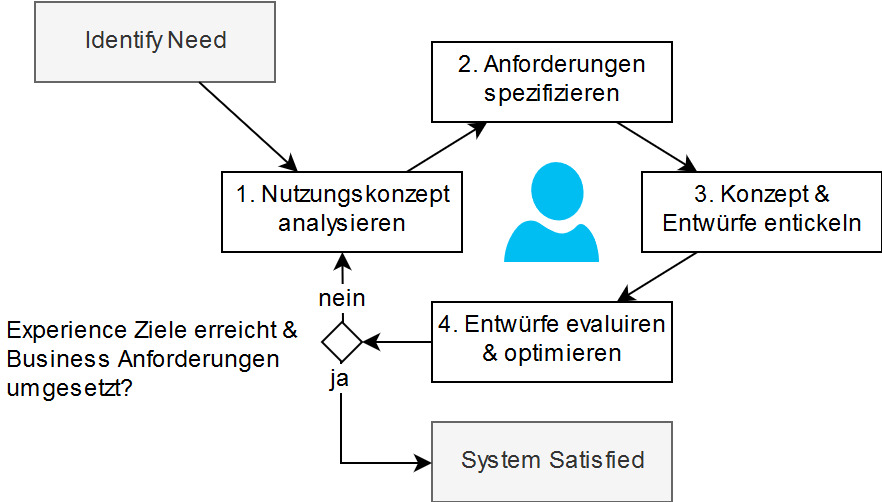
\includegraphics[keepaspectratio,width=0.8\textwidth]{UserCenteredDesign}
	\caption{Phasenmodell des ISO Standart 9241-210:2010 \parencite{ISO9241}}
\end{figure}

Um eine möglichst optimale User Experience zu erreichen, kann nach den Methoden des Standards ISO 9241-210:2010 (fortan als User Centered Design bezeichnet) vorgegangen werden. Dies ist ein iteratives Vorgehen, bei dem die Benutzer mit ihren Zielen, Bedürfnissen und Erwartungen über den gesamten Entwicklungsprozess hinweg im Zentrum stehen.
Jede Iteration dieses Prozesses durchläuft vier Phasen, bevor das Produkt in eine finale Version kommt.

Diese Methodik für die Ermittlung einer guten User Experience kann auch bei der Entwicklung einer AR Applikation verwendet werden.
In Phase 3 werden im User Centered Design zu Beginn meist Prototypen auf Papier entwickelt, mit welchem sich der Benutzter konzeptuell durch die Applikation navigieren muss. Diese Papierprototypen sind für eine dreidimensionale Applikation schwieriger zu gestalten und erschweren dadurch den Prozess. Bedingt durch diese Komplikation, ist der ganze Ablauf des User Centered Design teurer und komplexer (\cite{ISO9241}).

\subsection{Graphical User Interface Konzepte}
\label{ch:GraphicalUserInterface}
Im Rahmen des User Centered Designs gibt es zudem Richtlinien und Verhaltensweisen der graphischen Benutzeroberfläche.
Auch hier gilt, was bei zweidimensionalen GUI's funktioniert, kann oder muss nicht zwingend bei einer AR Applikation verwendet werden. Um die Interaktion mit der AR Applikation möglichst einfach und intuitiv zu gestalten, müssen folgende Punkte mit Sicherheit beachtet werden.

\subsubsection{Bildschirmflächenoptimierung}
Eine AR Applikation vermittelt den Eindruck, dass die physikalische Welt die Limitierung der Applikation ist, in Wahrheit ist jedoch der Bildschirm des Anzeigegerätes die eigentliche Limitierung.
Der Benutzer möchte also möglichst wenig von seiner eigentlichen Intention, zum Beispiel der Besichtigung eines Gebäudes von aussen, abgelenkt werden. Dies setzt voraus, dass die Informationen sowie Interaktionsmöglichkeiten weitgehendst konsolidiert werden.

\subsubsection{Vereinfachter Einstieg}
Selbst in einer zweidimensionalen Applikation ist die Einarbeitung in eine Applikation teilweise sehr schwierig und zeitaufwendig. In einer dreidimensionalen Applikation gestaltet sich dies jedoch noch um einiges schwieriger und ist meist mit einer grösseren Lernkurve verbunden, weshalb der Einstieg ein noch wichtigerer Aspekt bei der Entwicklung sein muss.

\subsubsection{Vorhersehbarkeit}
Ein Benutzer bringt durch seine Bildung wie auch seine Herkunft Erwartungen mit. Dieses antrainierte Verhalten sollte eine Applikation wo immer möglich nutzen und sinnvoll wiederverwenden. Als antrainiertes Verhalten gelten zum Beispiel Gesten zur Vergrösserung und Rotation einer Anzeige. Wo immer möglich sind solche intuitiven Aktionen einer Interaktion durch Buttons und Menüs vorzuziehen.

\subsubsection{Hinweise}
Der Mensch sucht stets nach Hinweisen und Signalen. Dieses Verhalten widerspiegelt sich auch in alltäglichen Situationen wie beispielsweise einer Bahnfahrt, auf welcher wir stets nach Symbolen und Hinweise für die nächste Haltestelle oder Ausfahrt Ausschau halten.
Solche Hinweise sollen in einer AR Applikation den Benutzer ermutigen die Applikation noch weiter zu erkunden.
Diese Hinweise müssen nicht zwingend Texte sein, so kann auch ein Pfeil in die Richtung deuten, in welche sich das anzuzeigende Objekt befindet, sobald dieses aus dem Bildschirm tritt.

\subsubsection{Vielfältige Benutzer}
Eine AR Applikation soll stets für eine Vielzahl von Benutzer brauchbar sein. Dies soll besonders berücksichtigt werden, wobei auf Beeinträchtigungen wie Farbenblindheit oder ähnliche Konditionen geachtet werden sollte (\cite{AppleGuideline2018}, \cite{GoogleGuideline2018}, \cite{GoogleIO2018}, \cite{BerfinAyhan2017}).

\chapter{Lösung}
Im folgenden Kapitel wird die Lösung beschrieben. Es soll ein Überblick über die Umsetzung der Applikation geboten werden. Eine detaillierte Beschreibung ist in Kapitel \ref{sec:SysSpec} zu finden. Es wird zudem ein alternatives Konzept vorgestellt, welches nicht weiter verfolgt wurde.

\section{Konzeptionelle Idee}
\label{ch:KonzeptionelleIdee}
Wie in Kapitel \ref{ch:StandDerForschung} beschrieben, kann eine AR Applikation markerless oder markerbasiert sein. Dabei gibt es auch bei diesen zwei Kategorien unterschiedliche Möglichkeiten diese zu realisieren. Obwohl beim markerbasierten Tracking für die Initiierung und Platzierung ein Marker verwendet werden muss, so ist dies beim markerless Tracking nicht nötig. Da markerless Tracking jedoch ein Objekt nicht ohne weitere Anhaltspunkte auf dem Bildschirm darstellen kann, muss bei markerless Tracking eine Alternative zum Marker gefunden werden. Dies kann beispielsweise die Erkennung von Flächen sein \parencite{GoogleARCore2018} oder auch Lokalisierungssensoren.
Um eine AR Applikation zu entwickeln, welches ein Gebäude in der realen Umgebung darstellt, würden sich potenziell beide Lösungen, also auf Marker basierend wie auch markerless Tracking, anbieten.
Im Rahmen des Projektes wurde zuerst eine markerless wie auch eine markerbasierte Lösung parallel entwickelt. Jedoch stiessen wir beim markerbasierenden Konzept auf Probleme, auf welche in Kapitel \ref{ch:verworfeneLösungen} näher eingegangen wird, wodurch Lösung nicht weiter verfolgt wurde.


\bigbreak
Das Konzept einer auf Lokalisierungssensoren basierten Lösung sieht vor, dass das darstellende Gerät über folgende zusätzliche Komponenten verfügt:
\begin{enumerate}
	\item Lokalisierungssensor (GPS/GLONASS/BEIDOU/GALILEO Sensor)
	\item Kompass
	\item Gyroskop
\end{enumerate}

Bei dieser Lösung werden die Lokalisierungssensoren sowie der Kompass dazu verwendet die Positionierung des darzustellenden Gebäudes zu berechnen. Die lokalen Bewegungen des Anzeigegerätes würden mithilfe des Gyroskops ausgelesen, und dazu verwendet das Gebäude an Ort und Stelle zu halten.
Nachteil dieser Methode liegt darin, dass die Anzeige nun abhängig von drei Sensorwerten ist, welche selber jeweils eine Ungenauigkeit aufweisen und damit Fehler ins System einbringen. Dieser Umstand kann dazu führen, dass das anzuzeigende Gebäude nicht immer an der exakten Position dargestellt wird.
Der Vorteil liegt darin, dass neue Objekte welche dargestellt werden sollen, sehr einfach hinzugefügt werden können.

\section{Applikationsablauf}
Die Applikation durchläuft verschiedene Schritte, damit sie dem Benutzer das Modell in der Umgebung an der korrekten Position anzeigen kann. Diese Schritte sind anhand der Abbildung  \ref{fig:Ablaufdiagramm} grafisch dargestellt.

\begin{figure}[h!]
	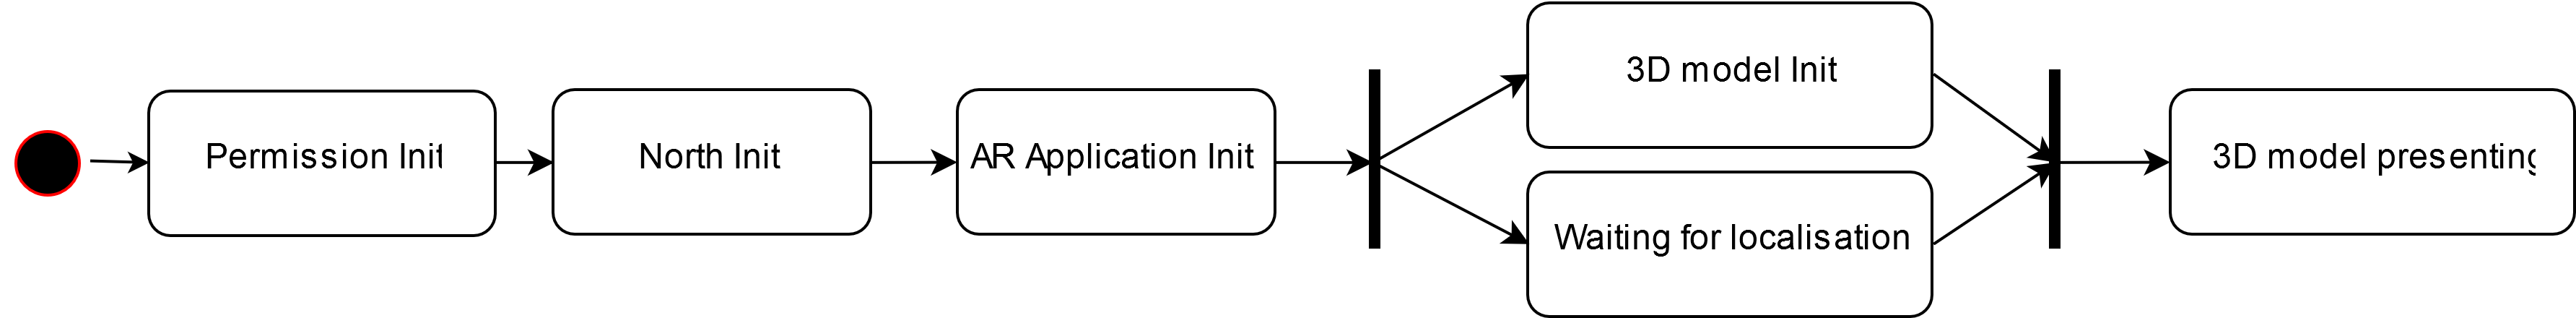
\includegraphics[keepaspectratio, width=\textwidth]{AblaufdiagrammARApplikation.png}
	\caption{Ablaufdiagramm der AR Applikation}
    \label{fig:Ablaufdiagramm}
\end{figure}

\subsection{Permission Init}
Sobald die Applikation startet, werden diverse Berechtigungen überprüft, welche die Applikation für den normalen Gebrauch benötigt. Dazu gehören folgende Berechtigungen:
\begin{itemize}
\item Zugriff auf Kamera
\item Zugriff auf Lokalisierungssensoren
\item Speicherzugriff (um Modelle laden/speichern zu können)
\end{itemize}
Sind gewisse Berechtigungen nicht vorhanden, so werden diese in diesem Status beim Benutzer nachgefragt. Hierfür werden dem Benutzer alle fehlenden Berechtigungen in einer Liste dargestellt. Damit der Benutzer nicht in einer Endlosschlaufe die Berechtigungen ablehnt, wird nur einmal nach den Berechtigungen gefragt und anschliessend lediglich auf Wunsch des Benutzers erneut gefragt. Es ist zwingend notwendig, dass der Benutzer diese Berechtigungen zulässt, da die ganze Applikation ansonsten nicht funktionsfähig ist. Hat der Benutzer allen Berechtigungen zugestimmt oder hat die Applikation schon alle Berechtigungen, wechselt der Status auf den im Kapitel \ref{ch:NorthInit} beschriebenen Zustand. Die Abbildung \ref{fig:PermissionInitStatus} stellt die Grafische Benutzeroberfläche der Abfrage dar.
\begin{figure}[h!]
	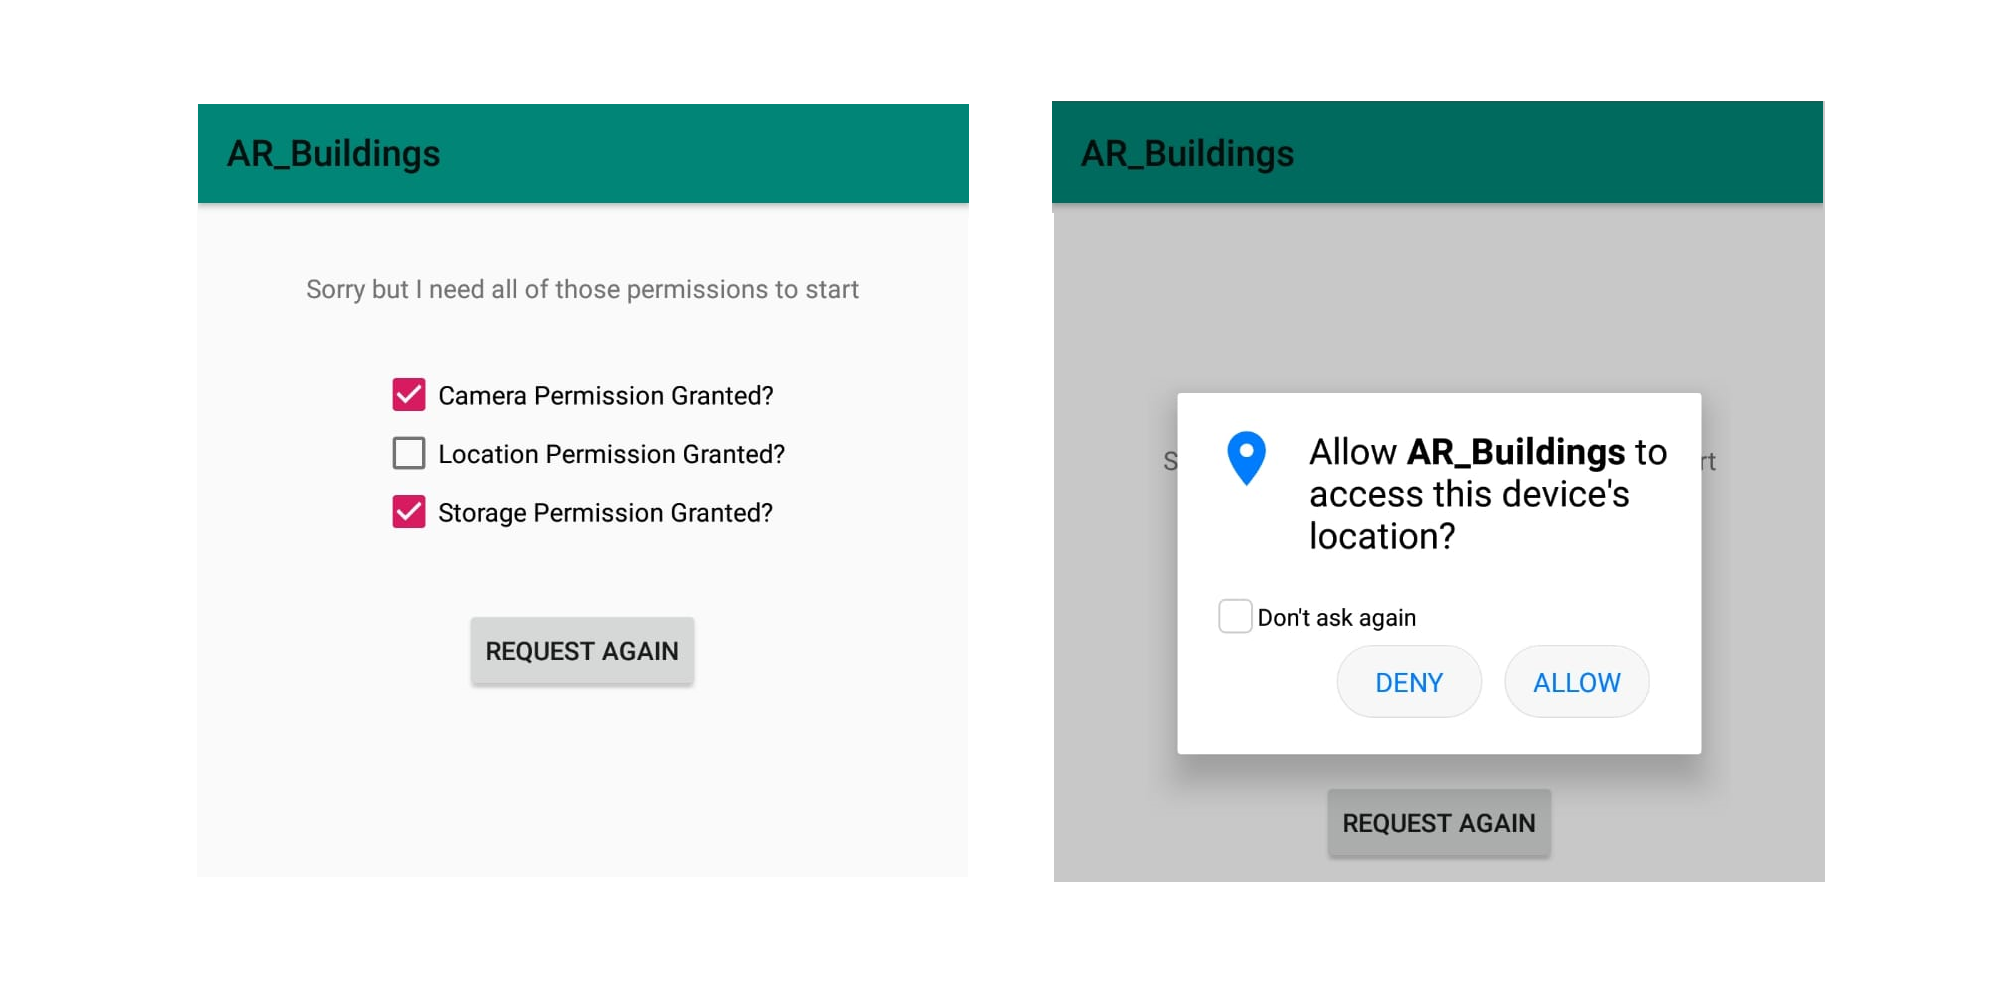
\includegraphics[keepaspectratio, width=\textwidth]{ARBuildingPermissionRequest.png}
	\caption{Darstellung und Abfrage fehlender Berechtigung}
    \label{fig:PermissionInitStatus}
\end{figure}

\subsection{North Init} \label{ch:NorthInit}
In diesem Status wird versucht den Norden mittels Kompass auszulesen und dem Benutzer visuell dessen Richtung angezeigt. Dabei wird der Benutzer dazu aufgefordert das Smartphone nach Norden auszurichten. Dies dient dazu, dass das virtuelle Koordinatensystem welches Kudan in sich aufbaut, mit dem Physischen Koordinatensystem übereinstimmt.

Sobald der Benutzer das Gerät genug lange nach Norden ausgerichtet hat, startet die Applikation in den in Kapitel \ref{ch:ARApplicationInit} beschriebenen Status. In der Abbildung \ref{fig:NorthInitProcess} ist die Grafische Benutzeroberfläche für die Initialisierung dieses Schrittes zu sehen.
\begin{figure}[h!]
	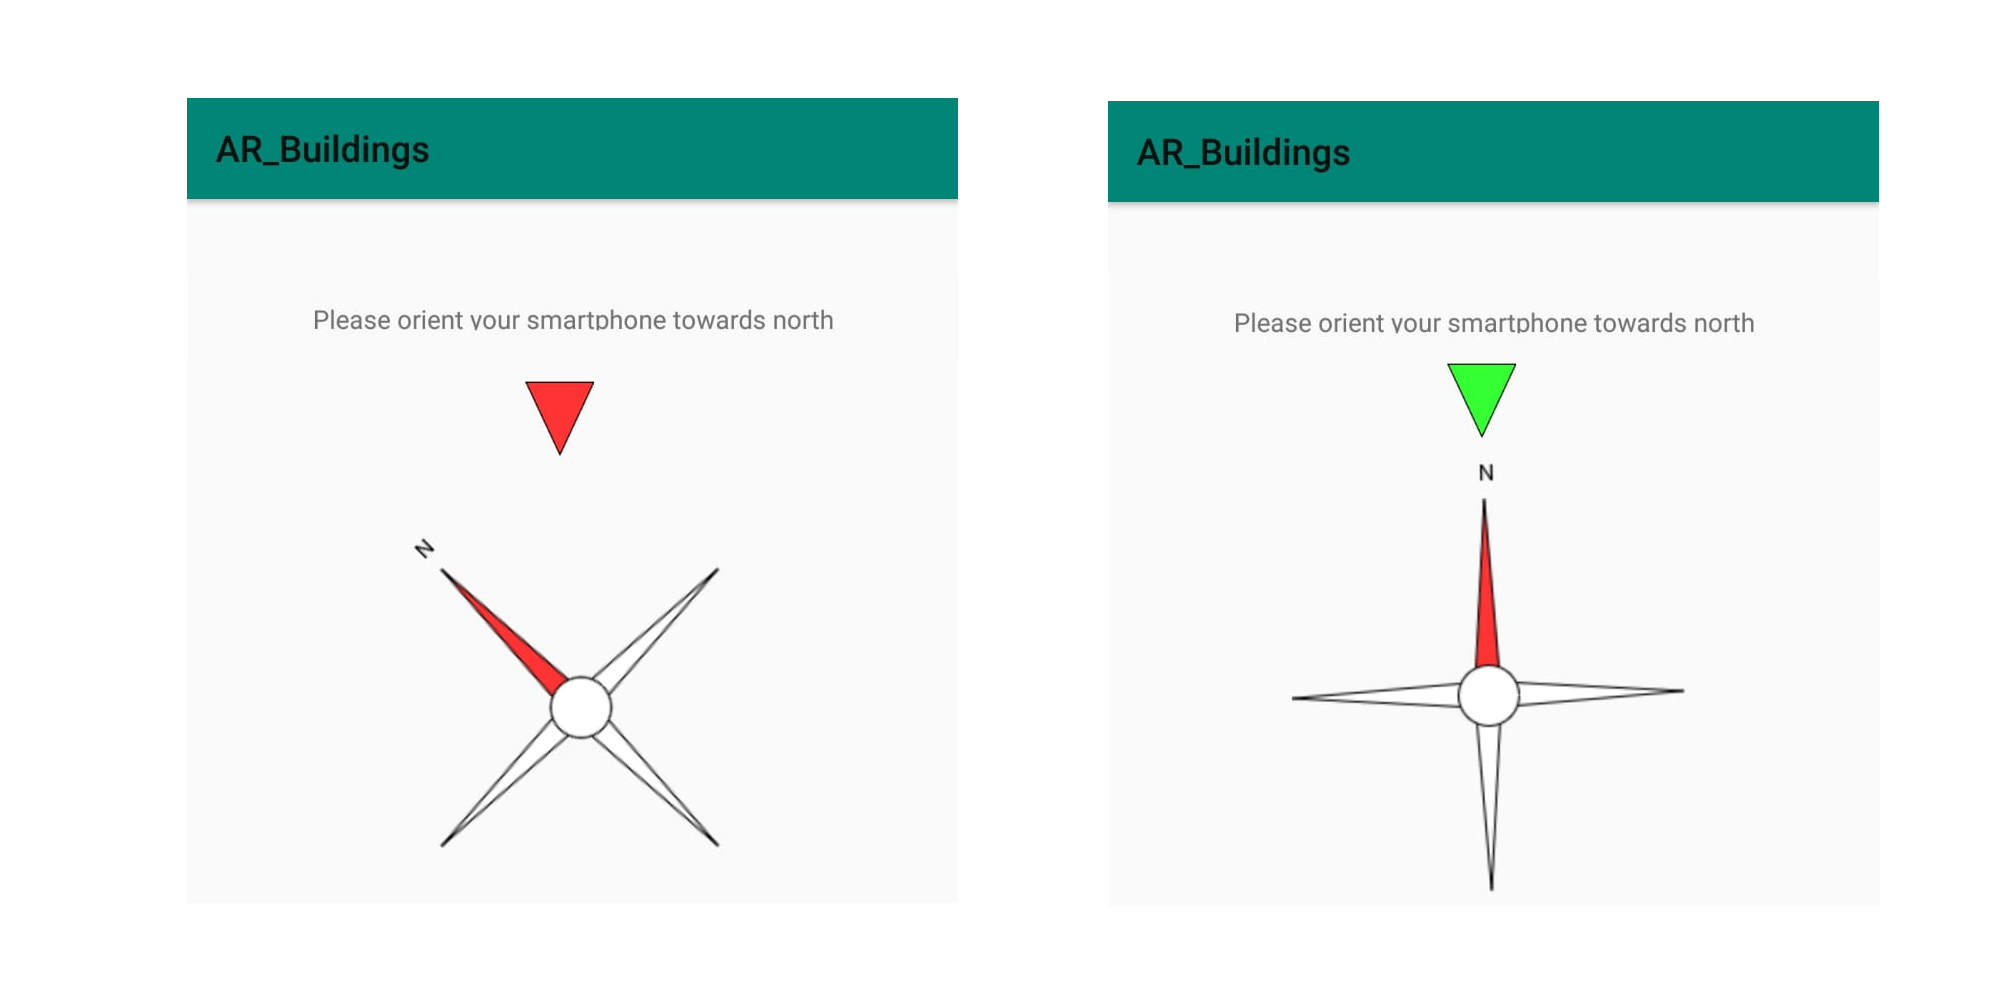
\includegraphics[keepaspectratio, width=\textwidth]{NorthInitProcess.png}
	\caption{Darstellung North Init mit Indikator ob richtige Position erreicht wurde.}
    \label{fig:NorthInitProcess}
\end{figure}

\subsection{AR Application Init} \label{ch:ARApplicationInit}
Kommt die Applikation in diesen Status, werden alle notwendigen Schritte für die Initialisierung der AR Applikation gestartet. Dies bedeutet insbesondere, dass die Kudan AR Welt aufgebaut wird. Zudem abonniert dieser Status den Event, welcher bei Aktualisierungen der Lokalisierung des Gerätes geworfen wird und wechselt zum Status, welcher in Kapitel \ref{ch:waitingForLocation} beschrieben ist.

\subsection{3D Model Init}
Dieser Status \textquotedblleft 3D Model Init\textquoteright\ erfüllt zum jetzigen Zeitpunkt noch keinen Zweck. Er würde jedoch die Modelle, welche die Applikation darstellen soll von einer Website herunterladen und diese der Applikation bereitstellen.

\subsection{Waiting for localisation} \label{ch:waitingForLocation}
In diesem Schritt wird gewartet, bis eine valide Position vom Gerät zurückgegeben wird. Die Position wird als valide betrachtet, sobald sie eine Genauigkeit von unter 10m aufweist. Der Benutzer wird auch hier über den Zustand der Applikation informiert (siehe Abbildung \ref{fig:KoordinationNotFound}), indem eine Grafische Darstellung dem Benutzer mitteilt, dass zurzeit keine Daten über die Position vorhanden sind um das Gebäude darzustellen. Der Status wechselt automatisch in den in Kapitel \ref{ch:ThreeDModelPresenting} beschriebenen Zustand, sobald sich dies ändert.

\begin{figure}[h!]
	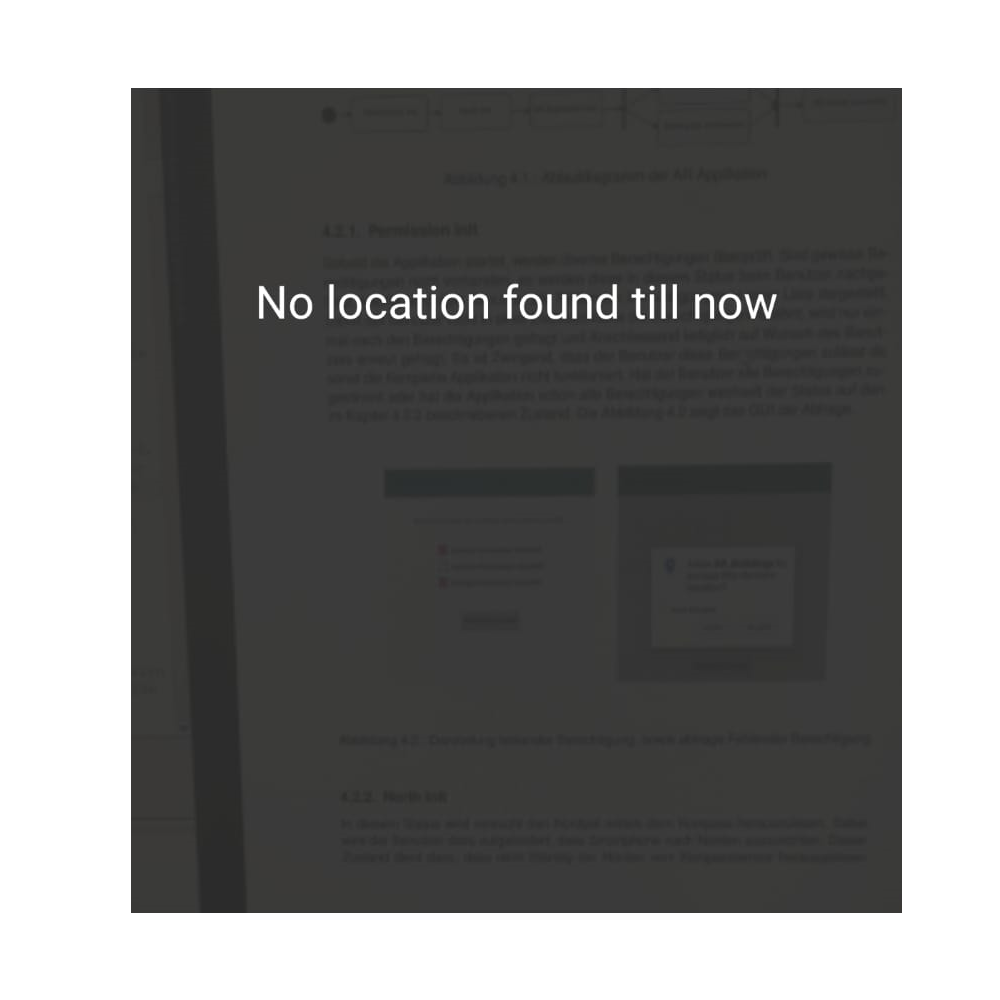
\includegraphics[keepaspectratio, width=\textwidth]{UnknownLocation.png}
	\caption{Darstellung solange Position unbekannt ist.}
    \label{fig:KoordinationNotFound}
\end{figure}


\subsection{3D Model presenting} \label{ch:ThreeDModelPresenting}
In diesem Schritt wird das Model für den Benutzer dargestellt. Das Modell wird mittels des Kudan Frameworks auf derselben virtuellen Position gehalten. Dazu wird der Gyroskopsensor ausgewertet um die Ausrichtung des Smartphones zu ermitteln. Bewegt sich der Benutzer in der Physikalischen Welt und neue Lokalisationsdaten treffen ein, werden diese verwendet um die Lokalisation des dargestellten Objektes neu zu berechnen und Anzuzeigen. 
Der Benutzer kann von diesem Zustand wieder in folgenden Zustand kommen:

\begin{itemize}
	\item North init (Durch Klicken auf entsprechenden Button siehe Abbildung \ref{fig:ARShowBuilding})
\end{itemize}

\begin{figure}[h!]
	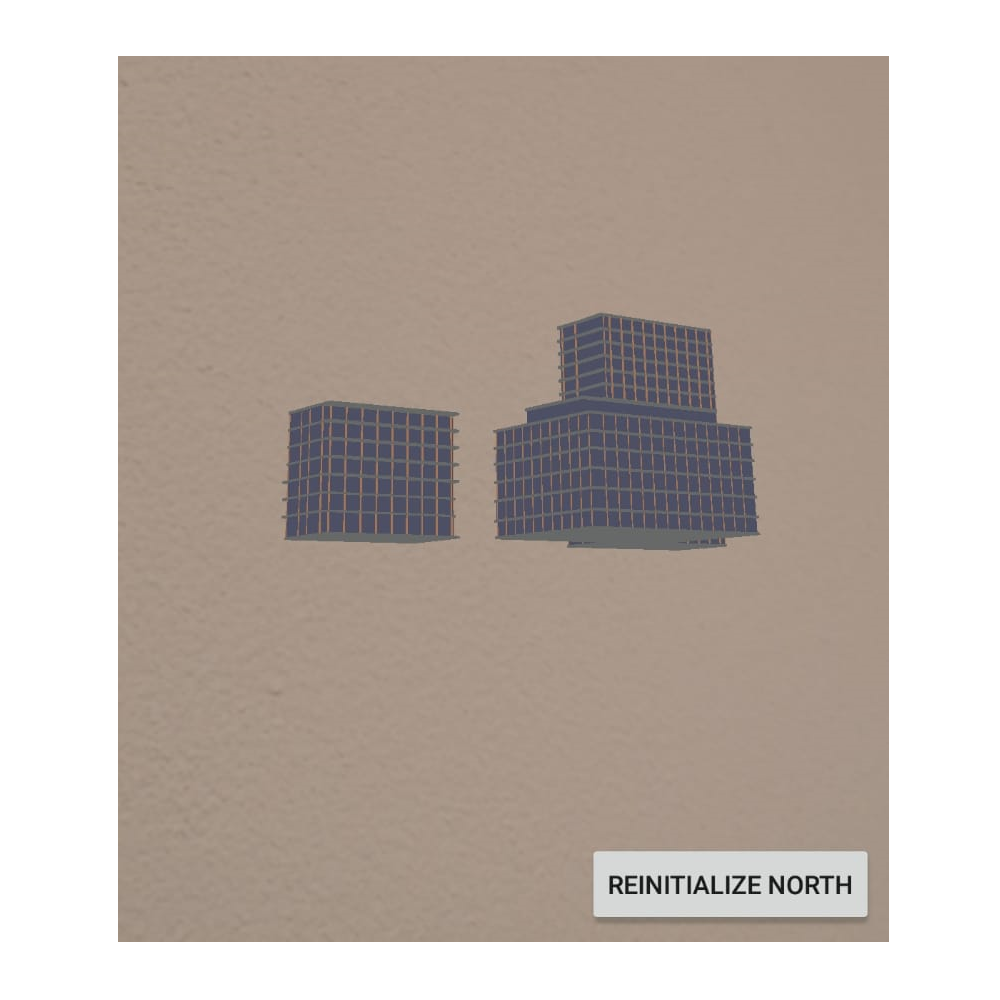
\includegraphics[keepaspectratio, width=\textwidth]{ARShowBuilding.png}
	\caption{Darstellung des Gebäudes sobald die Position ausfindig gemacht werden konnte (hier gefälschte Positionsdaten).}
    \label{fig:ARShowBuilding}
\end{figure}

\clearpage

\section{Verworfene Lösungen}
\label{ch:verworfeneLösungen}
Insgesamt wurden vier Prototypen entwickelt, von denen drei verworfen wurden. Es wurde dabei jeweils zwei Mal das gleiche Konzept auf verschiedener Entwicklungsumgebungen aufgebaut. So wurde zuerst die konzeptionelle Idee aus Kapitel \ref{ch:KonzeptionelleIdee} mit Unity entwickelt. Zudem wurde ein zweites Lösungskonzept (siehe Kapitel \ref{ch:markerbasiertesLoesungskonzept} simultan zum gewählten Konzept entwickelt, welches jedoch nach der Prototypenphase verworfen wurde. Auch dieser Prototyp wurde zuerst mit Unity und anschliessend mit AndroidStudio entwickelt (Gründe dafür sind in Kapitel \ref{ch:evaluation} zu finden).

\subsection{Markerbasiertes Lösungskonzept}
\label{ch:markerbasiertesLoesungskonzept}
Das Konzept eines markerbasierten Lösung sieht vor, dass die Position des Markers in der realen Welt bereits bekannt ist, und sich diese nicht ändert. Sofern dies der Fall ist, kann die relative Position der Kamera zum Marker und somit zum Gebäude berechnet werden.

Die relative Position zum Marker kann durch dessen Grösse sowie dem Winkel in Relation zur Ausrichtung der Kamera berechnet werden. Sobald diese relative Position berechnet werden konnte, kann die relative Position zum Gebäude ausgerechnet werden.

Der Vorteil dieser markerbasierten Lösung liegt darin, dass die Genauigkeit der Darstellung unabhängig von weiteren Faktoren ist. Die grosse Schwäche liegt darin, dass ein Marker an einer fixen Stelle befestigt werden muss. Zudem ist es aufwendiger neue Gebäude hinzuzufügen, da man den Marker physisch vor Ort platzieren muss.

\subsection{Prototyp}
Um dieses Konzept zu realisieren, wurde ein Prototyp entwickelt. Bei diesem wurde jedoch ein schwerwiegendes Problem identifiziert. Nämlich, dass das Gebäude aus nicht weiter untersuchten Gründen beim gleichen Marker immer wieder verschieden dargestellt wurde. Dieses Verhalten führte dazu, dass die Parallele Entwicklung dieses Konzeptes eingestellt wurde, und der Fokus auf die auf der Position basierte Lösung gelegt wurde. In Abbildung \ref{fig:alternativeSolution} sieht man das Fehlverhalten des 3D Modells.

\begin{figure}[h!]
	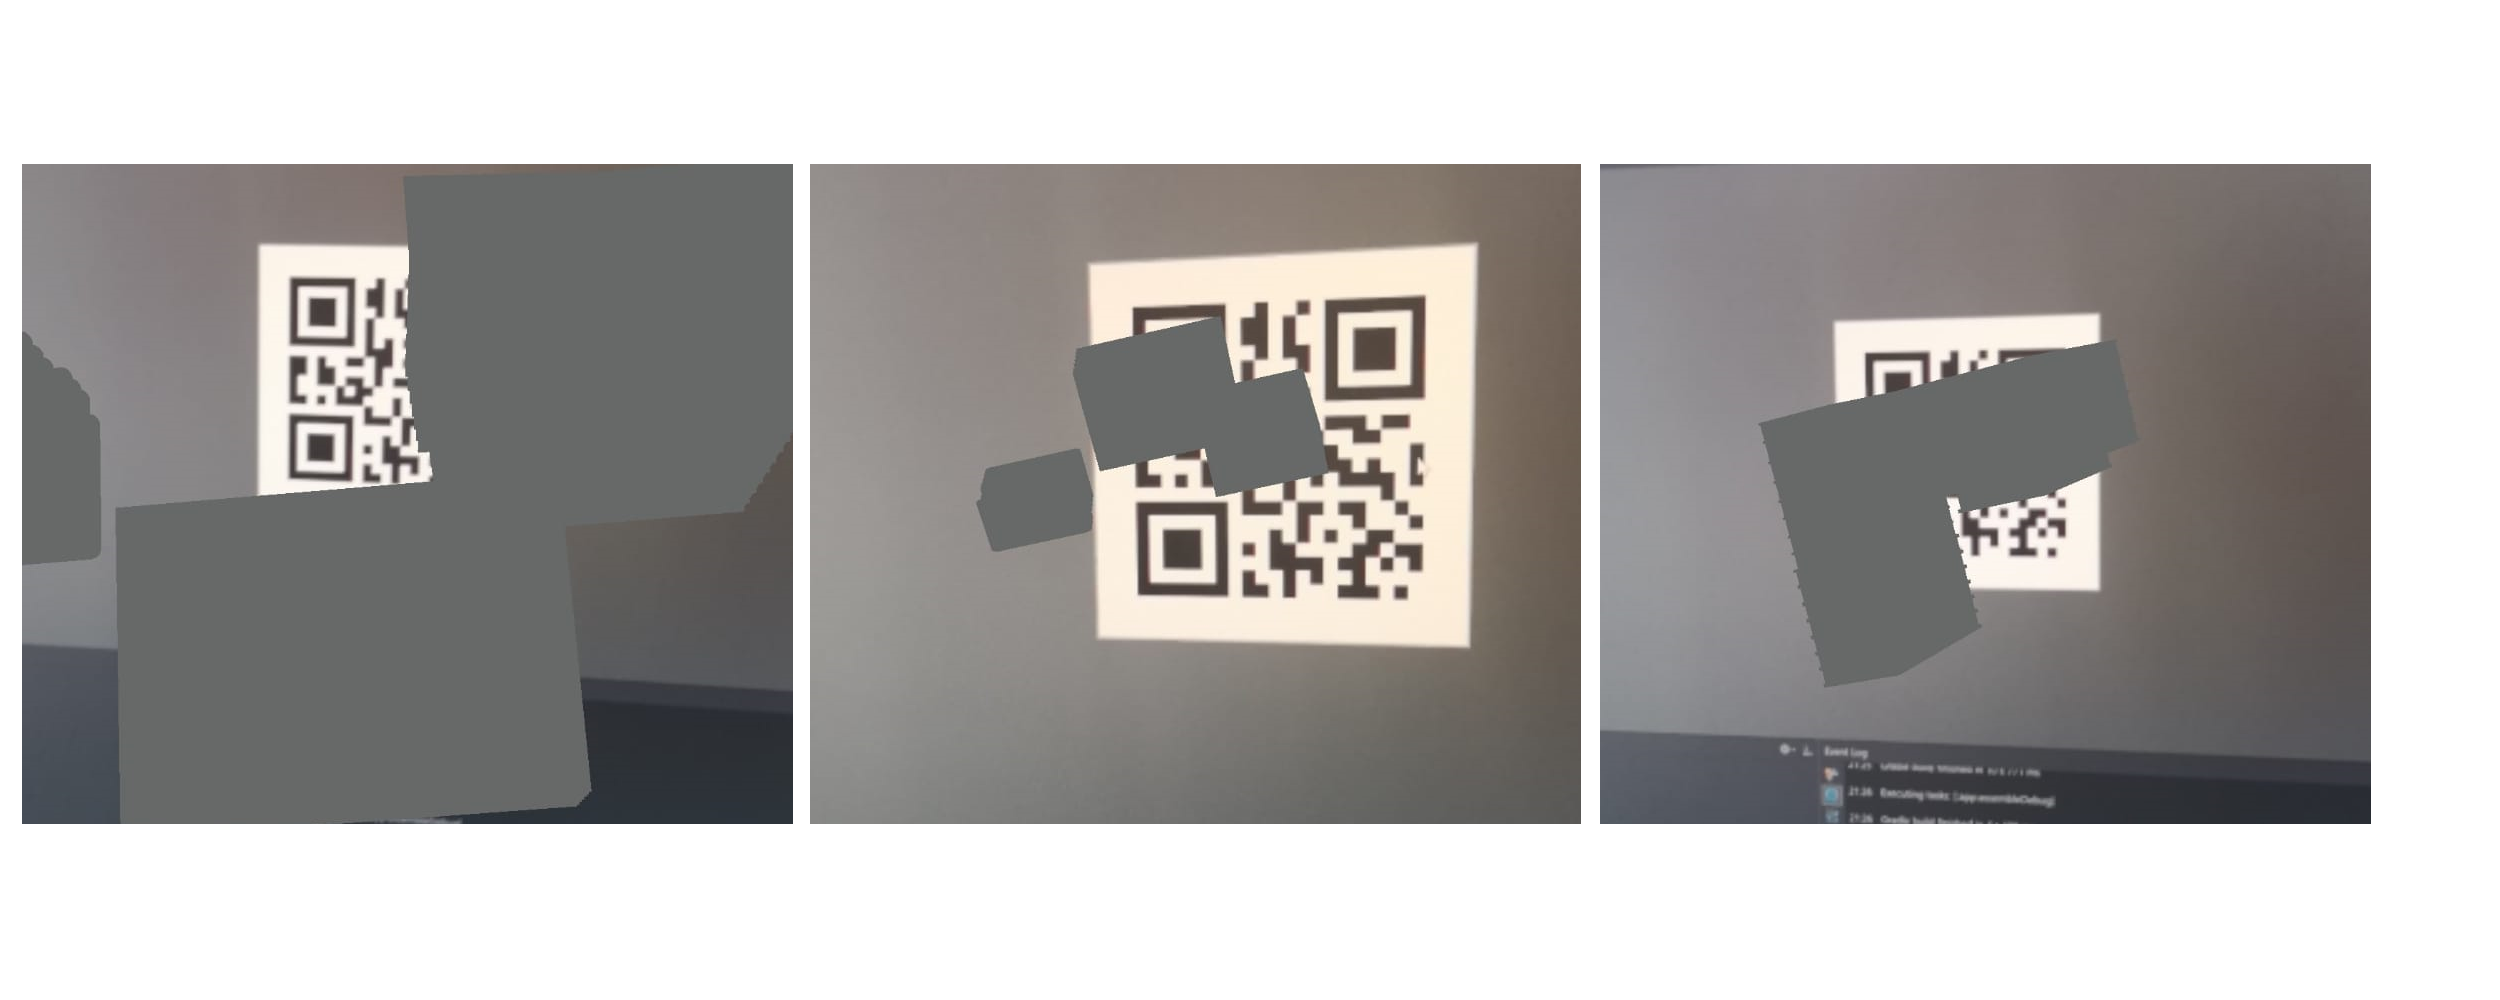
\includegraphics[keepaspectratio, width=\textwidth]{alternativeLoesung.png}
	\caption{Verworfene Alternative Lösung, Problem der unterschiedlichen Darstellungen des Gebäudes.}
    \label{fig:alternativeSolution}
\end{figure}

\chapter{Technische Beschreibung}

\section{Projektinformationen}

\subsection{Vorgehensmodell}

Alle Wirtschaftsprojekte an der Hochschule Luzern fallen in eine der folgenden Kategorien:

\begin{enumerate}
	\item Einsatz von Standardsoftware und Services
	\item Software- und Produktentwicklung
	\item Innovationsprojekt
	\item IT-Infrastrukturentwicklung
	\item Strukturierte Analyse und Konzeption von Systemen und Abläufen
\end{enumerate}

Dabei ist dieses Projekt als Innovationsprojekt und Softwareentwicklung klassifiziert worden. Wir erwarteten daher unter anderem, eine Evaluation, Recherchen und weitere Unbekannten. Um auf diese eingehen zu können, entschied sich das Team dafür die hybride, inkrementelle Agile Methode zu verwenden.

\subsection{Agile Projektmethode}

Die agile Projektmethode zielt darauf ab in einem ungewissen und sich verändernden Umfeld zu bestehen. Insbesondere bedeutet dies, das auf sich verändernde Voraussetzungen schnell reagiert werden kann und dabei ein funktionierendes Produkt entsteht \parencite{AgileAlliance2015}. Dies soll durch eine enge Zusammenarbeit mit dem Auftraggeber und guter teaminterner Kommunikation erreicht werden.
\bigbreak
Ein Rahmenplan dient als Richtschnur des Projektes, während die Anforderungen in den jeweiligen Sprints spezifiziert werden, und in der Sprintplanung festgehalten wird. Wir unterteilten unser Projekt in eine zweiwöchige Initialisierung, zweiwöchige Evaluation, und fünf Sprints, in der unser Produkt entwickelt wurde.

\subsection{Ermittlung offener Projektrahmenbedingungen}
\label{ch:evaluation}
Im Rahmen dieses Projektes mussten verschiedene Unbekannte zuerst analysiert und evaluiert werden. Dazu gehörten die Zielplattform, Entwicklungsumgebung und die zu verwendenden Augmented Reality Frameworks.
\subsubsection{Zielplattform}
Als Zielplattform standen gemäss Projektbeschrieb die Folgenden zur Auswahl:
\begin{itemize}
\item Microsoft HoloLens
\item Smartphone und Tablets
\end{itemize}
Für alle dieser Plattformen galt die Idee, sie als Interface zu gebrauchen um das AR Gebäude in der Umgebung anzuzeigen. Alle drei Zielplattformen weisen unterschiedliche Stärken und Schwächen auf.

Die HoloLens zeigte grosse Schwächen beim Gebrauch im Freien, da deren Bildschirm für den Aussengebrauch zu wenig hell ist.
Zudem fehlen der HoloLens Lokalisierungssensoren. Im Rahmen einer Analyse der Bedienung wurden 5 Probanden dazu aufgefordert mit der vorhanden HoloLens und HoloLens Apps zu interagieren und ihr Verhalten beobachtet. Die Probanden besassen keinerlei Erfahrung im Umgang mit der HoloLens und es wurde ihnen auch keine vorgängigen Informationen zur Bedienung mitgeteilt. Bei diesem Test stellte sich heraus, dass die Interaktion mit der HoloLens für alle Probanden nicht intuitiv war. Dies äusserte sich in Gesten, die von der HoloLens nur manchmal erkannt wurden (Pinching) und solche die zwar für Probanden intuitiv waren, aber von der HoloLens ignoriert wurden (Antippen eines virtuellen Objektes).
Der Vorteil der HoloLens ist die nahtlose Integration der Augmented Reality Modelle in die Umgebung des Betrachters.

Die Smartphones zeigen ihre grosse Stärke in der Verbreitung. Dies führt zu einer hohen Vertrautheit des Benutzers mit dem Gerät. Zudem sind die heutigen Smartphones hell genug um das Display bei normalen Tageslicht zu sehen.
Nachteile zeigen sich in der Haltung des Gerätes, da für die Einbindung der Augmented Reality Modelle das Smartphone ständig in den Händen gehalten werden muss.

In einer ersten Evaluation mit einer HoloLens wurde entschieden, dass für dieses Projekt die HoloLens ausgeschlossen wird, da diese für Ausseneinsätze nur bedingt verwendet werden kann.

Dank der höheren Verbreitung und der damit entstehenden höheren Flexibilität beim Entwickeln, fiel die Entscheidung auf eine Lösung für Smartphones. Es wurde schliesslich noch auf die Android Plattform eingeschränkt, dies aus den Gründen, dass Android keine speziellen Bedingungen voraussetzt und somit auch auf bereits vorhanden Geräten verwendet werden kann.

\subsubsection{Entwicklungsumgebung}
\label{ssec:EvalPlattform}
Bedingt durch die Selektion der Zielplatform standen verschiedene Entwicklungsumgebungen zur Verfügung. Dabei wurden folgende zwei Entwicklungsumgebungen miteinander verglichen:
\begin{itemize}
\item Unity
\item AndroidStudio
\end{itemize}

Auf beiden Entwicklungsumgebungen wurde ein Prototyp für Android entwickelt. Dabei entstand folgende Beobachtung:

Bei Unity ist das Erstellen einer ersten lauffähigen Version sehr einfach. Ein weiterer Vorteil ist die grafische Darstellung der 3D Modelle. Zudem würde eine allfällige Portierung auf weitere Platformen einfach umsetzbar sein. Bei der Entwicklung stellte sich eine Schwäche mit den GPS Sensoren heraus. So funktionierten diese aus unbekannten Gründen nicht bei jeder Installation der Applikation korrekt. Für die Lösung dieses Problemes fehlte eine ausreichende Debugmöglichkeit in Unity.

Android Studio zeigte seine Stärke in den Debugmöglichkeiten und der ausgezeichneten API Dokumentation. So funktionierten alle benötigten Sensoren auf Anhieb. Die Schwächen dieser Entwicklungsumgebung liegen darin, dass eine allfällige Portierung auf weitere Plattformen nur durch eine Neuimplementierung möglich ist. Zudem werden die 3D Modelle nicht grafisch dargestellt und müssen mit einer anderen Software editiert werden.

Die unzureichende Debugmöglichkeiten und Probleme mit den GPS Sensoren waren die Hauptgründe die Unity Entwicklungsumgebung nicht für die Implementierung zu gebrauchen.

\subsubsection{Augmented Reality Frameworks}
Während der Recherchen stellte sich heraus, dass ein breites Spektrum verschiedener AR Frameworks auf dem Markt vorhanden ist. Jedes Framework setzt dabei auf eigene Anwendungsbereiche. Für dieses Projekt wurden vier häufig verwendete und gut dokumentierte Frameworks näher untersucht (\cite{DDIDevelopment}). Konkret handelte es sich dabei um folgende Frameworks:
\begin{itemize}
\item Kudan
\item Vuforia
\item Wikitude
\item ARtoolKit
\end{itemize}

Die Folgende Tabelle zeigt eine vereinfachte Darstellung der 4 Frameworks. Sie vergleicht die für dieses Projekt notwendigen Features, sowie die Lizenzierung (\cite{DDIDevelopment}).

\begin{table}[h!]
	\center
	\begin{tabular}{|c|c|c|c|c|}
		\hline
		& \textbf{Mobile} & \textbf{UWP (HoloLens)} & \textbf{SLAM} & \textbf{Licence} \\
		\hline
		Kudan & \checkmark & x & \checkmark & Commercial, free \\
		\hline
		Vuforia & \checkmark & \checkmark & \checkmark & Commercial \\
		\hline
		Wikitude & \checkmark & \checkmark & \checkmark & Commercial, free \ \\
		\hline
		ARToolkit & \checkmark & x & x & OpenSource \\
		\hline
	\end{tabular}
	\caption{Vergleichstabelle verschiedener AR Frameworks}
\end{table}


Für das Projekt wurde entschieden, Kudan als AR Framework zu verwenden. Gründe dafür lagen darin, dass dieses Framework über eine sehr robuste single-Kamera SLAM Implementation verfügt (\cite{BerfinAyhan2017}), und das Lizenzierungsmodell, welche eine Entwicklung ohne weitere Kosten ermöglichte. Der wichtigste Grund lag jedoch darin, dass die Dokumentation sehr extensiv, und die Erfahrung mit Kudan am Grössten war.

\subsection{Einschränkungen und Abgrenzungen}

Wie aus der Evaluation (siehe \ref{ssec:EvalPlattform}) ersichtlich ist, haben wir uns schlussendlich auf Android als Plattform beschränkt. Dies hat zur Folge, dass der erarbeitete Code nicht ohne weiteres auf andere Plattformen portiert werden kann. Die Architektur ist aber so modular aufgebaut, dass die Implementierung auf anderen Plattformen dennoch ohne grossen Aufwand geschehen kann.

Weiter haben wir die Androidversion auf Version 6.0 und aufwärts eingeschränkt. Dies entspricht etwa 80\% aller Androidbesitzer (siehe Abb. \ref{fig:AndroidMarketshare}) und beinhaltet wichtige Funktionen die wir für unser Projekt gebrauchen. Zudem muss das jeweilige Gerät folgende Systemanforderungen besitzen:
\begin{itemize}
	\item Gyroskop
	\item Magnetometer (Kompass)
	\item GPS Lokationssensor (GLOSNASS, GALILEO, BEIDU)
\end{itemize}

\begin{figure}
	\centering
	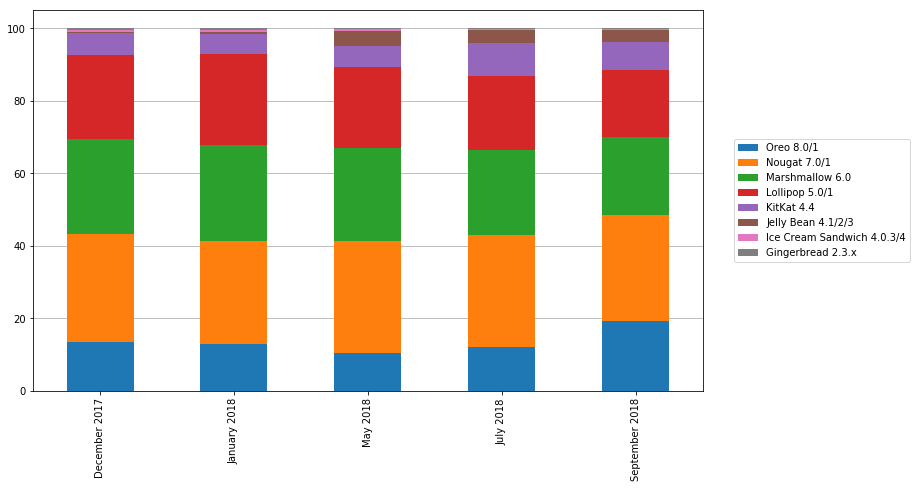
\includegraphics[keepaspectratio,width=0.8\textwidth]{AndroidMarketshare}
	\caption{Prozentanteil der Android Versionen, Daten von \cite{Fossbytes2018}}
	\label{fig:AndroidMarketshare}
\end{figure}


\newpage
\section{Systemspezifikation}
\label{sec:SysSpec}

\subsection{Anforderungen}
\label{ch:Anforderungen}
\begin{enumerate}
	\item Das Augmented Reality Objekt soll ausserhalb von Gebäuden ...
	\begin{enumerate}[label*=\arabic*.]
		\item mit einer maximale Abweichung von 10m auf einer minimalen Distanz von 50m bis zu einer Distanz von 1km auf korrekter Position dargestellt werden (fortan korrekte Position genannt).
		\item eine maximale Rotationsabweichung von \ang{25} aufweisen.
		\item einen maximalen Grössenunterschied von 5\% zum Original aufweisen.
		\item mit einer Maximalen Verzögerung (bei Bewegung) von <1 Sekunde reagieren.
		\item nach Beendigung von langsamen($<=$10km/s) Bewegungen der Kamera auf der korrekten Position bleiben.
		\item nach Beendigung von mittelmässig schnellen (>10km/s und $<=$20km/s) Bewegungen wieder auf korrekter Position dargestellt werden.
		\item nach Beendigungen von schnellen (>20km/s) Bewegungen nach einer erneuten Initialisierung wieder auf korrekter Position dargestellt werden.
		\item nur in einer Distanz bis mindestens 1km dargestellt werden (gilt auch für alle Informationen zum Objekt).
	\end{enumerate}
	\item Sobald das Objekt ausserhalb des Sichtfeldes ist, soll dem Benutzer eine Anzeige für das Wiederauffinden des Objektes angezeigt werden (basierend auf Kapitel \ref{ch:GraphicalUserInterface}).
	\item Sofern keine Informationen zur Lokalisierung vorhanden sind soll der Benutzer in weniger als 3 Sekunden über diese fehlende Informationen informiert werden (basierend auf Kapitel \ref{ch:GraphicalUserInterface}).
\end{enumerate}

\subsection{Kontext}
Das nachfolgende Kontextdiagramm (Abbildung \ref{fig:Kontext}) beschreibt die Interaktion der AR Applikation mit dem Benutzer, Systemen und anderen Prozessen. Es zeigt somit den Kontext der gesamten Applikation auf.

\begin{figure}[h!]
	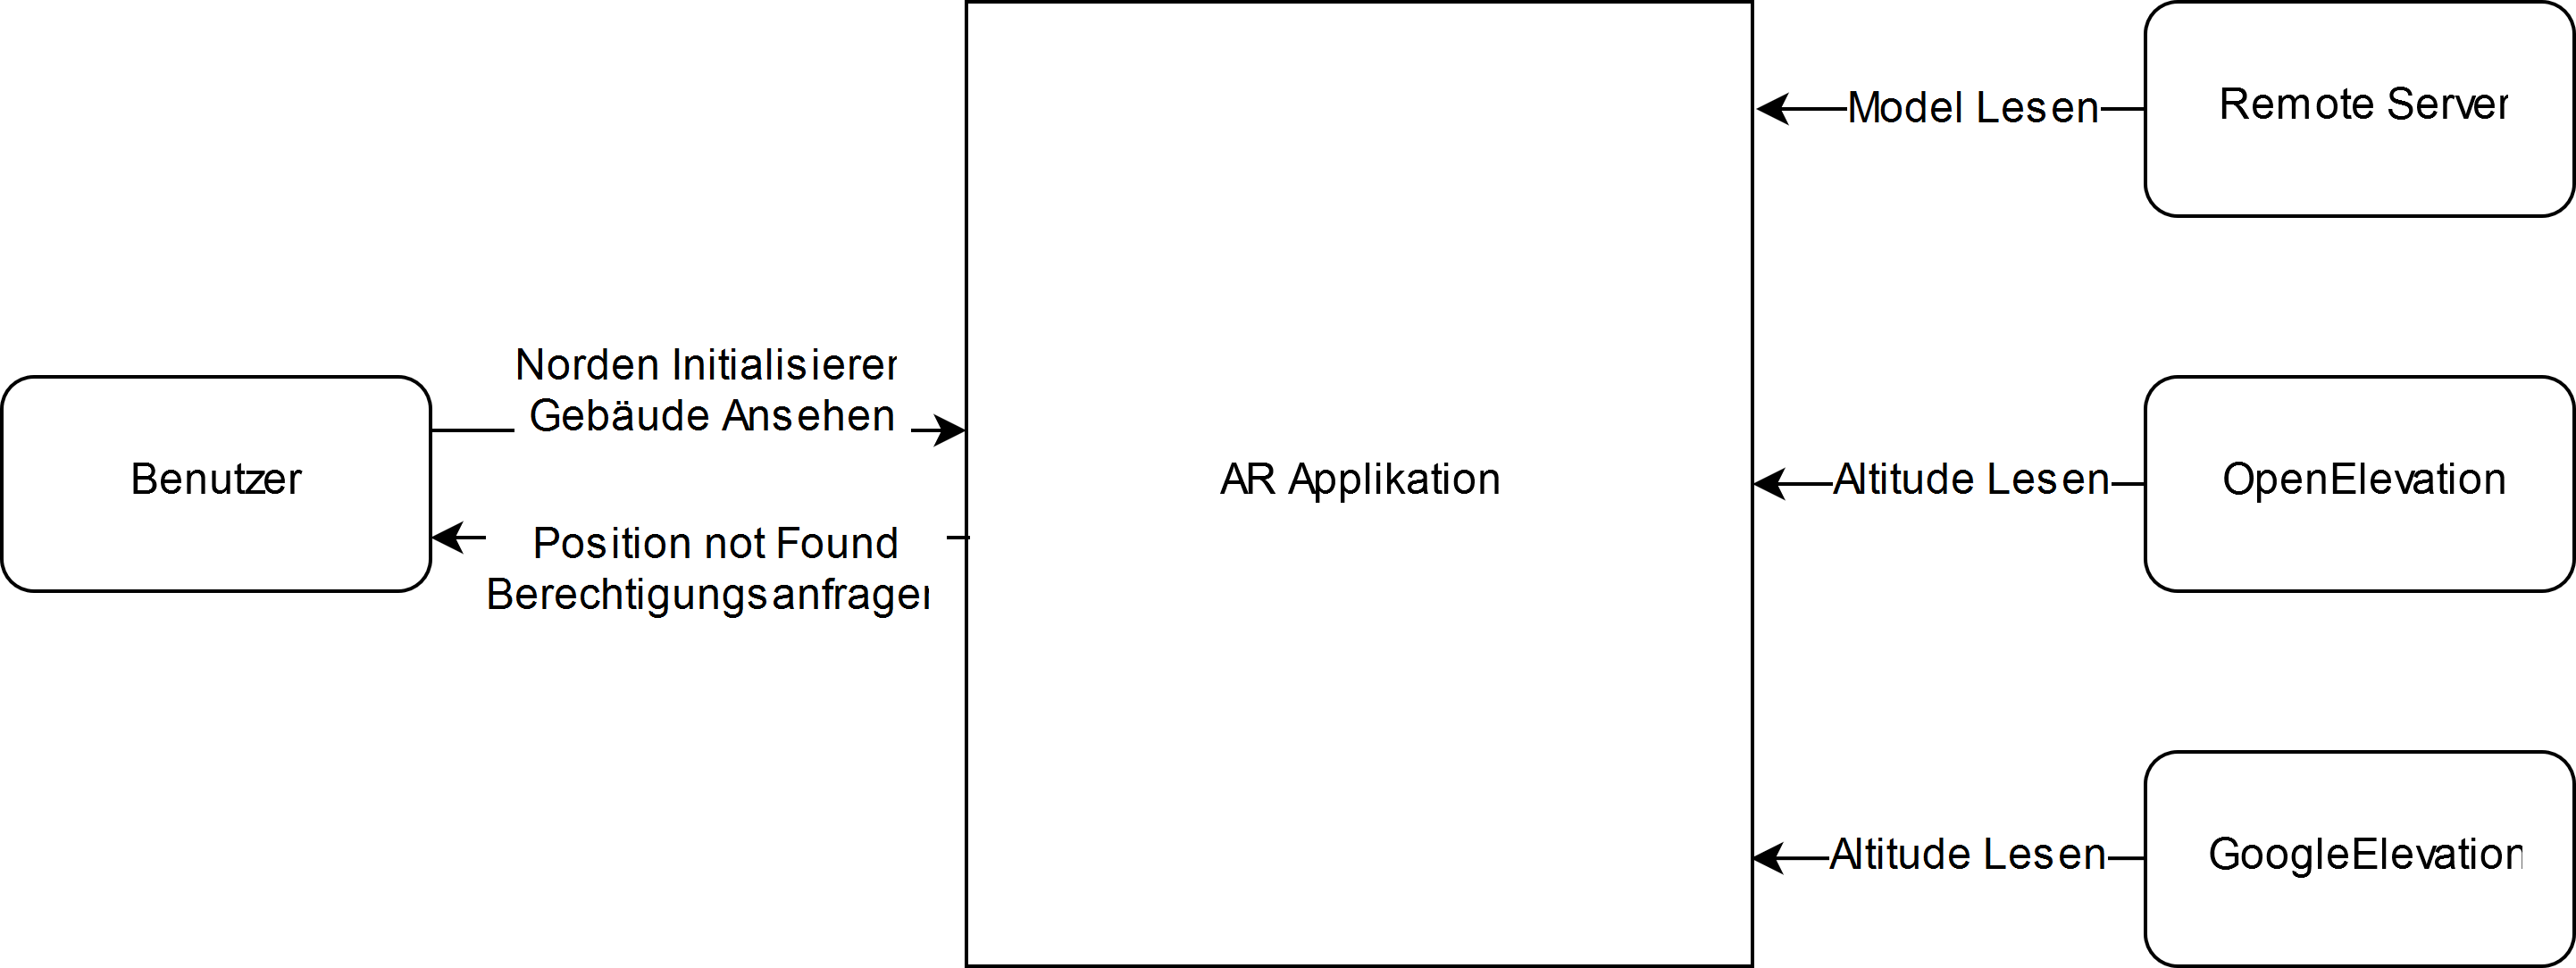
\includegraphics[keepaspectratio, width=\textwidth]{KontextDiagram.png}
	\caption{Kontextdiagramm}
	\label{fig:Kontext}
\end{figure}

\clearpage

\subsection{Komponentendesign}

Die entwickelte Applikation ist von weiteren Komponenten und Teilsystemen abhängig. In der Abbildung \ref{fig:Komponentendesign} sind nur die wichtigsten Komponenten, welche für die Funktionstüchtigkeit notwendig sind, abgebildet.
\bigbreak
Besonderer Augenmerk geht auf die GPS und OpenElevation Komponenten, da diese nicht auf dem Gerät selber sind und daher eine weitere Fehlerquelle (Funktionieren des externen Systems bedingen).

\begin{figure}[h!]
	\centering
	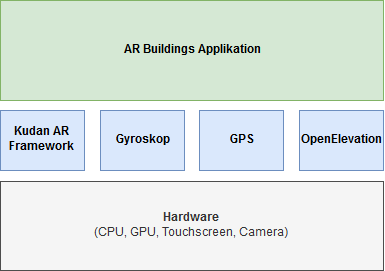
\includegraphics[width=0.7\linewidth, keepaspectratio]{Komponentendesign}
	\caption{Komponenten der ARBuildings Applikation}
	\label{fig:Komponentendesign}
\end{figure}

\subsubsection{Out of Scope}
Aus der Abbildung \ref{fig:Kontext} wird ersichtlich, dass die Applikation mit verschiedenen Systemen agiert. Das System Remote Server ist dabei ein geplanter Server, welcher die Modelle und deren Koordinaten enthält. Dieser Server ist nicht Bestandteil dieses Projektes und soll lediglich bei der Planung mit einbezogen werden.

\subsection{Architektur \& Design}
Die Architektur des Projektes wurde in 3 Schichten aufgeteilt. Diese werden in der nachfolgenden Grafik dargestellt.Dabei werden Abhängigkeiten untereinander wie auch zu externen Schnittstellen aufgezeigt.

\begin{figure}[h!]
	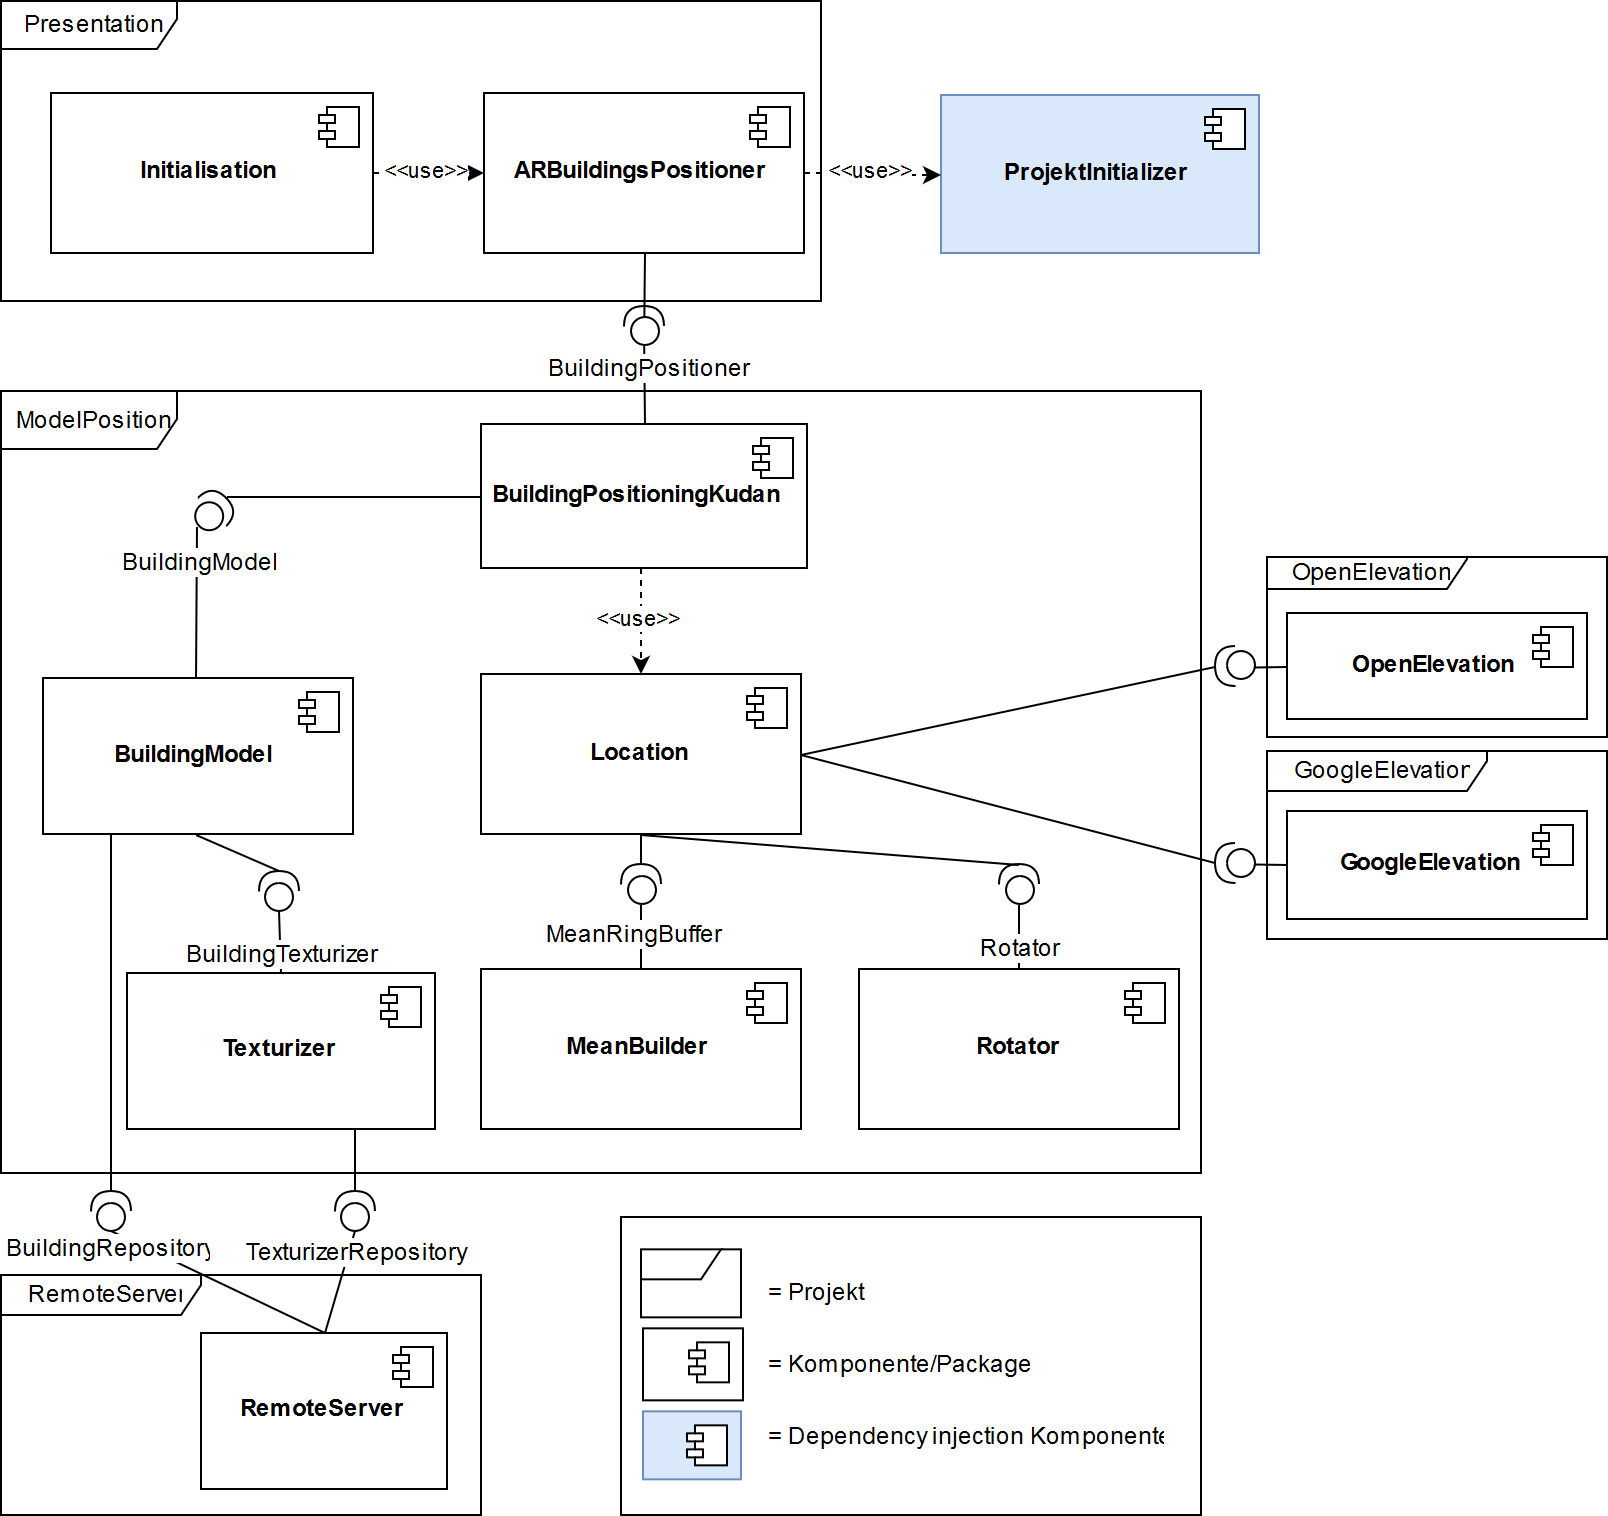
\includegraphics[keepaspectratio, width=\textwidth]{ArchitekturOverviewV0_5.png}
	\caption{Architekturübersicht}
\end{figure}

Eine detaillierte Beschreibung der einzelnen Schichten ist in den folgenden Kapiteln zu finden.

\begin{figure}[h!]
  \center
  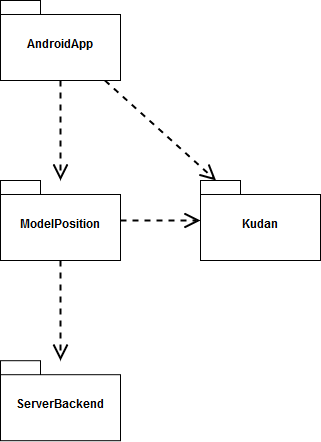
\includegraphics[width=0.35\textwidth]{SchichtenDiagramm.png}
  \caption{Übersicht der simplifizierten Schichtenarchitektur}
\end{figure}

\subsubsection{Presentation}
In Presentation befindet sich die kompletten grafischen Elemente der Applikation. Dies ist das Interface, mit welchem der User arbeitet. Zudem werden hier die benötigten Berechtigungen geprüft und wenn nötig vom Benutzer erfragt, sowie die Initialisierung gegen Norden gemacht. 

\subsubsection{ModelPosition}
In ModelPosition ist die gesamte Logik für die Positionierung eines Gebäudes in der virtuellen Kudan Welt enthalten. Es abstrahiert zudem die Zugriffe auf Kudan selber, sodass diese nicht in der eigentlichen AndroidApp Komponente zu finden sind.

\subsubsection{Server}
Der Server ist eine über eine REST Schnittstelle ansprechbare Komponente, welche das dynamische Laden von neuen Gebäuden ermöglicht. Diese ist ausserhalb dieses Projektscopes, wurde aus Gründen der Vollständigkeit jedoch dokumentiert und spezifiziert.

\subsection{Externe Schnittstellen}
Neben der Android Bibliothek wurde KudanAR als externe Schnittstelle verwendet. Die Dokumentation zu dieser Schnittstelle für Android ist unter folgendem Link zu finden:
\href{https://www.kudan.eu/docs-reference/AndroidDocs/annotated.html}{Dokumentation Kudan - Android}

Um die Höhe anhand der Koordinaten zu errechnen wurde sowohl die OpenElevation wie auch die GoogleMaps API angesprochen. Beide unterstützen eine Abfrage über eine GET-Abfrage und beide die gleiche Genauigkeit der Koordinaten, nämlich $0.000 001$ Grad. Was das Gradmass auf Meter übertragen bedeutet, wird in Tabelle \ref{tab:GradMeter} dargestellt. Dabei wird folgende Formel zu Hilfe genommen:

\indexequation{b = \frac{\pi}{\SI{180}{\degree}}\cdot\beta\cdot 6378.137}{Bogenlänge $b$ des Winkels $\beta$ mit Radius 6378.137m (Distanz zum Erdmittelpunkt am Äquator)}{Bogenlaenge}

Wie der Tabelle entnommen werden kann, entspricht die maximale Abweichung (angenommen die empfangenen Daten sind absolut korrekt) $0.05$ Meter. Um jedoch zusätzlich nicht einem Rate Limiting Opfer zu Fallen werden Abfragen auf $10^{-4}$ gerundet. Dies entspricht einer Abweichung von elf Metern, die Annahme ist dabei, dass die Höhe innerhalb dieser Distanz nicht sprunghaft ansteigt oder sinkt.

\begin{table}[htb]
	\centering
	\begin{tabular}{|c|c|}
		\hline
		\textbf{Differenz in \SI{}{\degree}} & \textbf{Differenz in Metern}\\
		\hline
		0.1 & 11131.94908 \\
		\hline
		0.01 & 1113.194908 \\
		\hline
		0.001 & 111.3194908 \\
		\hline
		0.000 1 & 11.13194908 \\
		\hline
		0.000 01 & 1.113194908 \\
		\hline
		0.000 001 & 0.111319491 \\
		\hline
	\end{tabular} 
	\caption{Auswirkung einer Gradeinteilung in Metern, dabei ist die Annahme, dass die Erde eine perfekte Sphäre ist}
	\label{tab:GradMeter}
\end{table}

\subsection{Interne Schnittstellen}

\subsubsection{Building Positioner}
Die BuildingPositioner Schnittstelle ist verantwortlich für die Abstraktion des gesamten Positionierungsprozesses zur Applikation. Es bietet zudem Methoden an, welche dem Starten und Stoppen des Prozesses dienen.
\begin{figure}[h!]
	\center
	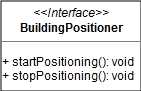
\includegraphics[scale=0.6]{BuildingPositioner.png}
	\caption{BuildingPositioner Interface}
\end{figure}
\clearpage
\subsubsection{Building Model}
Das Building Model Interface ist das Bindeglied zwischen der realen Position des Benutzers und der virtuellen Position in der Applikationswelt. Es ist dafür verantwortlich, dass das Gebäude reale Positionsdaten besitzt und die virtuellen Koordinaten an das Modell in der virtuellen Welt übergibt.

\begin{figure}[h!]
	\center
	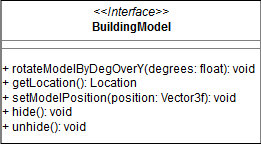
\includegraphics[scale=0.6]{BuildingModel.png}
	\caption{Building Model Interface}
\end{figure}

\subsubsection{Building Texturizer}
Der BuildingTexturizer ist verantwortlich für die Einfärbung des Modelles.
\begin{figure}[h!]
	\center
	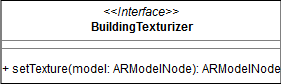
\includegraphics[scale=0.6]{BuildingTexturizer.png}
	\caption{Texturizer Interface}
\end{figure}


\subsubsection{Rotator}
Der Rotator verpflichtet sich ein Rotating Object in einem Raum, um eine bestimmte Achse zu drehen.
\begin{figure}[h!]
	\center
	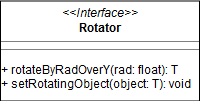
\includegraphics[scale=0.6]{Rotator.png}
	\caption{Rotator Interface}
\end{figure}


\subsubsection{Mean Ring Buffer}
Der Mean Ring Buffer ist verantwortlich, dass ein Mittelwert eines Objektes <T> aus den übergebenen Objekten berechnet wird.
\begin{figure}[h!]
	\center
	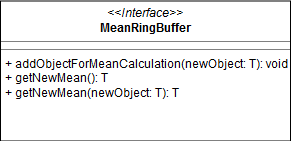
\includegraphics[scale=0.6]{MeanRingBuffer.png}
	\caption{Mean ring buffer Interface}
\end{figure}

\subsubsection{Async Elevation Request Callee}
Das AsyncElevationRequestCallee abstrahiert die Rückgabemethode für einen AsyncElevationRequest.
\begin{figure}[h!]
	\center
	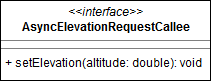
\includegraphics[scale=0.6]{AsyncElevationRequestCallee.png}
	\caption{AsyncElevationRequestCallee Interface}
\end{figure}

\subsection{Klassendiagramm}
Nachfolgend ist das Klassendiagramm der AR Applikation. Es zeigt die Packages auf und deren Klassen. Zusätzlich ist auf Serverseite eine REST API angedacht.

\begin{figure}[h!]
	\center
	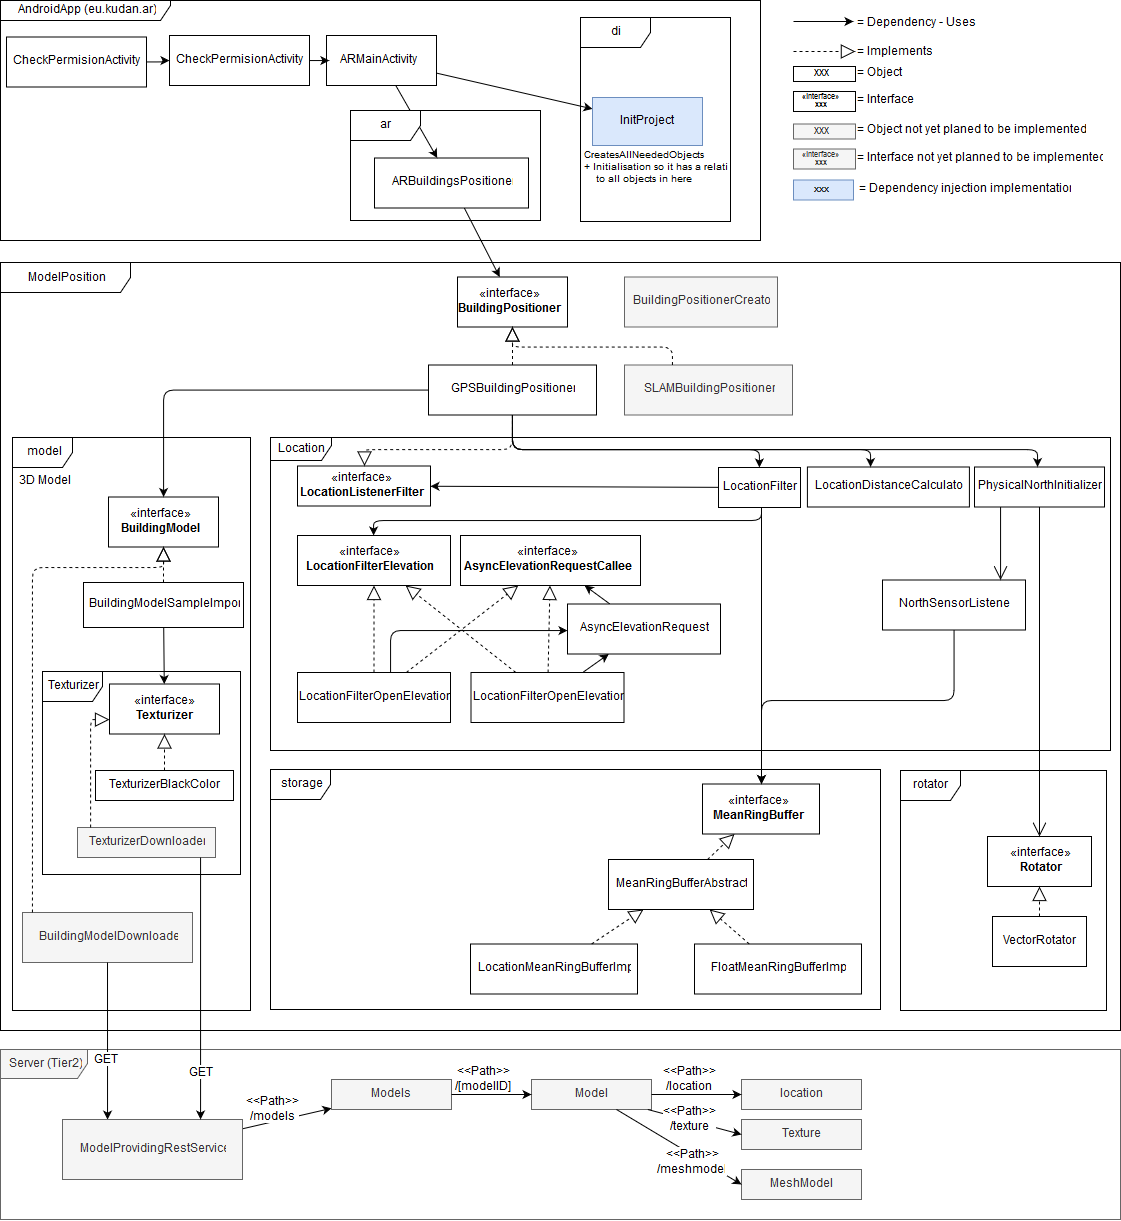
\includegraphics[width=\textwidth]{Klassendiagramm.png}
	\caption{Klassendiagramm der AR Applikation}
\end{figure}


\subsection{Anforderungen der Software}

\subsubsection{Hardware}

Die AR Applikation stellte folgende Hardware Anforderungen an das Gerät:

\begin{enumerate}
	\item Lokalisierungssensor
	\item Kompass
	\item Gyroskop
\end{enumerate}

\subsubsection{Software}

Die AR Applikation stellt zudem folgende Software Anforderungen an das Gerät:

\begin{itemize}
	\item Android OS (mindestens Version 6.0)
	\item Aktive Internetverbindung
\end{itemize}

\subsection{Umsetzung Programmierung}

\subsubsection{Clean Code}

Da gut lesbarer Code verständlicher und zeitnaher die Aufgaben des Codes widerspiegelt als ein Kommentar, wurde grösstenteils auf JavaDoc und weitere Kommentare verzichtet. Dies hatte zur Folge, dass bei der Erstellung einer Methode notwendigerweise ein selbst sprechender Name für diese sowie deren Parameter gewählt werden musste.

\subsubsection{Git Flow}

Um möglichst effizient und unabhängig voneinander zu programmieren, sowie zu dokumentieren, wurde mit Git Feature Branch Workflow gearbeitet. Dies bedeutet, dass für jedes Feature einen Branch erstellt wurde (\cite{gitFeatureBranchWorkflow}). Weiter wurde eine Regelung eingeführt, wobei ein Branch nicht vom Ersteller in den Master Branch zusammengeführt werden darf. Dies schafft Sicherheit, da eine zweite Person einen Review des Codes macht.
Auf der Abbildung \ref{fig:FeatureBranchWorkflow} ist ein Auszug aus der Baumstruktur unserer Dokumentation dargestellt. Dabei ist zu erkennen, dass zu Sprintbeginn möglichst keine offenen Zweige (engl. Branches) mehr vorhanden sind und gegen Sprintende alle Zweige in den Master (in Abbildung \ref{fig:FeatureBranchWorkflow} schwarz dargestellt) über einen Pull Request zusammengeführt werden.

\begin{figure}[h!]
	\center
	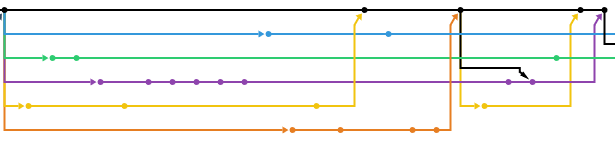
\includegraphics[width=\textwidth]{GitFeatureBranchWorkflow.png}
	\caption{Branches unsere Dokumentation aus Sprint 5}
	\label{fig:FeatureBranchWorkflow}
\end{figure}

\subsubsection{Unit Test}
Da es sich bei der entwickelten Applikation um einen Prototyp handelt, wurde zu Beginn des Projektes entschlossen, die Anzahl an Unit Tests vorerst noch gering zu halten. Dies ermöglichte, dass wir genug Zeit hatten um verschiedene Prototypen zu entwickeln.

\section{Testing}

\subsection{Testfälle}
Basierend auf den Anforderungen, welche in Kapitel \ref{ch:Anforderungen} definiert sind, wurden verschiedene Tests erstellt. In Kapitel \ref{ch:testprotokoll} ist das Protokoll zu diesen Tests zu finden. Die Testfälle werden mit einer Version versehen. Alte Testfälle sind im git Repository weiterhin verfügbar.

\subsubsection{Testfall 1-Berechtigung erlauben}
\begin{tabularx}{\textwidth}{|l|X|}
\hline
	Version &
	T-001v1 \\
\hline
	Beschreibung & Berechtigungsanfragen \\
\hline
	Testvoraussetzung & Die App hat die Berechtigungen noch nicht. \\
\hline
	Testschritte &
		1. App starten \\ &
		2. Berechtigungen erteilen \\
\hline
	Erwartetes Ergebnis & Nachdem alle Berechtigungen erteilt wurden, startet die App normal -> der North Initialize Bildschirm erscheint. \\
\hline
\end{tabularx}
\subsubsection{Testfall 2-Berechtigung verweigern}
\begin{tabularx}{\textwidth}{|l|X|}
\hline
	Version &
	T-002v1 \\
\hline
	Beschreibung & Berechtigungsanfragen verweigern \\
\hline
	Testvoraussetzung & Die App hat die Berechtigungen noch nicht. \\
\hline
	Testschritte &
		1. App starten \\ &
		2. Berechtigungsanfragen sehen und ablehnen \\
\hline
	Erwartetes Ergebnis & Nachdem alle Berechtigungen abgelehnt wurden, bleibt die App in einem Abfangbildschirm, wo die Nachfrage für die Berechtigungen erneut gestartet werden kann. \\
\hline
\end{tabularx}
\subsubsection{Testfall 3-Starten von Kudan}
\begin{tabularx}{\textwidth}{|l|X|}
\hline
	Version &
	T-003v2 \\
\hline
	Beschreibung &
	Es soll überprüft werden ob die Kudan Komponenten starten.\\
\hline
	Testvoraussetzung &
	T-001 wurde durchgeführt (Berechtigungen erhalten). \\
\hline
	Testschritte &
		1. App starten \\ &
		2. Gerät nach Norden ausrichten \\
\hline
	Erwartetes Ergebnis &
	Es soll der Kamerabildschirm angezeigt werden. \\
\hline
\end{tabularx}
\subsubsection{Testfall 4-Darstellung des Gebäudes Ausrichtung Norden}
\begin{tabularx}{\textwidth}{|l|X|}
\hline
	Version &
	T-004v2 \\ 
\hline 
	Beschreibung & 
	Bei diesem Testfall soll getestet werden, ob das Gebäude dargestellt wird. \\ 
\hline 
	Testvoraussetzung &
	Die App ist auf dem Smartphone installiert. GPS gemocked auf folgende Position: \\ & 
		47.145739885261925,8.436641571608824, Altitude: 450 \\ 
\hline 
	Testschritte & 
		1. Smartphone nach Norden ausrichten\\ &
		2. App starten\\ &
		3. Smartphone erneut nach Norden ausrichten\\ &
		4. Initialisierung abwarten (ca. 3 Sekunden)\\
\hline
	Erwartetes Ergebnis &
	Das Gebäude wird auf 7Uhr 30 dargestellt. \\
\hline
\end{tabularx}
\subsubsection{Testfall 5-Darstellung des Gebäudes Ausrichtung Westen}
\begin{tabularx}{\textwidth}{|l|X|}
\hline
	Version &

	T-005v2 \\ 
\hline 
	Beschreibung & 
	Bei diesem Testfall soll getestet werden, ob das Gebäude dargestellt wird, wenn es nicht nach Norden gerichtet ist. \\ 
\hline 
	Testvoraussetzung &
	Die App ist auf dem Smartphone installiert. GPS gemocked auf folgende Position: \\ &
		47.145739885261925,8.436641571608824, Altitude: 450 \\ 
\hline 
	Testschritte & 
		1. Smartphone nach Westen ausrichten\\ &
		2. App starten\\ &
		3. Smartphone nach Norden ausrichten\\
\hline
	Erwartetes Ergebnis &
	Das Gebäude wird auf 7Uhr 30 dargestellt\\ 
\hline 
\end{tabularx}
\subsubsection{Testfall 6-Darstellung Gebäude mit Bewegung nach rechts}
\begin{tabularx}{\textwidth}{|l|X|}
\hline
	Version &
	T-006v2 \\
\hline
	Beschreibung &
	Bei diesem Testfall soll getestet werden, ob das Gebäude dargestellt wird und sich die Position des Gebäudes den GPS Daten anpasst. \\
\hline
	Testvoraussetzung &
	Die App ist auf dem Smartphone installiert. GPS gemocked auf folgende Position: \\ &
		47.145739885261925,8.436641571608824, Altitude: 450 \\ 
\hline 
	Testschritte & 
		1. Smartphone nach Westen ausrichten\\ &
		2. App starten\\ &
		3. Smartphone nach Norden ausrichten\\ &
		4. App minimieren (Home Button drücken)\\ &
		5. GPS Mocklocation verändern (auf Position 47.145739885261925,8.436641571608824)\\ &
		6. App erneut öffnen\\
\hline
	Erwartetes Ergebnis &
	Das Gebäude wandert von 7Uhr 30 auf 9Uhr.\\ 
\hline
\end{tabularx}
\subsubsection{Testfall 7-Darstellung Gebäude mit Bewegung nach links}
\begin{tabularx}{\textwidth}{|l|X|}
\hline
	Version &
	T-007v2 \\
\hline
	Beschreibung &
	Bei diesem Testfall soll getestet werden, ob das Gebäude dargestellt wird und sich die Position des Gebäudes den GPS Daten anpasst. \\
\hline
	Testvoraussetzung &
	Die App ist auf dem Smartphone installiert. GPS gemocked auf folgende Position: \\ &
		47.142958, 8.430126, Altitude: 450 \\ 
\hline 
	Testschritte & 
		1. Smartphone nach Norden ausrichten\\ &
		2. App starten\\ &
		3. Smartphone nach Norden ausrichten\\ &
		4. App minimieren (Home Button drücken)\\ &
		5. GPS Mocklocation verändern (auf Position  47.141427, 8.432621)\\ &
		6. App erneut öffnen\\
\hline
	Erwartetes Ergebnis &
	Das Gebäude wandert von 15Uhr auf 12Uhr. \\ 
\hline 
\end{tabularx}
\subsubsection{Testfall 8-Entfernen der Berechtigung zur Laufzeit}
\begin{tabularx}{\textwidth}{|l|X|}
\hline
	Version &
	T-008v1 \\ 
\hline 
	Beschreibung & 
	Bei diesem Testfall so überprüft werden, ob die App nicht abstürzt, wenn zur Laufzeit der App Berechtigungen entzogen werden. \\ 
\hline 
	Testvoraussetzung &
	Die App ist auf dem Smartphone installiert und hat alle nötigen Berechtigungen. \\ 
\hline 
	Testschritte & 
		1. App starten\\ &
		2. App minimieren\\ &
		3. Berechtigungen der App entfernen\\ &
		4. App wieder öffnen\\
\hline
	Erwartetes Ergebnis &
	Die App wechselt wieder auf den Berechtigungsbildschirm. \\
\hline
\end{tabularx}
\subsubsection{Testfall 9-Smartphone Rotation}
\begin{tabularx}{\textwidth}{|l|X|}
\hline
	Version &
	T-009v2 \\
\hline
	Beschreibung &
	Es soll überprüft werden wie das Verhalten ist, wenn das Smartphone rotiert wird. \\
\hline
	Testvoraussetzung &
	Die App hat alle Berechtigungen. \\ 
\hline 
	Testschritte & 
		1. App starten\\ &
		3. Smartphone nach Norden ausrichten\\ &
		3. Rotieren des Smartphones um 90 Grad (Portrait auf Landscape)\\
\hline
	Erwartetes Ergebnis &
	Die App soll keine Rotationsanimation beinhalten. Die App soll das Gebäude weiter anzeigen. \\
\hline
\end{tabularx}
\subsubsection{Testfall 10-Spezialtest Überprüfung mittels Gebäude}
\begin{tabularx}{\textwidth}{|l|X|}
\hline
	Version &
	T-010v1 \\ 
\hline 
	Beschreibung & 
	Es soll überprüft werden, ob das bestehende Gebäude mit dem AR Gebäude deckungsgleich ist. \\ 
\hline 
	Testvoraussetzung &
	Die App hat alle Berechtigungen\\ &
	Teil des Gebäudekomplexes ist sichtbar\\ &
	Der Tester befindet sich vor Ort\\ 
\hline 
	Testschritte & 
		1. Tester läuft auf Position (47.142835, 8.431436)\\ &
		2. App starten\\ &
		3. Smartphone nach Norden ausrichten\\ &
		4. Gebäudekomplex in Kamera fokussieren\\
\hline
	Erwartetes Ergebnis &
	Die App soll das AR Modell über dem Realen Gebäude darstellen. \\ &
	Randbedingungen: \\ &
		Maximale Abweichung 10m in alle Richtungen.\\
\hline
\end{tabularx}
\subsubsection{Testfall 11-Grössenunterschied}
\begin{tabularx}{\textwidth}{|l|X|}
\hline 
	Version &
	T-011v1 \\ 
\hline 
	Beschreibung & 
	Es soll überprüft werden, ob die Grösse des bestehenden Gebäudes mit dem AR Gebäude deckungsgleich ist. \\ 
\hline
    Testvoraussetzung &
	Die App hat alle Berechtigungen.\\ &
	Teil des Gebäudekomplexes ist sichtbar.\\ &
	Der Tester befindet sich vor Ort. \\ &
	Das Gebäude wird nach Initialisierung an korrekter Position dargestellt. \\
\hline 
	Testschritte & 
		1. Tester läuft auf Position (47.142835, 8.431436)\\ &
		2. App starten\\ &
		3. Smartphone nach Norden ausrichten\\ &
		4. Gebäudekomplex in Kamera fokussieren. \\
\hline
	Erwartetes Ergebnis &
	Die App soll das AR Modell über dem realen Gebäude darstellen. \\ &
	Randbedingungen: \\ &
		Der maximale Grösssenunterschied beträgt < 5\% (Augenmass). \\ 
\hline 
\end{tabularx}
\subsubsection{Testfall 12-Rotationsabweichung}
\begin{tabularx}{\textwidth}{|l|X|}
\hline 
	Version &
	T-012v1 \\ 
\hline 
	Beschreibung & 
	Es soll überprüft werden, ob das bestehende Gebäude mit dem AR Gebäude betreffend Rotation deckungsgleich ist. \\ 
\hline 
	Testvoraussetzung &
	Die App hat alle Berechtigungen. \\ &
	Teil des Gebäudekomplexes ist sichtbar. \\ &
	Der Tester befindet sich vor Ort. \\ &
	Das Gebäude wird nach Initialisierung an korrekter Position dargestellt. \\
\hline 
	Testschritte & 
		1. Tester läuft auf Position (47.142835, 8.431436)\\ &
		2. App starten\\ &
		3. Smartphone nach Norden ausrichten\\ &
		4. Gebäudekomplex in Kamera fokussieren\\
\hline
	Erwartetes Ergebnis &
	Die App soll das AR Modell über dem Realen Gebäude darstellen. \\ &
	Randbedingungen: \\ &
		Der maximale Rotationsabweichung beträgt < \ang{25} (Augenmass). \\ 
\hline 
\end{tabularx}

\subsubsection{Testfall 13-Leichte bis starke Erschütterung}
\begin{tabularx}{\textwidth}{|l|X|}
\hline 
	Version &
	T-013v1 \\ 
\hline 
	Beschreibung & 
	Es soll überprüft werden, ob das bestehende Gebäude mit dem AR Gebäude deckungsgleich bleibt, nachdem das Smartphone leichten bis starken Erschütterungen ausgesetzt war. \\ 
\hline 
	Testvoraussetzung &
	Die App hat alle Berechtigungen. \\ &
	Teil des Gebäudekomplexes ist sichtbar. \\ &
	Der Tester befindet sich vor Ort. \\ &
	Das Gebäude wird nach Initialisierung an Korrekter Position dargestellt. \\
\hline 
	Testschritte & 
		1. Tester läuft auf Position (47.142835, 8.431436) \\ &
		2. App starten\\ &
		3. Smartphone nach Norden ausrichten\\ &
		4. Gebäudekomplex in Kamera fokussieren\\ &
		5. Leichte / Mittlere / Starke Erschütterung simulieren\\
\hline
	Erwartetes Ergebnis &
	Die App soll das AR Modell wieder an derselben Position darstellen.\\ 
\hline 
\end{tabularx}

\subsubsection{Testfall 14-Darstellungsgeschwindigkeit}
\begin{tabularx}{\textwidth}{|l|X|}
\hline 
	Version &
	T-014v1 \\ 
\hline 
	Beschreibung & 
	Es soll überprüft werden, ob das AR Gebäude schnell auf die Smartphone-Bewegungen reagiert. \\ 
\hline 
	Testvoraussetzung &
	Die App hat alle Berechtigungen \\ &
	Teil des Gebäudekomplexes ist sichtbar \\ &
	Der Tester befindet sich vor Ort \\ &
	Das Gebäude wird nach Initialisierung an korrekter Position dargestellt. \\
\hline 
	Testschritte & 
		1. Tester läuft auf Position (47.142835, 8.431436) \\ &
		2. App starten \\ &
		3. Smartphone nach Norden ausrichten\\ &
		4. Gebäudekomplex in Kamera fokussieren\\ &
		5. Leichte bewegungen des Smartphones\\
\hline
	Erwartetes Ergebnis &
	Die App soll das AR Modell ohne Verzögerungen über einer Sekunde darstellen. \\ 
\hline 
\end{tabularx}


\subsubsection{Testfall 15-Darstellung bis mindestens 1km Entfernung}
\begin{tabularx}{\textwidth}{|l|X|}
\hline 
	Version &
	T-015v1 \\ 
\hline 
	Beschreibung & 
	Es soll überprüft werden, ob das AR Gebäude bis mindestens 1km Entfernung dargestellt wird. \\ 
\hline 
	Testvoraussetzung &
	Die App hat alle Berechtigungen \\ &
	Teil des Gebäudekomplexes ist Sichtbar \\ &
	Der Tester befindet sich vor Ort \\ &
	Das Gebäude wird nach Initialisierung an korrekter Position dargestellt. \\
\hline 
	Testschritte & 
		1. Tester läuft auf Position (47.135743, 8.425906) \\ &
		2. App starten \\ &
		3. Smartphone nach Norden ausrichten\\ &
		4. Gebäudekomplex in Kamera fokussieren\\ 
\hline
	Erwartetes Ergebnis &
	Die App soll das AR Modell in der Distanz Darstellen \\ 
\hline 
\end{tabularx}
\subsection{Testprotokoll}
\label{ch:testprotokoll}
Die folgende Tabelle zeigt ob die Tests erfolgreich waren oder nicht. Genauere Resultate sind im Anhang \ref{appendig:testprotokolle} zu finden . 
\bigbreak

\begin{tabularx}{\textwidth}{|l|X|l|}
\hline
	\textbf{TestID/Version }& \textbf{Beschreibung} & \textbf{Passed} \\
\hline
	T-001v1 & Berechtigungsanfragen & \checkmark \\
\hline
	T-002v1 & Berechtigungsanfragen verweigern & \checkmark \\
\hline
	T-003v2 & Es soll überprüft werden ob die Kudan Komponenten starten. & \checkmark \\
\hline
	T-004v2 & Bei diesem Testfall soll getestet werden, ob das Gebäude dargestellt wird. & \checkmark \\
\hline
	T-005v2 & Bei diesem Testfall soll getestet werden, ob das Gebäude dargestellt wird, wenn es nicht nach norden gerichtet ist. & \checkmark \\
\hline
	T-006v2 & Bei diesem Testfall soll getestet werden, ob das Gebäude dargestellt wird und sich die Position des Gebäudes den GPS Daten anpasst. & \checkmark \\
\hline
	T-007v2 & Bei diesem Testfall soll getestet werden, ob das Gebäude dargestellt wird und sich die Position des Gebäudes den GPS Daten anpasst. & \checkmark \\
\hline
	T-008v1 & Bei diesem Testfall so überprüft werden ob die App nicht abstürzt, wenn zur Laufzeit der App Berechtigungen entzogen werden. & \checkmark \\
\hline
	T-009v2 & Es soll überprüft werden wie das Verhalten ist, wenn das Smartphone rotiert wird. & \checkmark \\
\hline
	T-010v1 & Es soll überprüft werden, ob das bestehende Gebäude mit dem AR Gebäude deckungsgleich ist. & x \\
\hline
	T-011v1 & Es soll überprüft werden, ob das bestehende Gebäude mit dem AR Gebäude deckungsgleich was die Grösse des Gebäudes betrifft. & \checkmark \\
\hline
	T-012v1 & Es soll überprüft werden, ob das bestehende Gebäude mit dem AR Gebäude deckungsgleich was die Rotation des Gebäudes betrifft. & \checkmark \\
\hline
	T-013v1 & Es soll überprüft werden, ob das bestehende Gebäude mit dem AR Gebäude deckungsgleich bleibt, nachdem das Smartphone leichten bis starken Erschütterungen ausgesetzt war. & \checkmark \\
\hline
	T-014v1 & Es soll überprüft werden, ob das AR Gebäude schnell auf die Smartphone-Bewegungen Reagiert. & \checkmark \\
\hline
	T-015v1 & Es soll überprüft werden, ob das AR Gebäude bis mindestens 1km Entfernung dargestellt wird. & \checkmark \\
\hline
\end{tabularx}

\chapter{Projektmanagementplan}

\section{Projektorganisation}
Da beide Projektmitglieder ihre Kompetenzen eher in den technischen Bereichen dieses Projekts sehen, wurde von einer strikten Aufgabenteilung abgesehen.

Es wurde dennoch darauf geachtet, dass beide Mitglieder klare Verantwortungen übernehmen. Diese waren jedoch mehr in einer überwachenden Funktion gesehen, und sollen nicht bedeuten, dass dieses Mitglied die Arbeit alleine leistete.

\vspace{1em}

\begin{tabularx}{\textwidth}{|X|X|}
	\hline
	\textbf{Teammitglied} & \textbf{Funktionen} \\
	\hline
	Pascal Baumann & \tabitem Dokumentation \\
	& \tabitem Testplanung \& Durchführung \\
	& \tabitem Projektmanagement \\
	\hline
	Dane Wicki & \tabitem Architektur \\
	& \tabitem Plattformanalyse \\
	\hline
\end{tabularx}

\newpage
\section{Projektführung}

\section{Rahmenplan}

Das Projekt wurde in 6 zweiwöchige Sprints unterteilt und in diesen iterativ entwickelt.

\vspace{1em}

\begin{figure}[h!]
	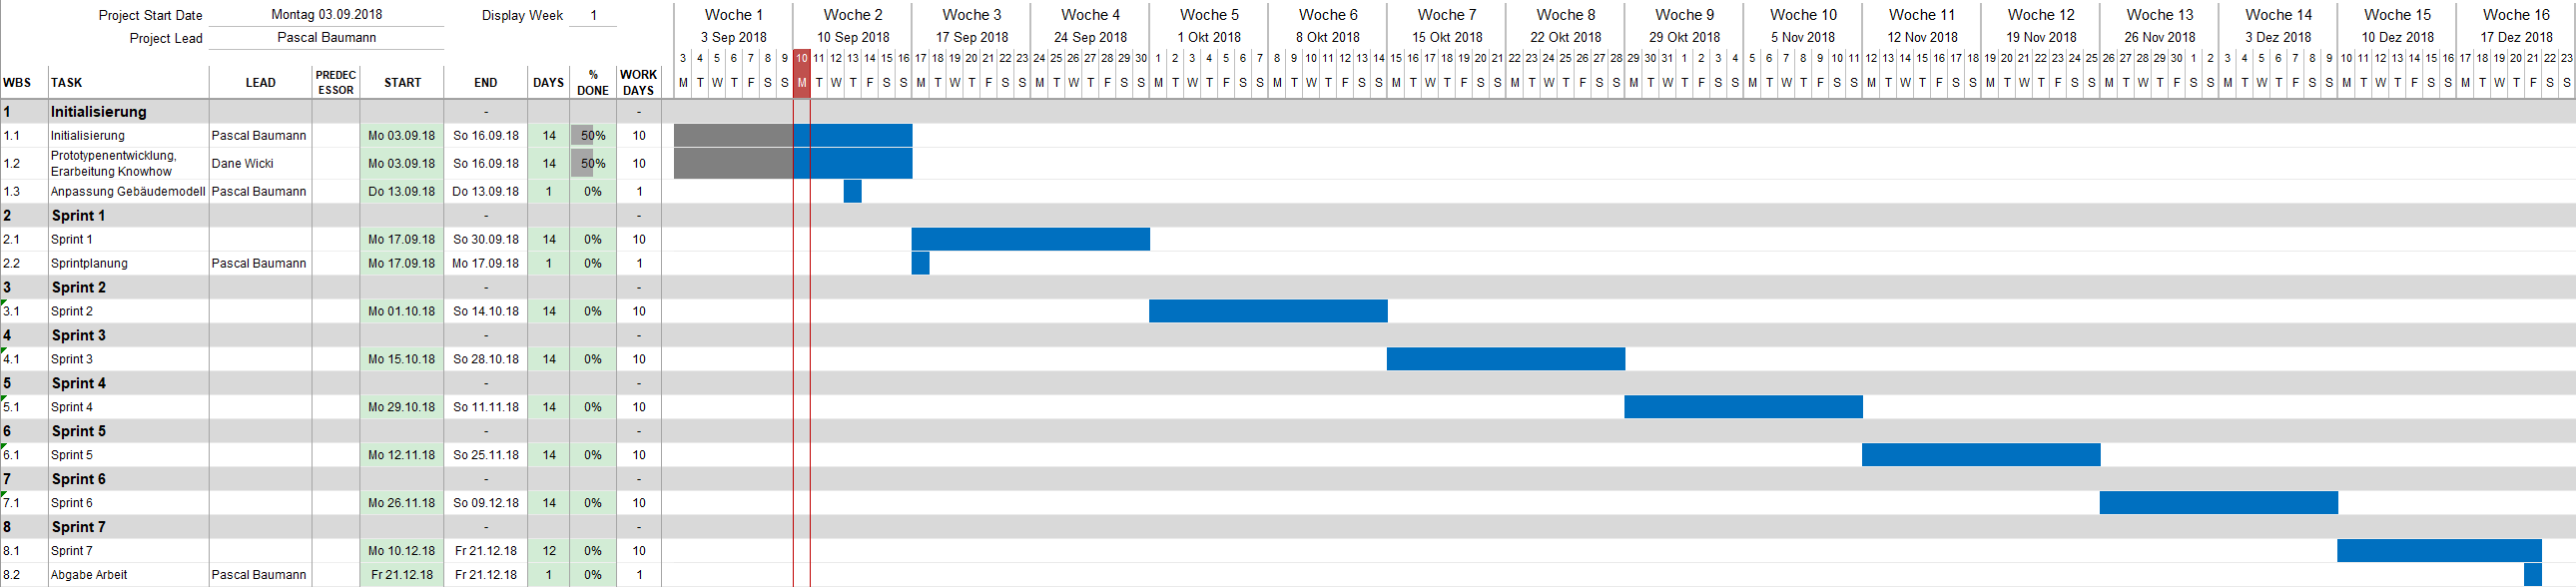
\includegraphics[keepaspectratio, width=\textwidth]{Rahmenplan}
	\caption{Überblick der Sprints}
\end{figure}

\section{Tools}
\label{sec:Tools}
\subsection{Entwicklung}
\begin{table}[h!]
	\begin{tabular}{p{0.5\textwidth} p{0.5\textwidth}}
		\hline
		\textbf{Tool} & \textbf{Version} \\
		\hline
		AndroidStudio & 3.2.1 \\
		\hline
		Blender & 2.79b \\
		\hline
		Unity (Prototypen) & 2018.2.15f1 \\
		\hline
	\end{tabular}
	\caption{Verwendete Versionen der Tools}
\end{table}

\subsection{Versions Kontrolle}
\begin{table}[h!]
	\begin{tabular}{p{0.5\textwidth} p{0.5\textwidth}}
		\hline
		\textbf{Tool} & \textbf{Version} \\
		\hline
		GitKraken & 4.1.1 \\
		\hline
		git & 2.19.2 \\
		\hline
		GitHub & GitHub.com \\
		\hline
	\end{tabular}
	\caption{Verwendete Versionen der Versionierungssysteme}
\end{table}

\clearpage
\subsection{Dokumentation}
\begin{table}[h!]
	\begin{tabular}{p{0.5\textwidth} p{0.5\textwidth}}
		\hline
		\textbf{Tool} & \textbf{Version} \\
		\hline
		MiKTex & 2.9.6821 \\
		\hline
		Mendeley Desktop & 1.19.2 \\
		\hline
		MS Excel & 11001.20108 \\
		\hline
		Mendeley & - \\
		\hline
		OneDrive & - \\
		\hline
	\end{tabular}
	\caption{Verwendete Versionen der Hilfsmittel für die Dokumentation}
\end{table}

\subsection{Frameworks}
\begin{table}[h!]
	\begin{tabular}{p{0.5\textwidth} p{0.5\textwidth}}
		\hline
		\textbf{Framework} & \textbf{Version} \\
		\hline
		Kudan Android SDK & 1.5.2 \\
		\hline
		Vuforia Unity (Prototypen) & 7.5.26 \\
		\hline
	\end{tabular}
	\caption{Verwendete Versionen der Frameworks}
\end{table}



\subsection{Repositories}
\begin{table}[h!]
	\begin{tabular}{p{0.5\textwidth} p{0.5\textwidth}}
		\hline
		\textbf{Name} & \textbf{URL} \\
		\hline
		AR-Building (Applikation) & \url{https://github.com/PAWI-HS18-ARBuilding/AR_Buildings} \\
		\hline
		Dokumentation & \url{https://github.com/PAWI-HS18-ARBuilding/Dokumentation} \\
		\hline
	\end{tabular}
	\caption{Verwendete Repositories}
\end{table}

\subsection{Übrige}
\begin{table}[h!]
	\begin{tabular}{p{0.5\textwidth} p{0.5\textwidth}}
		\hline
		\textbf{Tool} & \textbf{Verwendung} \\
		\hline
		Trello & Aufgabenverwaltung \\
		\hline
		WhatsApp & Kommunikation im Team \\
		\hline
	\end{tabular}
	\caption{Übrige Hilfsmittel}
\end{table}

\section{Risikomanagement}

Es werden mögliche Risiken, welche während dem Projekt auftreten können aufgezählt. Diese werden auf Eintrittswahrscheinlichkeit und Schadensmass eingeschätzt, danach wird entschieden, welche Massnahmen getroffen werden können, und was deren Auswirkungen sind.

\subsection{Definitionen}
\label{sssec:Def}
\vspace{1em}
\noindent
Eintrittswahrscheinlichkeit:

\vspace{1em}
\noindent
\begin{tabularx}{\textwidth}{|l|l|X|}
	\hline
	\textbf{Stufe} & \textbf{Bezeichnung} & \textbf{Beschreibung} \\
	\hline
	1 & unvorstellbar & Möglich aber eher unwahrscheinlich. Tritt nie oder einmal in 14 Wochen auf \\
	\hline
	2 & unwahrscheinlich & Kann in 14 Wochen 0-1 Mal eintreten\\
	\hline
	3 & vorstellbar & Kann in 14 Wochen 1-2 Mal eintreten \\
	\hline
	4 & wahrscheinlich & Kann in 14 Wochen bis zu 3 Mal eintreten \\
	\hline
	5 & häufig & Kann in 14 Wochen 7 Mal eintreten\\
	\hline
\end{tabularx}

\vspace{1em}
\noindent
Schadensausmass:

\vspace{1em}
\noindent
\begin{tabularx}{\textwidth}{|l|l|X|}
	\hline
	\textbf{Stufe} & \textbf{Bezeichnung} & \textbf{Beschreibung} \\
	\hline
	1 & unwesentlich & Die Aufgabenerfüllung wird höchstens geringfügig beeinträchtigt, finanzieller Schaden ist im Rahmen des Projekts nicht beeinflussend. Personenschäden treten nicht auf \\
	\hline
	2 & geringfügig & Wahrnehmbare Gefährdung / Einfluss auf das Projekt. Personenschäden treten nicht auf \\
	\hline
	3 & mittelmässig & Wahrnehmbare Gefährdung / Einfluss auf das Projekt.Finanzieller Schaden strapaziert das Projektbudget
	Personenschäden treten nicht auf \\
	\hline
	4 & kritisch & Starke Gefährdung des Projekts. Finanzieller Schaden übersteigt das Projektbudget massiv. Personenschäden treten geringfügig auf.\\
	\hline
	5 & katastrophal & Projektabbruch zur Folge. Finanzieller Schaden kann zum Projektstopp führen. Verletzung der Persönlichkeitsrechte.
	\\
	\hline
\end{tabularx}

\subsection{Risikokatalog}
\label{sssec:Risikokatalog}
Legende:
\begin{itemize}
	\item \textbf{S}chadensausmass bei Eintreffen des Risikos
	\item \textbf{W}ahrscheinlichkeit das Risiko eintrifft
	\item \textbf{K}ategorie: \textbf{T}echnisches oder \textbf{P}rojektbezogenes Risiko
	\item \textbf{A}uswirkung auf das Projekt. Produkt aus S und W
\end{itemize}

\vspace{1em}
\noindent
\begin{tabularx}{\textwidth}{|l|X|l|l|l||l|}
	\hline
	\textbf{Nr.} & \textbf{Beschreibung / Risiko} & \textbf{K} & \textbf{S} & \textbf{W} & \textbf{A} \\
	\hline
	1 & Datenverlust & P & 5 & 1 & 5\\
	\hline
	2 & Fehlkommunikation im Team & P & 3 & 2 & 6 \\
	\hline
	3 & Teammitglied fällt aus & P & 3 & 2 & 6 \\
	\hline
	4 & Verzug bei Erstellung von Dokumenten & P & 3 & 2 & 6 \\
	\hline
	5 & Prototyp entspricht nicht den Kundenwünschen & T & 5 & 2 & 10 \\
	\hline
	6 & Probleme mit GPS Sensor & T & 5 & 2 & 10 \\
	\hline
	7 & Unerwartete Aktionen der Applikation & T & 3 & 3 & 9\\
	\hline
	8 & GPS ungenau & T & 2 & 5 & 10\\
	\hline
	9 & Kompass ungenau & T & 4 & 3 & 12\\
	\hline
	10 & Kombination GPS und Kompass zu ungenau & T & 4 & 4 & 16\\
	\hline
	11 & Gebäudemodell zu langsam in der Darstellung & T & 3 & 2 & 6\\
	\hline
\end{tabularx}

\vspace{1em}

\begin{figure}[h!]
	\centering
	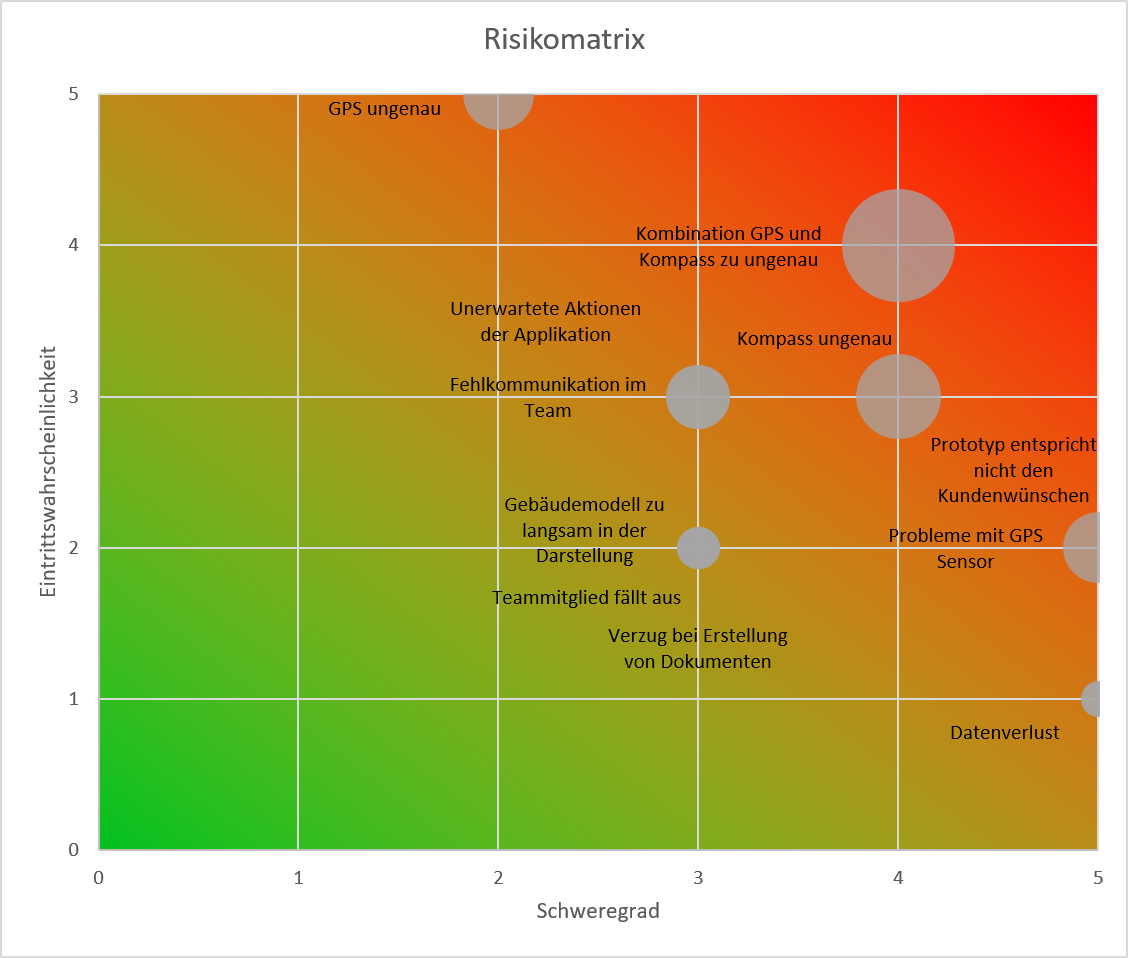
\includegraphics[keepaspectratio, width=0.8\textwidth]{RisikoMatrix}
	\caption{Auswirkungen der Risiken}
\end{figure}

\subsubsection{Massnahmen}

\begin{tabularx}{\textwidth}{|l|X|}
	\hline
	\textbf{Nr.} & \textbf{Beschreibung Massnahme} \\
	\hline
	1 & Alle Wichtigen Daten werden auf externen Diensten ausgelagert, Code und Dokumentation auf GitHub, alle projektrelevanten Dokumente auf OneDrive\\
	\hline
	2 & Sprintmeetings werden in Person durchgeführt, Teammitglieder bemühen sich proaktiv um Kommunikation in Person oder über Messenger und Videochat\\
	\hline
	3 & Alle Arbeiten werden nach CleanCode Praktiken ausgeführt und sauber dokumentiert, sodass das andere Teammitglied übernehmen kann\\
	\hline
	4 & Vorgaben werden periodisch durch Team überprüft, Kontakt mit Betreuer gepflegt\\
	\hline
	5 & Kontakt mit Betreuer wird Proaktiv gesucht und Stossrichtung validiert\\
	\hline
	6 & Nutzer werden Probleme mitgeteilt, Applikation meldet Funktionsbeeinträchtigung\\
	\hline
	7 & Applikation wird nach CleanCode Standards entwickelt und durch Teammitglieder validiert\\
	\hline
	8 & Es werden mehrere Messungen zusammengefasst und der Median deren berechnet\\
	\hline
	9 & In einer Initialisierungsphase wird der Kompass kalibriert\\
	\hline
	10 & Dem Benutzer wird die Möglichkeit gegeben die Initialisierungsphase manuell neu zu starten\\
	\hline
	11 & Das Laden des Gebäudemodells geschieht in der Initialisierungsphase, welche nicht abgeschlossen ist solange das Gebäude nicht verfügbar ist; das Gebäudemodell wird im Detailgrad reduziert, sodass das Laden des Modells schneller vonstatten geht\\
	\hline
\end{tabularx}

\subsubsection{Effekt der Massnahmen}

\vspace{1em}
\noindent
\begin{tabularx}{\textwidth}{|l|X|l|l|l||l|}
	\hline
	\textbf{Nr.} & \textbf{Beschreibung / Risiko} & \textbf{K} & \textbf{S} & \textbf{W} & \textbf{A} \\
	\hline
	1 & Datenverlust & P & 2 & 1 & 2\\
	\hline
	2 & Fehlkommunikation im Team & P & 3 & 1 & 3 \\
	\hline
	3 & Teammitglied fällt aus & P & 3 & 1 & 3 \\
	\hline
	4 & Verzug bei Erstellung von Dokumenten & P & 3 & 1 & 3 \\
	\hline
	5 & Prototyp entspricht nicht den Kundenwünschen & T & 5 & 1 & 5 \\
	\hline
	6 & Probleme mit GPS Sensor & T & 5 & 1 & 5 \\
	\hline
	7 & Unerwartete Aktionen der Applikation & T & 2 & 2 & 4\\
	\hline
	8 & GPS ungenau & T & 2 & 5 & 10\\
	\hline
	9 & Kompass ungenau & T & 4 & 3 & 12\\
	\hline
	10 & Kombination GPS und Kompass zu ungenau & T & 4 & 4 & 16\\
	\hline
	11 & Gebäudemodell zu langsam in der Darstellung & T & 3 & 2 & 6\\
	\hline
\end{tabularx}

\vspace{1em}

\begin{figure}[h!]
	\centering
	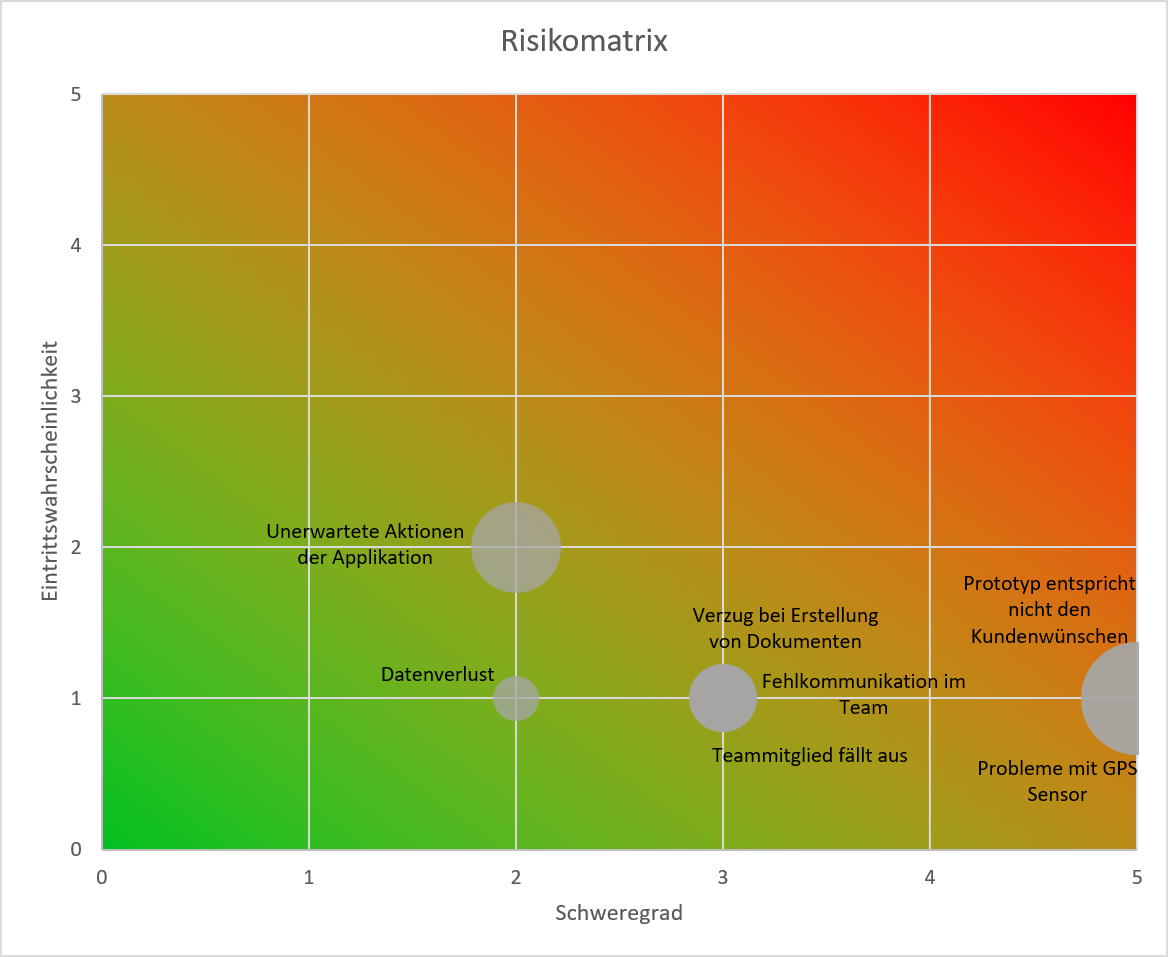
\includegraphics[keepaspectratio, width=0.8\textwidth]{RisikoMatrix_nach_Massnahmen}
	\caption{Risiken nach Massnahmen}
\end{figure}

\chapter{Evaluation und Validation}
\section{Nutzerumfrage}
Um den Stand der Arbeit zu messen und den Erreichungsgrad der Ziele einzuschätzen wurde eine Nutzerumfrage durchgeführt. Diese fand am Freitag 30. November um 11:00 bis 13:00 am Bahnhof Rotkreuz statt. Ziel war es einen möglichst guten Durchschnitt der Bevölkerung und der Demografie der entwickelten Applikation (siehe Tabelle \ref{tab:UserDemografie}) zu erreichen. Im folgenden Kapitel werden der Versuchsaufbau und das Drehbuch erläutert, die Resultate ausgewertet und ein Fazit gezogen.

\begin{table}[htb]
	\centering
	\begin{tabular}{|p{0.2\textwidth}|p{0.2\textwidth}|}
		\hline
		\textbf{Altersgruppe} & \textbf{Prozentsatz} \\
		\hline
		10-20 & 10\% \\
		\hline
		21-30 & 30\% \\
		\hline
		21-45 & 30\% \\
		\hline
		46-65 & 20\% \\
		\hline
		66+ & 10\% \\
		\hline
	\end{tabular}
	\label{tab:UserDemografie}
	\caption{Geschätzte Prozentanteile des Alters an Demografie der Nutzer}
\end{table}

\subsection{Methodik und Drehbuch}
Die Nutzerumfrage wurde folgendermassen durchgeführt: Nach einer kurzen Einleitung über das Projekt wurde dem Probanden die Applikation ohne Erklärung über die Benutzung überreicht. Nachdem sich dieser ein Bild machen konnte, wurden ihm die Fragen des Fragebogens gestellt. Ziel war es den Probanden möglichst nicht zu lange aufzuhalten.

\subsubsection{Drehbuch}

\begin{enumerate}
	\item Begrüssung, Anfragen bezüglich Teilnahme, ansprechen das Toblerone als Dankeschön überreicht wird:
	\textquotedblleft Im Rahmen unseres Industrieprojekt, haben wir eine App entwickelt, welche Neubauten an deren geplanten Position darstellen soll. Dies insbesondere um bei geplanten Projekten neben einer normalen Ausschreibung und den bekannten Stangen, eine visuelle Alternative zu bieten. Diese Befragung dient für uns als Validierung und Sammlung von Verbesserungswünschen.
	Die ganze Befragung dauert in etwa 5Minuten. Und wir würden Ihnen zum Schluss gerne dieses kleine Präsent als Dankeschön für Ihre Hilfe überreichen.\textquotedblright
	\item Übergabe Tablet/Smartphone mit Applikation
	\item Rücknahme Tablet/Smartphone
	\item Fragebogen überreichen / mit Proband durcharbeiten
	\item Danksagung und Verabschiedung
\end{enumerate}

\subsection{Analyse und Resultat}

Insgesamt war die Teilnahmebereitschaft der Probanden auf einem sehr niedrigen Niveau. So erklärten sich von gut 60 Probanden lediglich 13 bereit an der Umfrage teilzunehmen. Die meisten Probanden waren, wie in Abbildung \ref{fig:Altersgruppen} zu sehen, Schüler oder Studenten, welche sich für die Umfrage Zeit nahmen.

\begin{figure}[htb]
	\centering
	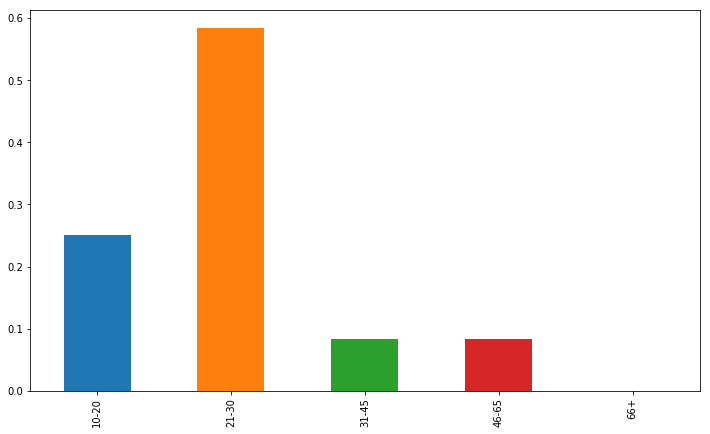
\includegraphics[keepaspectratio, width=0.8\textwidth]{Altersgruppen.png}
	\caption{Anteil der Altersgruppen an der Gesamtheit der Befragung}
	\label{fig:Altersgruppen}
\end{figure}

Die Bewertung der Handhabung wurde insgesamt mit 4.54 (0: unintuitiv, 6: intuitiv) als gut bewertet. Der Grossteil der Probanden wünscht sich eine grössere Präzision bei der Positionierung des Gebäudes. Daneben wurden sich ein Indikator in Richtung des Gebäudes, falls dieses nicht im Blickfeld ist, Hilfetexte und ein Tutorial gewünscht. Von allen Befragten können sich mehr als 90\% vorstellen die Applikation zu gebrauchen, um geplante Neubauten anzusehen (siehe Abbildung \ref{fig:Nutzung}).

\begin{figure}[htb]
	\centering
	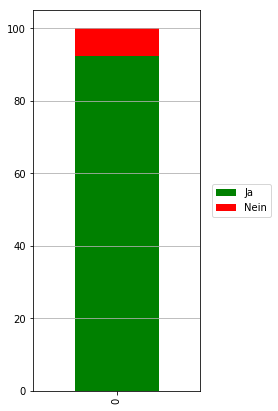
\includegraphics[keepaspectratio, width=0.3\textwidth]{Nutzung.png}
	\caption{Prozentanteile für die Nutzung der Applikation}
	\label{fig:Nutzung}
\end{figure}

Als zusätzliche Nutzungsmöglichkeiten wurden neben der Betrachtung einer Immobilie (Apartments, Neubau, geplantes Gebäude) von aussen, auch die Visualisierung von Gebäuden für den Unterricht (beispielsweise Geschichtsunterricht oder gestalterisches Zeichnen) und eine Art Röntgenblick für Gebäude genannt.

\subsection{Fazit}
Die gewünschte Zieldemografie konnte durch geringe Teilnahme nicht erreicht werden. Es besteht jedoch auf jeden Fall Marktpotenzial für die Applikation; mehr als 90\% der Probanden gaben an die Applikation zu nutzen, falls Sie verfügbar würde. Die Bedienbarkeit der Applikation wurde als intuitiv und gut bewertet, es wurden jedoch ein Tutorial, Hilfetexte am Gebäude und Indikatoren zur Verbesserung gewünscht. Es wurden auch interessante Alternativnutzungen vorgeschlagen, wie beispielsweise als Hilfsmittel in der Bildung und für einen detaillierten Einblick über die Innenstruktur von ausserhalb.

\section{Vergleich mit Anforderungen}
\label{sec:VergleichAnforderungen}
Hier werden die Anforderungen aufgelistet und ob diese erfüllt wurden oder nicht. Sofern diese nicht erfüllt wurden, wird für deren Erfüllung eine potenzielle Lösungsidee beschrieben. Für die Verifikation wurden die Testfälle überprüft.
\bigbreak
Legende:
<<\checkmark >> = Anforderung erfüllt, <<x>> = Anforderung nicht erfüllt, <<->> Wurde aus Zeitgründen nicht Implementiert.

\begin{tabularx}{\textwidth}{l l X}
\hline
	\# & \textbf{Erfüllt?} & \textbf{Beschreibung} \\
\hline
	1.1 & x & Das Augmented Reality Objekt soll ausserhalb von Gebäuden eine maximale Abweichung von 10m auf einer minimalen Distanz von 50m bis zu einer Distanz von 1km auf korrekter Position dargestellt werden \\
\hline
	1.2 & \checkmark & Das Augmented Reality Objekt soll ausserhalb von Gebäuden eine maximale Rotationsabweichung von \ang{10} aufweisen.\\
\hline
	1.3 & \checkmark & Das Augmented Reality Objekt soll ausserhalb von Gebäuden eine maximale Grössenunterschied von 5\% zum Original Aufweisen.\\
\hline
	1.4 & \checkmark & Das Augmented Reality Objekt soll ausserhalb von Gebäuden mit einer Maximalen Verzögerung (bei Bewegung) von <1 Sekunde reagieren.\\
\hline
	1.5 & \checkmark & Das Augmented Reality Objekt soll ausserhalb von Gebäuden nach Beendigung von langsamen(<=10km/s) Bewegungen der Kamera auf der korrekten Position bleiben.\\
\hline
	1.6 & \checkmark & Das Augmented Reality Objekt soll ausserhalb von Gebäuden nach Beendigung von mittelmässig schnellen (>10km/s und <=20km/s) Bewegungen wieder auf korrekter Position dargestellt werden.\\
\hline
	1.7 & \checkmark & Das Augmented Reality Objekt soll ausserhalb von Gebäuden nach Beendigungen von schnellen (>20km/s) Bewegungen nach einer erneuten Initialisierung wieder auf korrekter Position dargestellt werden.\\
\hline
	1.8 & \checkmark & Das Augmented Reality Objekt soll ausserhalb von Gebäuden nur in einer Distanz bis mindestens 1km dargestellt werden (gilt auch für alle Informationen zum Objekt).\\
\hline
	2 & - & Sobald das Objekt ausserhalb des Sichtfeldes ist, soll dem Benutzer eine Anzeige für das Wiederauffinden des Objektes angezeigt werden.\\
\hline
	3 & - & Sofern keine Informationen zur Lokalisierung vorhanden sind soll der Benutzer in weniger als 3 Sekunden über diese fehlende Informationen informiert werden. \\
\hline
\end{tabularx}

\subsection{Verbesserung für \#1.1}
Um die Anforderung von 1.1 erfüllen zu können, müsste die Nordinitialisierung erheblich verbessert werden, da dieser den ungenauesten Sensor darstellt. Eine potenzielle Lösung für dieses Problem kann die kontinuierliche Berechnung von Norden mit den Bewegungen des Smartphones darstellen. Dies ist jedoch in der zur Verfügung stehenden Zeit nicht Lösbar gewesen.

\subsection{Verbesserung für \#2}
Um die Anforderung von Nummer 2 erfüllen zu können, wird ein Indikator, welcher die Richtung des ausser Sichtweite geratenen Objekt anzeigt, benötigt. Kudan liefert bereits die Möglichkeit die Position zum Viewpoint zu berechnen. Damit lässt sich die Position des Pfeiles bestimmen und er kann an der korrekten Position dargestellt werden. Die Implementierung konnte jedoch aus zeitlichen Gründen nicht durchgeführt werden.

\subsection{Verbesserung für \#3}
Die momentane Architektur lässt es mit einfachen Anpassungen zu, dass die Activity selbst über Location Updates informiert wird. So müsste, um diese Anforderung zu erfüllen die Activity das Interface LocationFilterListener implementieren und sich selber bei LocationFilter registrieren. So würde die Activity über alle LocationUpdates informiert werden. Um nun dem Benutzer die Information anzuzeigen, müsste im Hintergrund ein Timer laufen, welcher nach 3 Sekunden eine Information an den Benutzer liefert. Bei eingegangene Location müsste der Timer wieder zurückgesetzt werden. Die Implementierung konnte jedoch aus zeitlichen Gründen nicht durchgeführt werden.

\section{Projekt Fazit}
Die Projektarbeit im Rahmen dieses Moduls hat uns sehr viel gelehrt. Wir konnten wertvolle Erkenntnisse sammeln und können nun besser einschätzen, was uns bei der Bachelorarbeit erwartet. Die Zusammenarbeit und Kommunikation innerhalb des Teams verlief einwandfrei, auch die Kommunikation mit dem Betreuer war sehr gut und angenehm.

Im nachfolgenden Abschnitt schildern wir was wir gelernt haben und was wir bei unserem nächsten Projekt besser lösen werden.
Der erste Punkt, welchen wir verbessern werden, ist mit der Dokumentation früher im Projekt zu beginnen.  Die Dokumentation ist nicht erst während der letzten Wochen entstanden, aber es gab viele Punkte, die bis zum Schluss nicht ganz klar und somit noch nicht dokumentiert waren.

Ein weiterer Punkt zur Verbesserung wäre, dass wir uns schneller auf eine Plattform und ein Framework beschränken. Eine Eingrenzung der Plattform und des Frameworks hätte früher im Projekt eine Abgrenzung gesetzt und die Entwicklung des eigentlichen Prototyps fokussiert und somit beschleunigt.

Weiter haben wir den Aufwand für die Literaturrecherche und das Schreiben der Stand der Forschung massiv unterschätzt, wir werden diese Aktivität beim nächsten Projekt früher angehen und höher priorisieren.

Weiter können wir auch in diesem Projekt entstandene Artefakte weiter nutzen. So konnten wir den Umgang mit den Hilfsmitteln stärker vertiefen. Zudem konnte für die Dokumentation sowie den Code der Git Feature Branch Workflow etabliert werden, welche das simultane Arbeiten stark vereinfachte und einen optimalen Code und Dokumentationsüberprüfung des anderen Projektmitgliedes forcierte. Ein weiterer Vorteil ist zudem das nun vorhandene Wissen wie eine CI \& CD Infrastruktur für Code sowie Dokumentation früher und effizienter aufgebaut werden können.

Wie im Unterkapitel \ref{sec:VergleichAnforderungen} beschrieben wurde nur ein Subset der Anforderungen erfüllt. Dennoch konnte in der Nutzerumfrage bewiesen werden, dass die Nutzer ein Interesse an der Applikation besitzen und einen reellen Nutzen sehen. Es konnten jedoch wichtige Funktionalitäten nicht realisiert werden, welche für eine Markteinführung noch implementiert werden müssten. Diese schildern wir im Ausblick (siehe \ref{sec:Ausblick}) im Detail.

\section{Ausblick}
\label{sec:Ausblick}
Um die im Rahmen dieser Arbeit entwickelte und realisierte AR Applikation in ein marktreifes Produkt zu verwandeln, wäre es noch nötig den bestehenden Code um folgende Aspekte zu verbessern:

\begin{itemize}
	\item Implementation von Anforderungen 2 und 3
	\item Implementierung von Unittests
	\item Erstellen einer CD Pipeline
	\item Verbesserung der Initialisierung gegen Norden
	\item Verbesserung der Höhenlogik mit OpenElevation
	\item Implementation einer GPS Lösung mit SLAM Implementierung (damit könnte die Darstellungsgenauigkeit verbessert werden)
	\item Verbesserung des GUI
	\item Implementation der Serverseite mit dazugehörender Client Logik
	\item Implementation einer Schnittstelle um neue Gebäude auf Server hochzuladen
	\item Implementation einer iOS Lösung
\end{itemize}

\appendix

\glossary{Abkürzungsverzeichnis}

\listoffigures

\listoftables

\listofmyequations \pagebreak

\printbibliography

\chapter{Testprotokolle}
\label{appendig:testprotokolle}
\section{Testprotokoll 28.11.2018}
Dieses Protokoll wurde von Dane Wicki am 28.11.2018 erstellt.
\subsection{T-001v1}
Test liefert erwartetes Ergebnis.
\subsection{T-002v1}
Test liefert erwartetes Ergebnis.
\subsection{T-003v2}
Test liefert erwartetes Ergebnis.
\subsection{T-004-v2}
Test liefert erwartetes Ergebnis.
\subsection{T-005-v2}
Test liefert erwartetes Ergebnis.
\subsection{T-006-v2}
Test liefert erwartetes Ergebnis.
\subsection{T-007-v2}
Test liefert erwartetes Ergebnis.
\subsection{T-008-v1}
Test liefert erwartetes Ergebnis.
\subsection{T-009-v2}
Test liefert erwartetes Ergebnis.
\subsection{T-010 und Folgende}
Wurden nicht durchgeführt
\section{Testprotokoll 04.12.2018}
Dieses Protokoll wurde von Dane Wicki am 04.12.2018 erstellt.
\subsection{T-001v1}
Test liefert erwartetes Ergebnis.
\subsection{T-002v1}
Test liefert erwartetes Ergebnis.
\subsection{T-003v2}
Test liefert erwartetes Ergebnis.
\subsection{T-004-v2}
Test liefert erwartetes Ergebnis.
\subsection{T-005-v2}
Test liefert erwartetes Ergebnis.
\subsection{T-006-v2}
Test liefert erwartetes Ergebnis.
\subsection{T-007-v2}
Test liefert erwartetes Ergebnis.
\subsection{T-008-v1}
Test liefert erwartetes Ergebnis.
\subsection{T-009-v2}
Test liefert erwartetes Ergebnis.
\subsection{T-010-v1}
Test wurde nicht erfüllt.
Das Darstellung des Gebäudes weist teilweise stärkere Abweichungen als erlaubt auf. Diese Abweichungen hängen stark von der korrekten Nordausrichtung des Smartphones zusammen.
Mit einem Abstand zum Gebäude von ca. 80m wurden insgesammt 10 Testdurchfürungen durchgeführt. Die Höhenungenauigkeit wurde bei diesen durchführungen lediglich das augenmas verewendet. Für die X und Y abweichungen wurde das Smartphone auf bedennähe gebracht und dort Fixiert, damit die Position des Smartphones glechbleibt. Anschliessend wurde auf sichtlinie in ca. 50cm abstand ein Marker für den Rand des Physikalischen gebäudes auf den Boden des Sichtbereiches gelegt. Danach wurde für denselben Rand des Virtuellen Gebäudes ein weiterer Marker in der Gleichen Distanz auf den Boden gelegt. Danach konnte mittels Trigonometrie die ungefähre Abweichung berechnet werden (siehe Abbildung \ref{fig:TrigometrieBeispiel})


\begin{figure}[h!]
	\center
	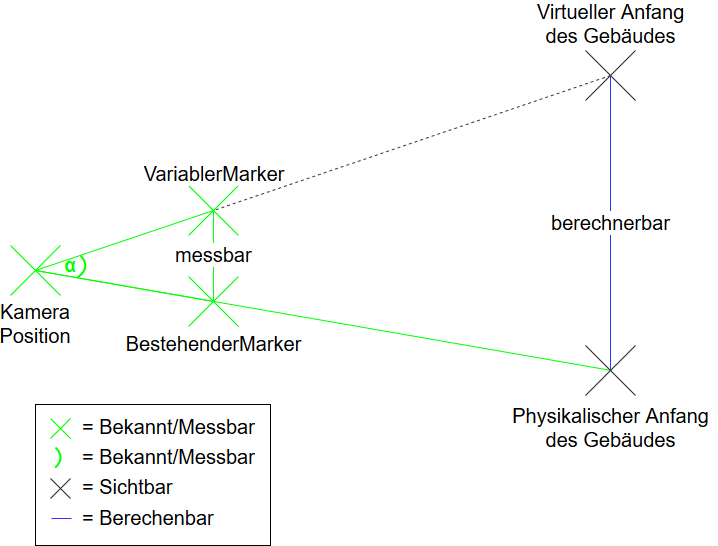
\includegraphics[keepaspectratio, width=\textwidth / 2]{TrigonometrieBeispiel.png}
	\caption{Beispiel der Verwendeten Trigonometrie}
	\label{fig:TrigometrieBeispiel}
\end{figure}

Die 10 Messungen ergaben folgende Abweichungen (gerundete auf einen Meter):
\begin{enumerate}
	\item 8m
	\item 15m
	\item 4m
	\item 7m
	\item 2m
	\item 19m
	\item 5m
	\item 14m
	\item 9m
	\item 12m
\end{enumerate}
\subsection{T-011-v1}
Durch die Bedingungen dieses Test, wurde bei jeder Korrekten Position (<10m Abweichung) von Augenmass die Abweichung des Gebäudes überprüft. Es konnten keine Grössenunterschiede festgestellt werden.
\subsection{T-012-v1}
Durch die Bedingungen dieses Test, wurde bei jeder Korrekten Position (<10m Abweichung) von Augenmass die Abweichung des Gebäudes überprüft. Es konnten keine Rotationsabweichungen festgestellt werden.
\subsection{T-013-v1}
Durch die Bedingungen dieses Test, wurde bei jeder Korrekten Position (<10m Abweichung) von Augenmass die Abweichung des Gebäudes überprüft nach durchführung des Testes.
Dieser Test wurde 3 mal durchgeführt, für jede Stärke (siehe \ref{ch:Anforderungen}) der Erschütterung.
Alle 3 Test haben bestanden.
\subsection{T-014-v1}
Durch die Bedingungen dieses Test, wurde bei jeder Korrekten Position (<10m Abweichung) von Augenmass die Darstellungsgeschwindigkeit des Gebäudes überprüft. Es konnten keine starken (> eine Sekunde) Verzögerungen festgestellt werden.
\subsection{T-015-v1}
Test liefert erwartetes Ergebnis.
\chapter{Sprints}

\begin{figure}[h!]
	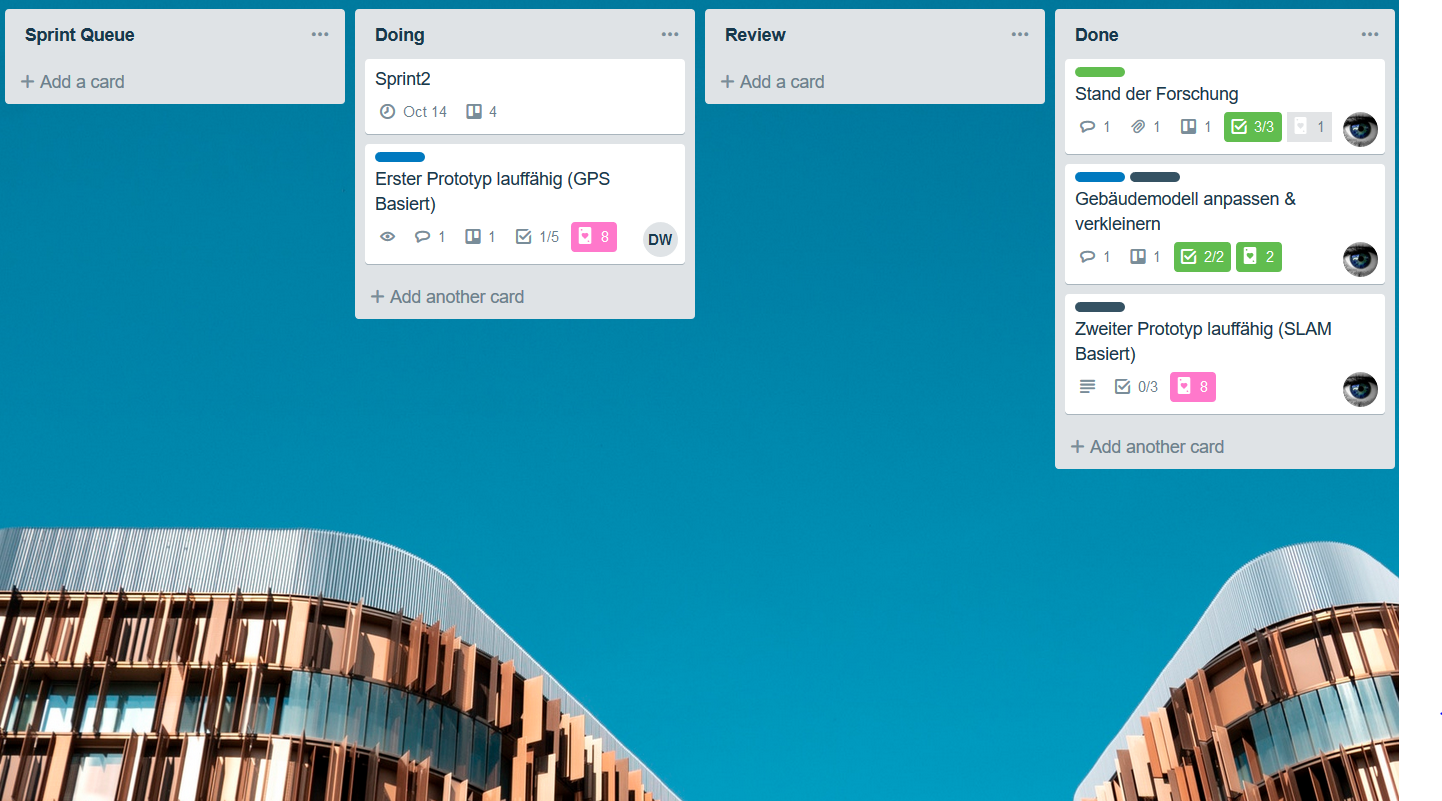
\includegraphics[keepaspectratio,width=\textwidth]{SprintReview_2}
	\caption{Erledigte Tasks in Sprint 2}
\end{figure}

\begin{figure}[h!]
	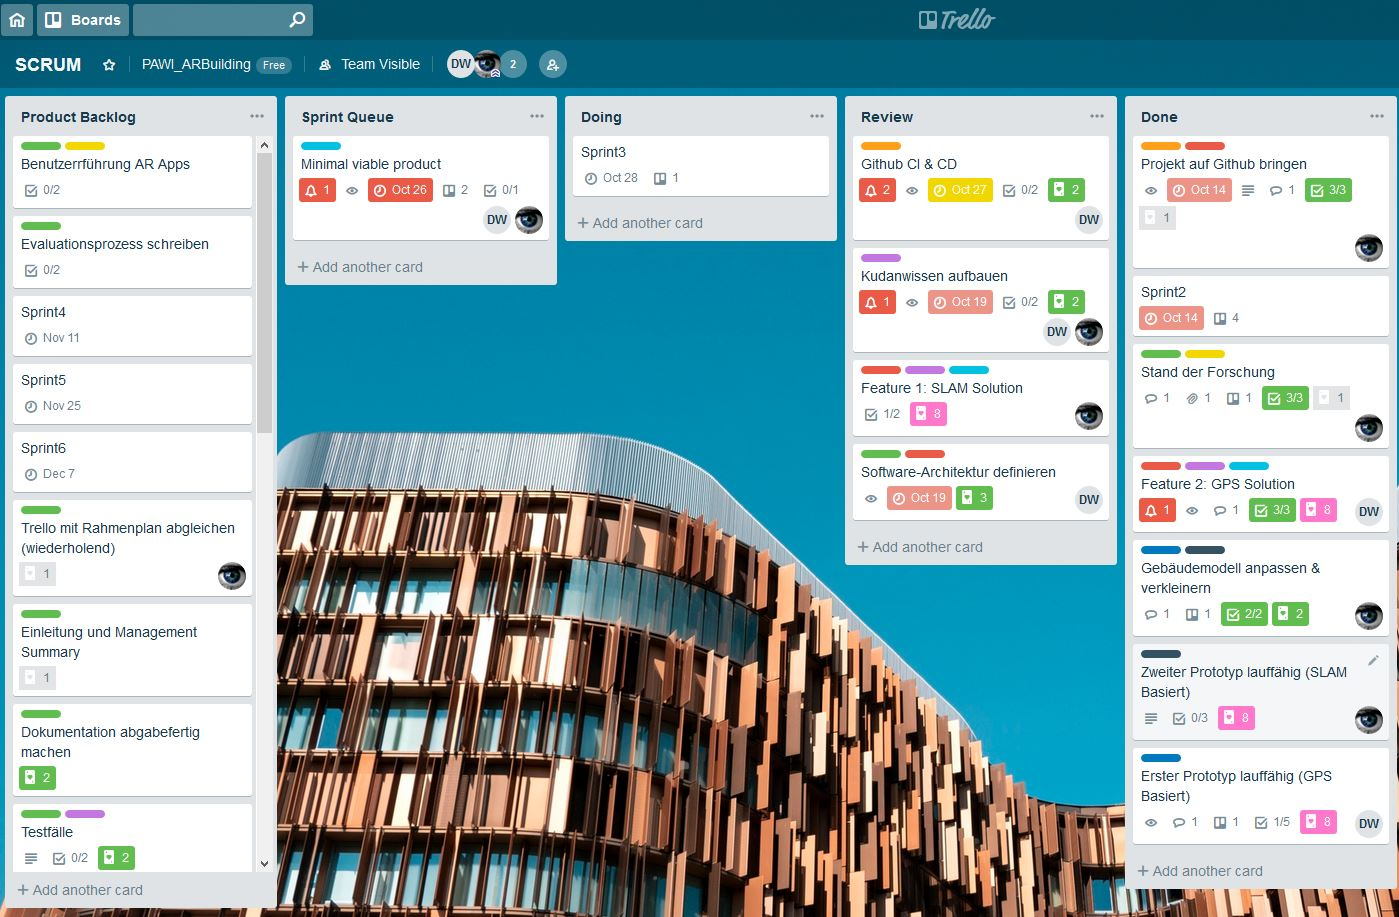
\includegraphics[keepaspectratio,width=\textwidth]{SprintReview_3}
	\caption{Erledigte Tasks in Sprint 3}
\end{figure}

\newpage

\begin{figure}[h!]
	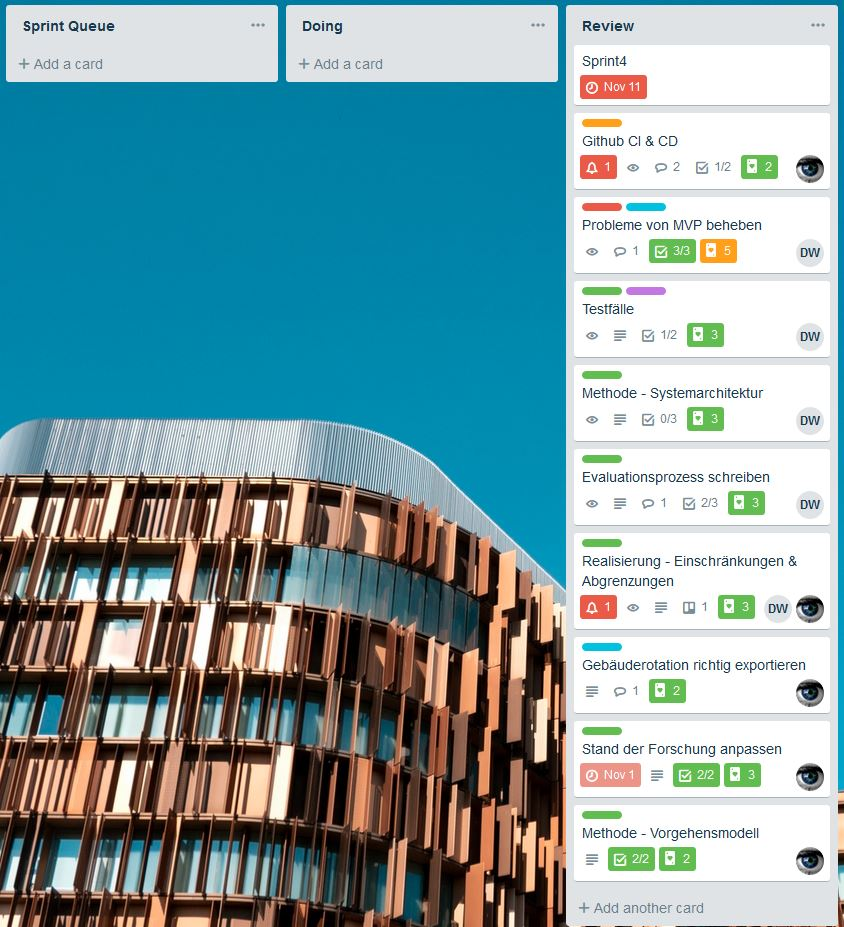
\includegraphics[keepaspectratio,width=\textwidth]{SprintReview_4}
	\caption{Erledigte Tasks in Sprint 4}
\end{figure}

\newpage

\begin{figure}[h!]
	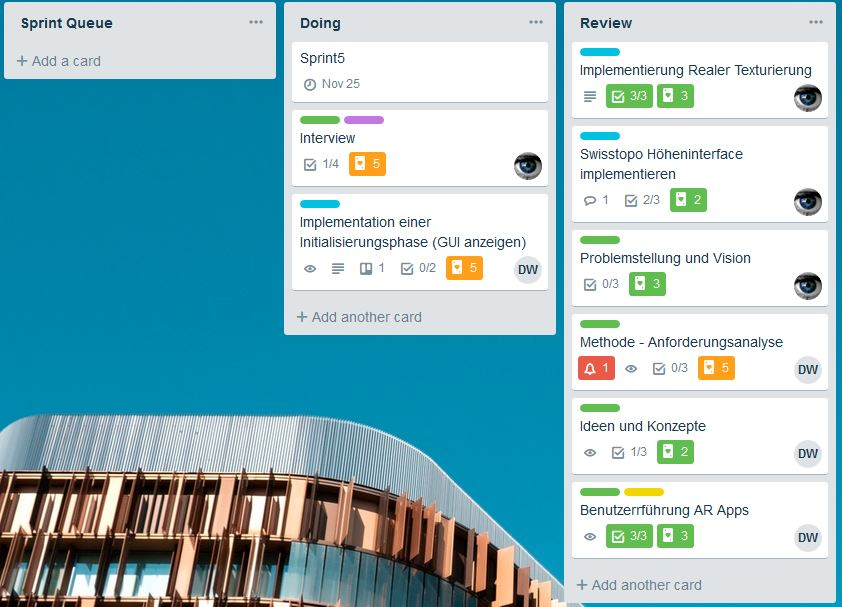
\includegraphics[keepaspectratio,width=\textwidth]{SprintReview_5}
	\caption{Erledigte Tasks in Sprint 5}
\end{figure}

\newpage

\chapter{Evaluationen}

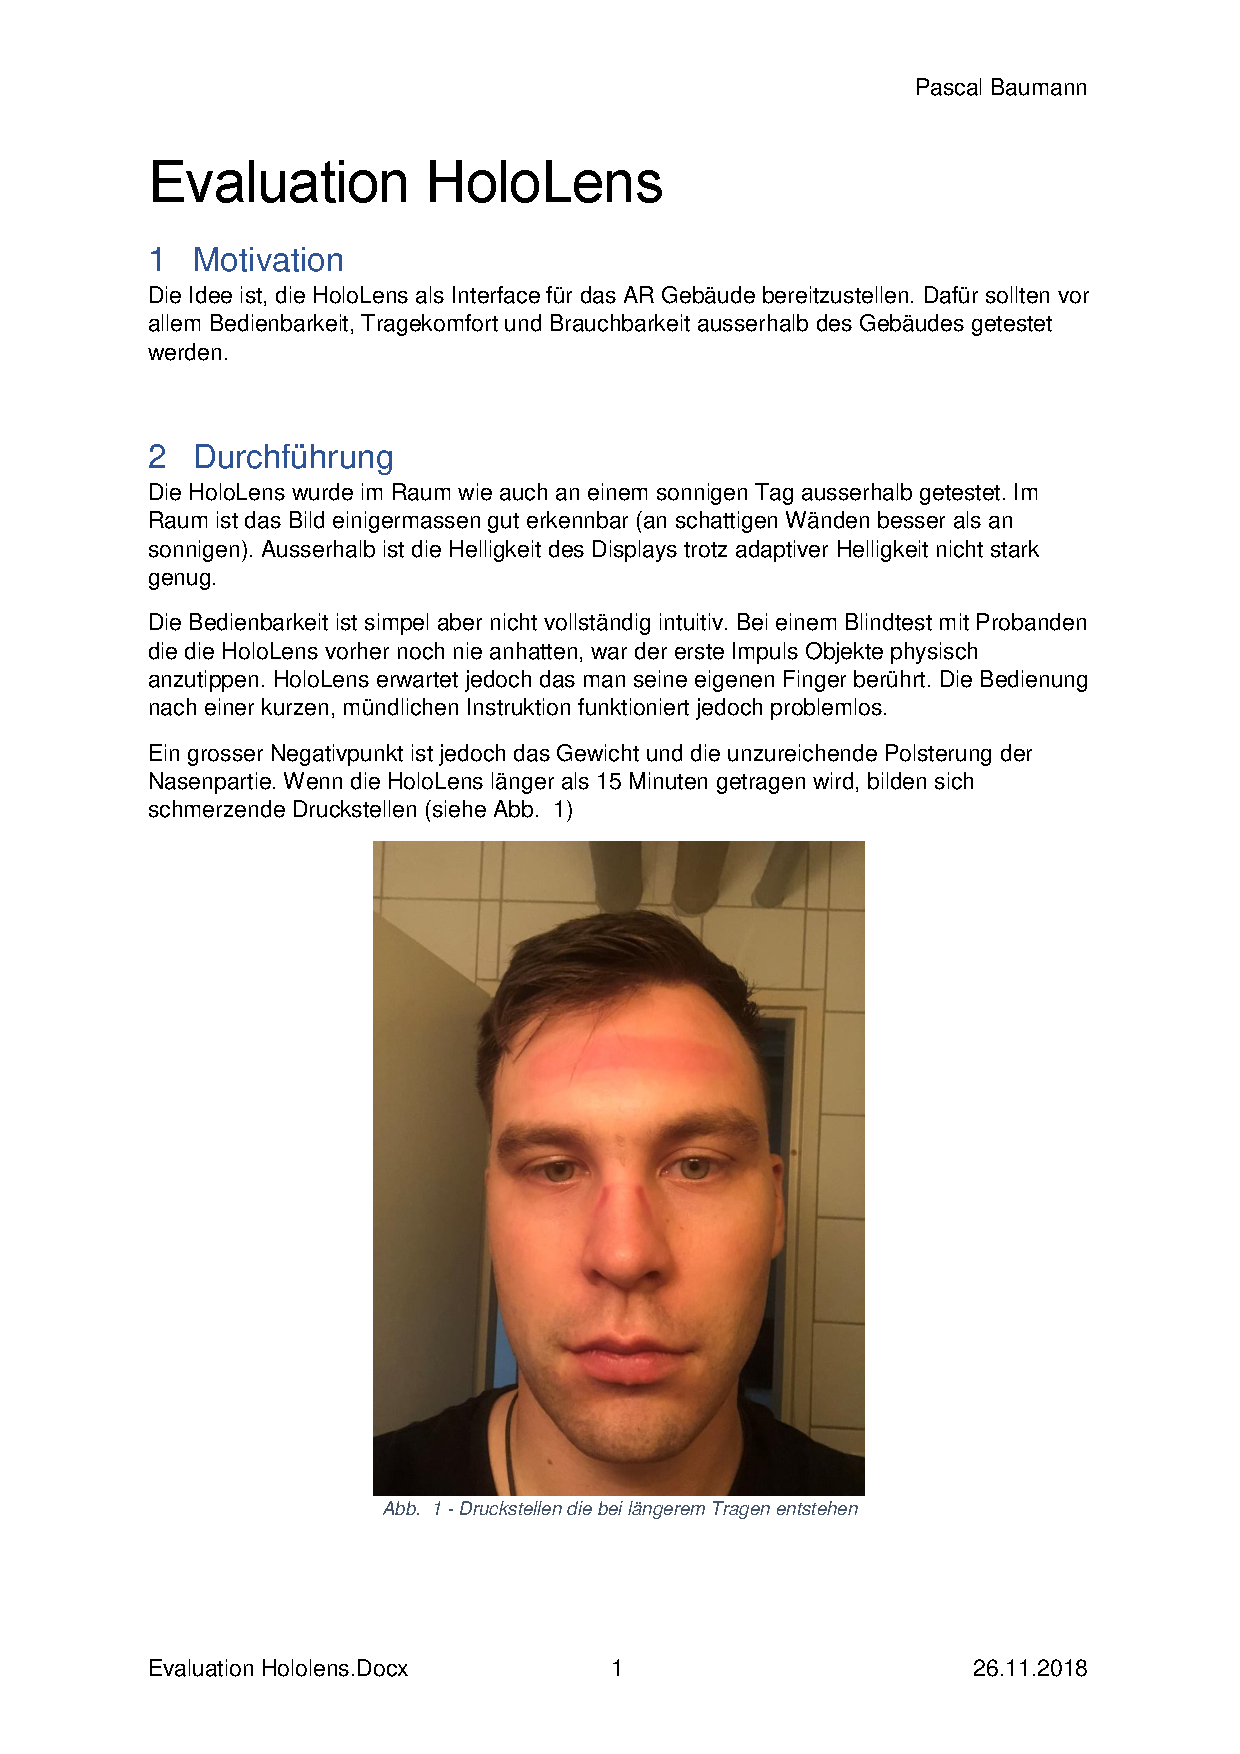
\includepdf[pages=-]{Evaluation_HoloLens.pdf}

\chapter{Anleitungen}

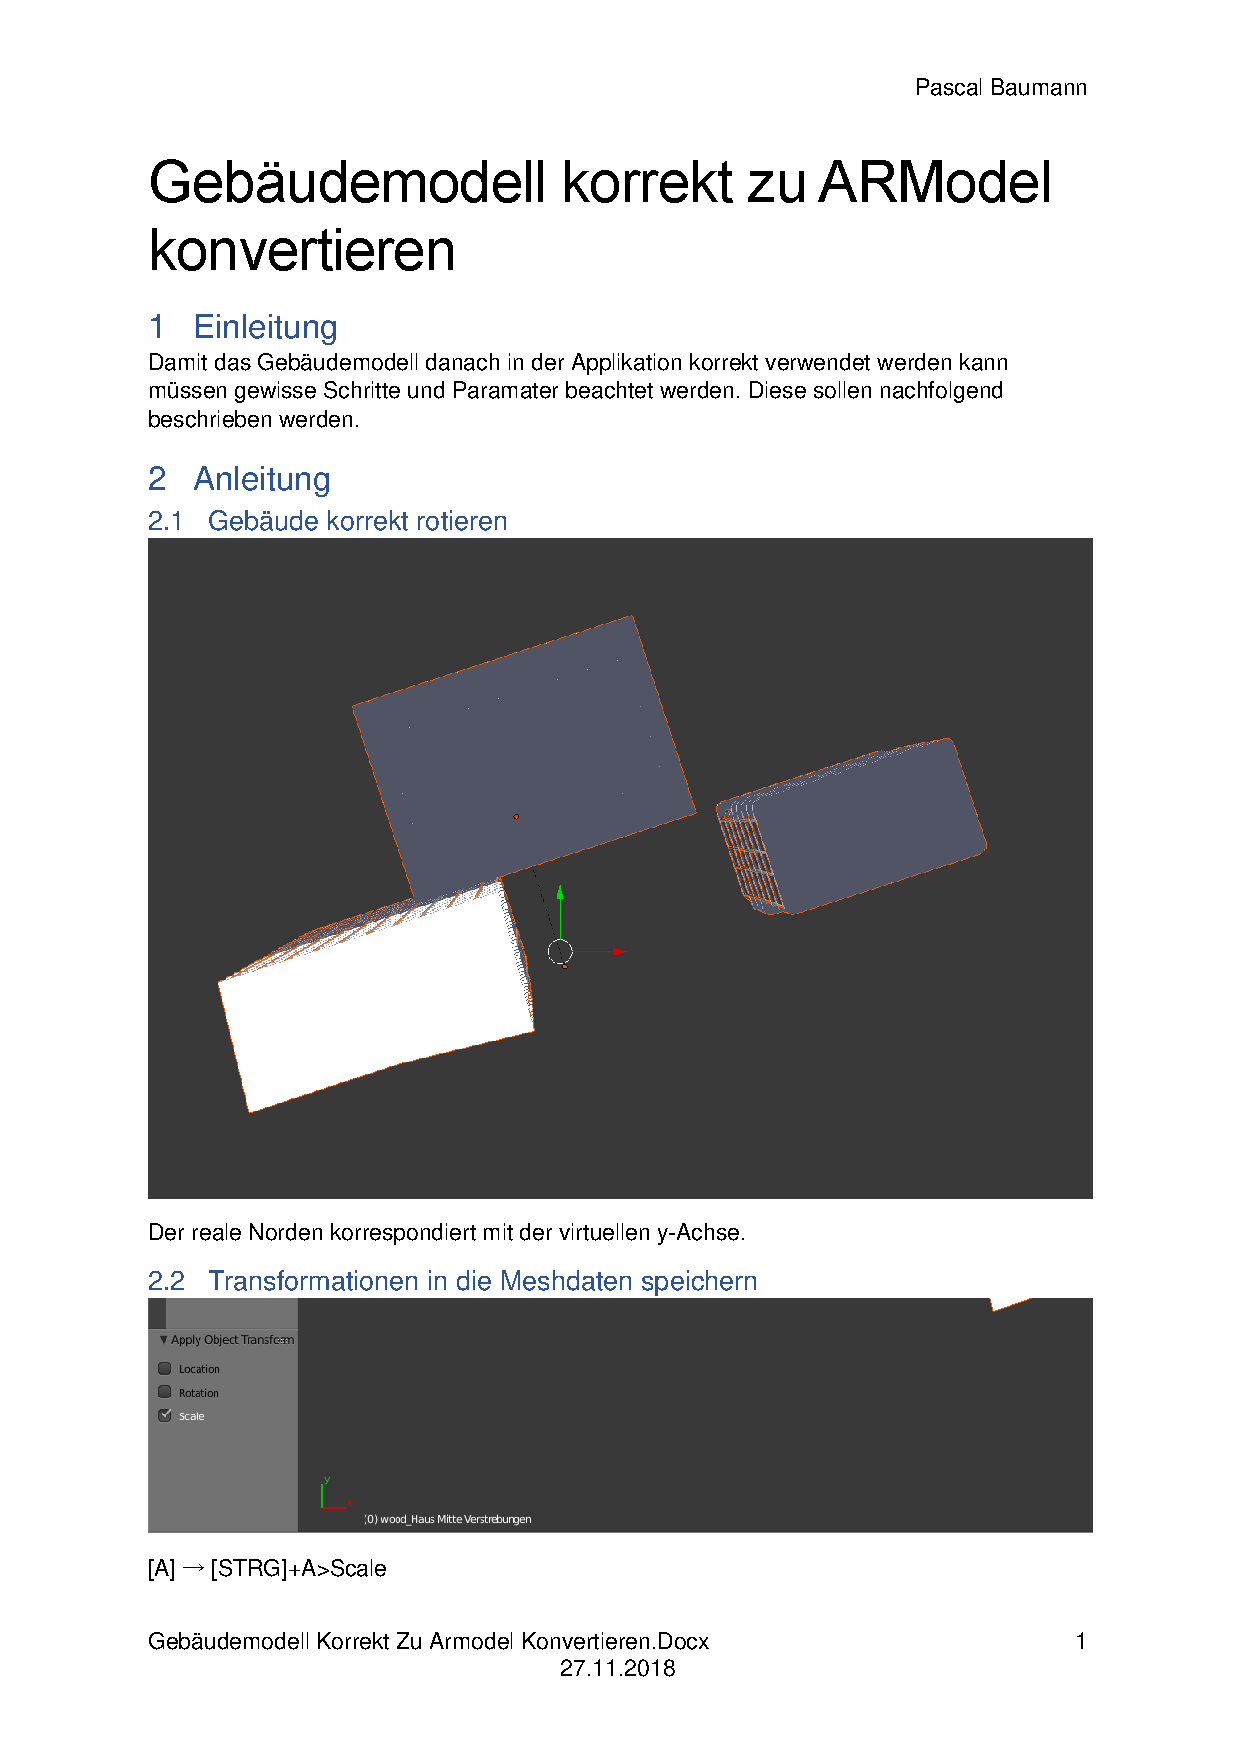
\includepdf[pages=-]{Gebaeudemodell_korrekt_zu_ARModel_konvertieren.pdf}

\chapter{Daten der Nutzerbefragung}

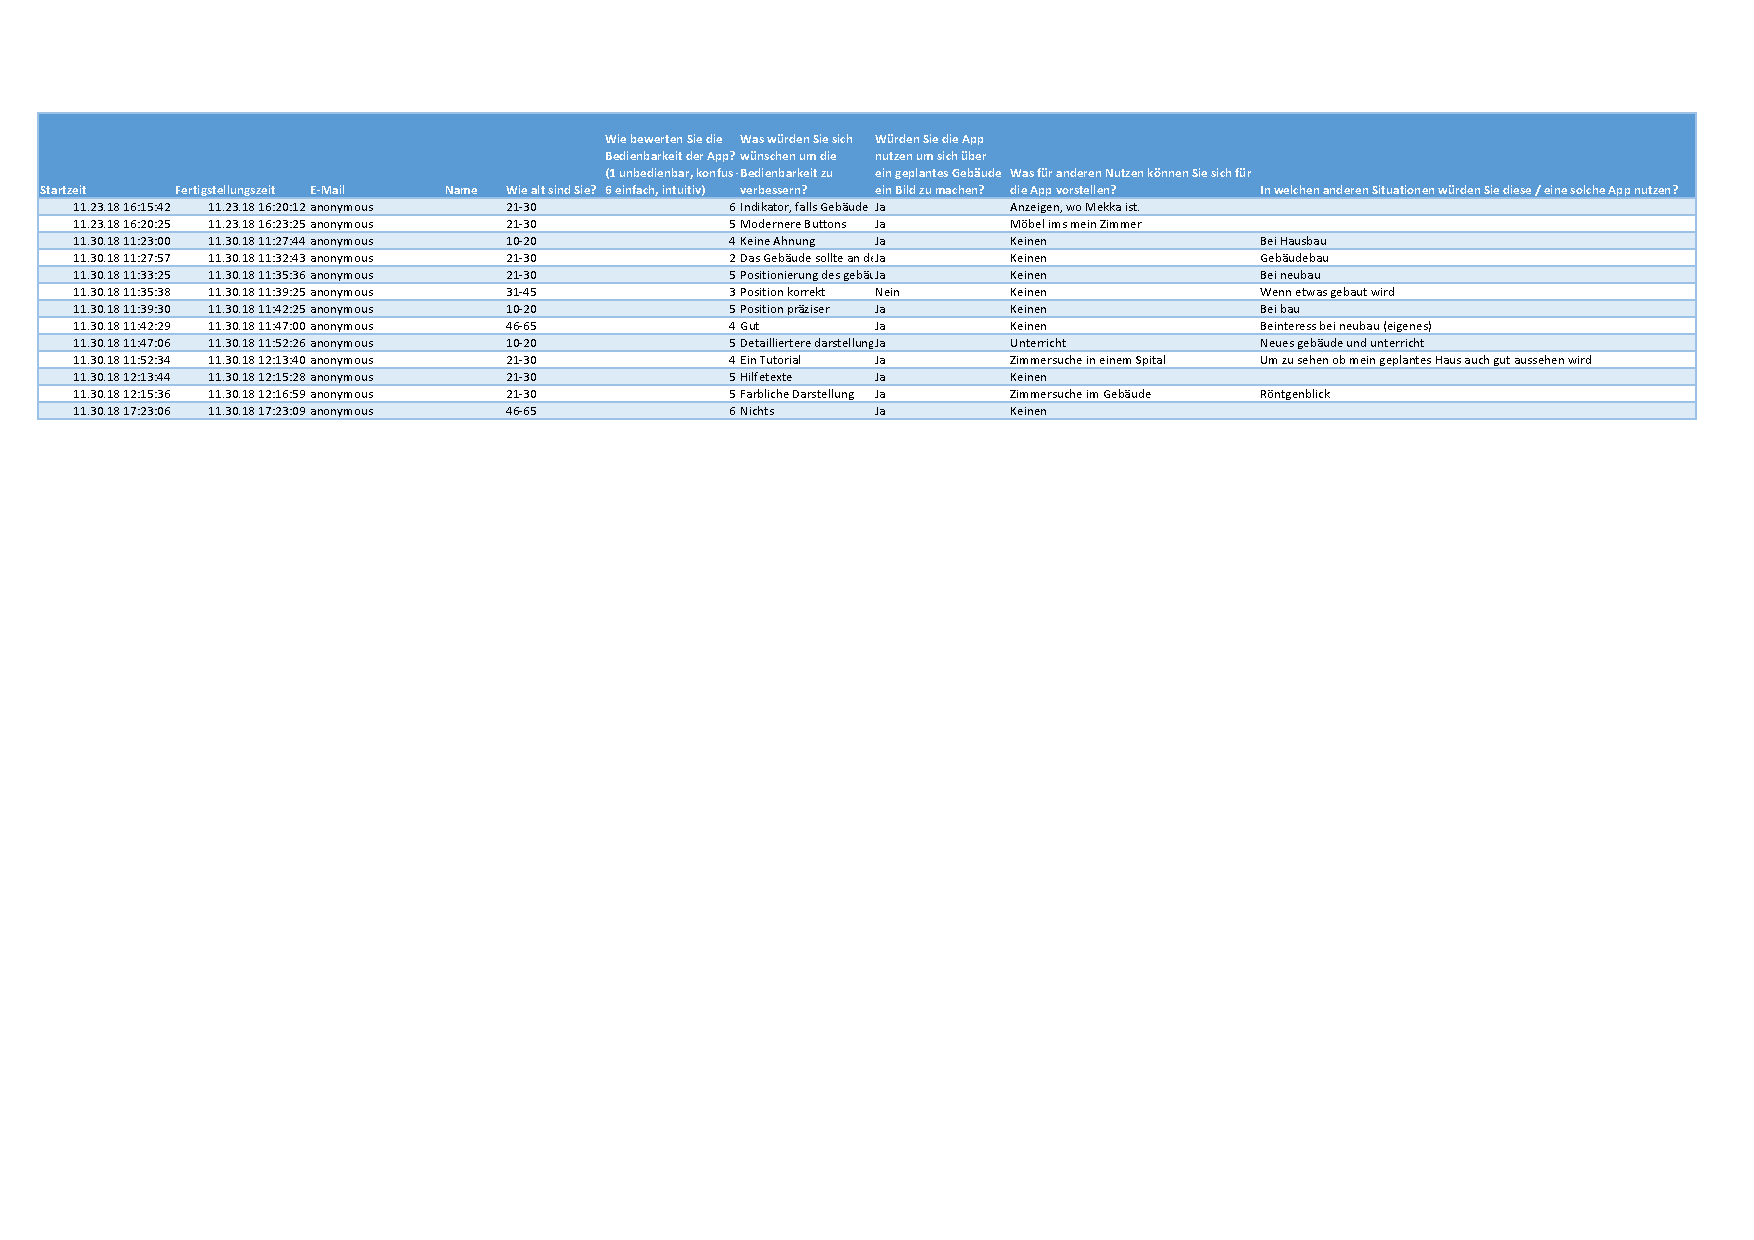
\includepdf[pages=-]{Nutzerbefragung_Rohdaten.pdf}

\chapter*{Eidesstattliche Erklärung}
Ich erkläre hiermit, dass ich/wir die vorliegende Arbeit selbständig und ohne unerlaubte fremde Hilfe angefertigt haben, alle verwendeten Quellen, Literatur und andere Hilfsmittel angegeben haben, wörtlich oder inhaltlich entnommene Stellen als solche kenntlich gemacht haben, das Vertraulichkeitsinteresse des Auftraggebers wahren und die Urheberrechtsbestimmungen der Fachhochschule Zentralschweiz (siehe Merkblatt «Studentische Arbeiten» auf MyCampus) respektieren werden.

\vspace{1em}

\renewcommand{\arraystretch}{2}
\begin{tabularx}{\textwidth}{XXXX}
	Unterschrift: & & Unterschrift: & \\ \cline{2-2}\cline{4-4}
	Baumann, Pascal & & Wicki, Dane & \\
	Datum: & & Ort: & \\
\end{tabularx}

\end{document}
